\documentclass{article}


\usepackage{arxiv}

\usepackage[utf8]{inputenc} % allow utf-7 input
\usepackage[T1]{fontenc}    % use 8-bit T1 fonts
\usepackage{hyperref}       % hyperlinks
\usepackage{url}            % simple URL typesetting
\usepackage{booktabs}       % professional-quality tables
\usepackage{amsfonts}       % blackboard math symbols
\usepackage{nicefrac}       % compact symbols for 1/2, etc.
\usepackage{microtype}      % microtypography
\usepackage{lipsum}
\usepackage{graphicx}
\graphicspath{ {./images/} }

\usepackage{lmodern}%
\usepackage{textcomp}%
\usepackage{lastpage}%
% \usepackage[margin=0.5in]{geometry}%
\usepackage{float}%
\usepackage{xcolor}
\usepackage[export]{adjustbox}
\usepackage[numbers]{natbib}
\usepackage{listings}
\usepackage{minted}
\usemintedstyle{vs}
\usepackage{subfig}
\usepackage{multirow}

\renewcommand{\arraystretch}{1.5}



\title{A Comprehensive Neural Network Potential for Al-Cu}

\author{
 Daniel Marchand \\
  Institute of Materials Science \\
  École Polytechnique Fédérale de Lausanne \\
  CH-1015, Vaud, Switzerland \\
  \texttt{daniel.marchand@epfl.ch} \\
  %% examples of more authors
   \And
 Albert Glensk \\
  Institute of Mechanical Engineering \\
  École Polytechnique Fédérale de Lausanne \\
  CH-1015, Vaud, Switzerland \\
  \texttt{albert.glensk@epfl.ch} \\
  \And
 William Curtin \\
  Institute of Mechanical Engineering \\
  École Polytechnique Fédérale de Lausanne \\
  CH-1015, Vaud, Switzerland \\
  \texttt{william.curtin@epfl.ch} \\
  %% \AND
  %% Coauthor \\
  %% Affiliation \\
  %% Address \\
  %% \texttt{email} \\
  %% \And
  %% Coauthor \\
  %% Affiliation \\
  %% Address \\
  %% \texttt{email} \\
  %% \And
  %% Coauthor \\
  %% Affiliation \\
  %% Address \\
  %% \texttt{email} \\
}

\begin{document}
\maketitle
\begin{abstract}
Precipitates are fundamental to the strengthening of aluminum alloys, and understanding them is paramount for optimized processing.
Precipitates are highly complex, and their formation sequence, kinetics, and the resulting influence on mechanical properties must be studied at the atomic scale, particularly during early-stage nucleation and growth.
Atomistic modeling via Density Functional Theory (DFT) is well-established and has been successful for a wide variety of precipitates; however, it is extremely computationally expensive and typically limited to modeling relatively simple bulk properties. On the contrary, interatomic potentials are computationally affordable, yet tend to lack accuracy. A promising new method for modeling precipitates is through the use of interatomic Neural Network Potentials (NNPs), that have near-DFT accuracy without the massive cost. 
Here, we present a demonstration of NNPs for Al-Cu based-alloys, 
their $\theta''$ $\rightarrow$ $\theta'$ $\rightarrow$ $\theta$ precipitation sequence
being one of the oldest and most investigated in the field, providing a model system for comparison.
We demonstrate the high fidelity of the Al-Cu NNPs for predictions of intermetallic compound energetics, elasticity, dilute solid-solution binding, interfaces, generalized stacking fault energy surfaces, and antisite defect energies.
We further show that our NNP can correctly capture the subtle, entropically-induced shift between $\theta'$ and $\theta$.
This work points to a new and powerful approach for advancing the predictive understanding of Al alloys. 
\end{abstract}


% keywords can be removed
%\keywords{First keyword \and Second keyword \and More}

\section{Introduction}
The mechanical properties of metals that make them widely useful for many structural applications are related to the underlying fundamental behavior of defects in the crystalline lattice.  The atomic structures of dislocations, grain boundaries, interfaces, precipitates, crack tips, and vacancies and their motion, evolution, and/or interactions all determine the plastic flow, fracture toughness, creep, fatigue, radiation resistance, and other essential macroscopic performance measures.  Most engineering metals are alloys, i.e., multicomponent and multiphase materials, adding another level of chemical complexity beyond that of the defects themselves.  Understanding, and ultimately controlling, the behavior of these defects is crucial for optimizing application conditions and designing new higher-performance alloys.  This, in turn, requires atomic-scale simulations but at scales relevant to the defects that are often far above the scales accessible by first-principles methods such as density-functional theory (DFT).  The solution is thus the development of semi-empirical interatomic potentials that accurately capture the structures, energies, and motion of the various defects.

The development of interatomic potentials has a long history.
Some are special-purpose, aimed at capturing one or a few specific properties of relevance for a narrow range of behavior.
Other potentials are intended to be for broader use across different defects in a given metal.
Potentials for elemental FCC metals, mainly within the embedded-atom or modified embedded-atom (EAM and MEAM, respectively) frameworks, are widespread, and generally perform well against experimental or first-principles benchmarks to which they are fit while providing adequate representations of many defects.
However, even potentials for FCC metals can be very inaccurate for certain properties, e.g., unstable stacking fault energies, or can predict unphysical behavior for a given defect, e.g., a sharp crack tip.
Potentials for FCC alloys generally have even more limited capabilities, due to the underlying assumptions of the embedded atom framework, such that the potentials are only reasonably quantitative for a few properties.
Potentials for BCC elements and alloys are far less successful, with almost no potentials able to produce the proper correct compact and unpolarized screw dislocation core and Peierls potential for screw motion, which controls plasticity in elemental BCC metals.
Potentials for elemental HCP metals are also less successful because the range of operative slip systems (basal, prismatic, pyramidal I, and II) is broad and high-temperature transitions to BCC are not often captured.
Potentials for BCC and HCP alloys inherit the problems of the elements.
While some properties can be captured in agreement with experiments, the potentials are not accurate enough for complex defects and defect interactions.
The shortcomings of existing potentials stem in part from the relatively rigid functional forms of the EAM and MEAM frameworks, especially limiting for multi-element interactions except in a few rare cases (cf.~\cite{Juslin2005AnalyticalSystem}).
Hence, a different approach is needed so that the power of atomistic computations can be used to understand, predict, and design the performance of technologically valuable metal alloys.

Such a new approach is the application of machine learning methods to fit the potential energy surface (PES)
of a metal without imposing a highly-restricted functional form ~\cite{Bartok2013,Behler2015,Kobayashi2017,PurjaPun0PhysicallyMaterials,Wang2018}.
The construction of a machine-learned potential consists of (i) choosing a suitable class of geometric representations to describe local atomic environments (the descriptors) ~\cite{Behler2007,Rogers2010Extended-connectivityFingerprints,Bartok2015,Faber2017PredictionError}, (ii) developing a database of energies and forces of atomic structures using first-principles methods (the training dataset), and (iii) applying a regression algorithm (e.g., neural network, kernel ridge regression) to optimize the parameters in the machine learning framework to best-match the training data.
Since the number of descriptors and parameters is unlimited, the machine-learning approaches provide a ``parameter-rich" space within which many configurations in the PES are well-described relative to the reference first-principles values.
Machine learning can be equally well used on elements and alloys, although increasing chemical complexity rapidly increases the phase space and thus the required training data.
However, as a pure exercise in regression, machine learning potentials are not suitable for extrapolation to structures that differ notably from those in the training set.
They are also not unique, and the choices of representation, machine learning method, and extent of the training data, affect the final potential.  

It should be recognized, however, that the above caveats regarding machine learning are present to some extent with traditional interatomic potentials.
That is, for an EAM or MEAM potential, the fixed functional form with limited parameters intrinsically limits the ability to fit many properties accurately.
The results also depend on the target properties and training data chosen.
And the regression algorithms are varied.
Lastly, the traditional potentials then require user-imposed decisions about which properties are most significant when all desired properties cannot be achieved because of the limited flexibility.
The perceived advantages of the traditional potentials are that (i) the concept of embedding is well-founded in the underlying quantum mechanics of the problem, and (ii) specific desired behavior (e.g., very strong short-range atomic repulsions) can be easily enforced at the outset.
However, a detailed examination of how traditional potentials are generated reveals that there are many hidden parameters, e.g., the complex spline fits of the ``electron density" of an atom and the arbitrary form of the added pair potential, that are used to obtain quality fitting to the training data.
Thus, the choice of traditional versus machine learning potentials can be reduced to a choice between either:

(i) EAM MEAM, where the potential is built on a fundamental concept that is also relatively smooth and less likely to have extrapolation errors but is highly fitted and still unable accurately to capture many necessary materials properties 

or

(ii) ML, where the potential is purely a regression on the training set and, being parameter-rich, can fit nearly all desired properties but may exhibit unphysical behaviors in regions of extrapolation.

For machine learning, a careful balance must be struck in selecting an appropriately limited, set of descriptors, a limited set of fitting parameters, and a sufficiently large and diverse training set to achieve broad, accurate performance without overfitting that exacerbates extrapolation errors. 

The curation of the training dataset is essential.
Ideally, an exhaustive dataset of possible atomic environments with their energies and forces from electronic structure calculations is available to ensure transferability.
Generating the dataset starts with defining the physical properties that the potential should be able to reproduce. 
The configurational space associated with unit cells for calculating a property is then sampled.
And from these trajectories, correlated sets of configurations are stored.
Typically such a database contains $\mathcal{O}\left(10^5\right)$ atomic.
Then representative environments are chosen into the actual training dataset; this was done, e.g., for Fe~\cite{Dragoni2018AchievingIron} and W~\cite{Szlachta2014AccuracyTungsten} in the GAP framework.

To circumvent the tedious task of curating an exhaustive training data set while maintaining transferability, several semi-automated protocols have been developed to sample the phase space of a material.
\textit{Active learning} methods have used random perturbations of bulk crystalline structures to sample the phase space of Al, Mg and an Al-Mg alloy space~\cite{Zhang2019ActiveSimulation}.
A second approach, \textit{self-guided learning}, has explored the phase space by using randomized unit cells paired with a selection of the most diverse structures and applied to C, Si and Ti.
An \textit{on-the-fly learning} method has combined DFT calculations with a machine learning for the calculation of melting points for Al, Si, Ge, Sn and MgO~\cite{Jinnouchi2019On-the-flyPointsb}.
This approach circumvents expensive DFT calculations of $99\,$\% of structures because they are accurately described by the potential developed during the previous history; only structures with an estimated error larger than a defined bound are recalculated via DFT and then added to improve the machine-learned force field.

A different approach is a hybrid approach combining an analytical bond order potential (BOP)
form with a neural network that adjusts the BOP parametrization depending on the specific environment~\cite{PurjaPun0PhysicallyMaterials}.
The result is a much-improved potential that retains the physical bounds in atomic environments where extrapolation is performed.
In this approach, the training data plays a slightly lesser role because some physics is already encoded in the functional form, which is only subject to a different parametrization.

A key, and limiting, aspect of nearly all of the ML potentials generated to date is that the training data, and fitness of the potential, are mainly demonstrated on fundamental properties of the bulk crystalline material with very few, if any, defects.
Structures in the training set and the predicted properties are associated with the equilibrium geometry, elastic response of the bulk, vibrational properties, vacancies, surfaces, and, in some cases, liquid-state information.
These features are necessary but far from sufficient for performing metallurgically-useful studies of the behavior of defects in metals.
A few efforts have extended beyond these basic properties.
Kobayashi et al.~\cite{Kobayashi2017} developed an NNP for the ternary Al-Mg-Si system including a wide range of intermetallics, solute-solute interactions, and interfaces, and showed good predictions for edge and screw dislocation structures, solute/dislocation interactions, and in-situ precipitates; further development was shown by Imbalzano et al.~\cite{Imbalzano2018}.
The GAP potentials for Fe~\cite{Dragoni2018AchievingIron} and W~\cite{Szlachta2014AccuracyTungsten} included baseline data needed for describing dislocations, and the GAP Fe potential was used to study the double-kink nucleation process that controls plastic flow in BCC metals~\cite{Maresca2018}.
The hybrid approach ~\cite{PurjaPun0PhysicallyMaterials} showed application to an FCC edge dislocation.
Many of these properties are difficult to compute with ab-initio methods and are still only the next step toward realistic metallurgical studies (e.g., dislocations interacting with precipitates, or fracture in an alloy).

%%%% MY INTRODUCTION %%%%%

In this work, we focus on Al-Cu as a case study for atomic modeling with NNPs. These alloys have been well-studied for a long time\cite{Preston1938StructureAlloys} is crucial to the automotive and aerospace industries\cite{Nie2014PhysicalAlloys}, and its production is one of the great energy consumers of the planet\cite{Raabe2019StrategiesMetals}. A good Al-Cu potential needs to capture many properties: solute clusters, bulk and interface stability of precipitates, generalized stacking faults (GSF), as well as vacancy and antisite formation energies. Furthermore, Al-Cu has a subtle, entropically-driven,  $\theta'$→ $\theta$ transformation \cite{Wolverton2001b} that should be duplicated by any suitable potential.

Apostol and Mishin created an Angular Dependent Potential (ADP) for Al-Cu systems\cite{Apostol2011} ADP being an extension of MEAM but with additional angular terms included.
In their work, they focused on modeling: formation energies, lattice constants, elastic constants, surface energies, and generalized stacking fault energies.
The potential became very popular and was used in numerous studies of mechanical behavior of precipitates,
in studying solute and precipitate strengthening\cite{Singh2013AnAlloy}\cite{Esteban-Manzanares2019}\cite{Wu2020AtomisticAlloys}. Thus this potential serves as an excellent benchmark to our work. 

Our goal in this work was to attempt to construct an NNP that would improve the state of the art in precipitate modeling, where we use ADP a comparison.
We carefully, systematically examined all the atomic-level properties that would be relevant to precipitate modeling: solute/vacancy interactions, formation energies, elastic constants, interface energies, generalized stacking fault energies and the as-mentioned entropic stability of $\theta'$ over $\theta$ phase.

%%%%%%%%%%%%%%%%%%%%%%%%%%%%%%%%%%%%%%%%%%%%%%%%%%%%%%%%%%%%%%%%%%%%%%%%%%%%%%%

\section{Methodology}
\subsection{Atomic Structures}
We wished to study and include as many atomic structures relevant to precipitation as possible.
 Here we briefly outline the structures we considered in this study, with further details in the relevant sections and the supplementary.  
Firstly we needed a broad range of bulk Al-Cu compounds and made use of all those in the Open Quantum Materials Database \cite{Kirklin2015}.
Early-stage clustering was considered by looking at 2, 3, and 4 atom clusters of dilute Cu in Al. We also looked at a large number of 32 atom FCC supercells spanning all concentrations ratios of Al/Cu in units of 5\% 
with random atomic distortions to broaden the configuration space sampled.  For interfaces, we considered both the coherent and semicoherent interfaces of both $\theta''$ and $\theta'$.  We also considered surface energies,  stable and unstable stacking faults, solute-stacking fault interactions for pure Al and Cu.
We wanted valid elastic constants thermal and for all these structures, and made use of pymatgen\cite{Ong2013} and Phononpy\cite{Togo2015FirstScience} to generate the relevant deformations.
We also included GSF structures to model mechanical response to dislocations accurately. Finally, we considered
antisites and vacancies by swapping out elements of structures in the OQMD. A list of all categories of structures considered, and their number are in Table \ref{table:included_structures}.
In general, we made heavy use of the atomic simulation environment (ASE) for the generation of structures\cite{HjorthLarsen2017}.

\begin{table}[H]
\begin{tabular}{l|c}%
\hline%
Structure Category& Number Structures\\%
\hline%
Prior Work (Al only) &    555 \\
Phonons &    184 \\
Bulk and Elastic  &    2163 \\
Random FCC    & 990 \\
Binary Solutes &     690 \\
Solute Stacking Fault &    54 \\
Stacking Faults &    111 \\
Surfaces &    87 \\
Interfaces &    8 \\
GSF ($\theta$ only)     & 15 \\
\hline
Total &    4857 \\
\end{tabular}%
\caption{All structures considered for training. 24 $\theta''$ GSF structures and 230 Antisite structures were 
also looked at, but only for validation and not for training}
\label{table:included_structures}
\end{table}


The OQMD was the primary source of structures used when training and
testing the NNP across a broad range of Al-Cu compounds. $\theta$ and $\theta''$ were not in the OQMD, and we
included them as well manually for a total of 62 structures. Each of these structures was then fully relaxed, 
both in cell dimensions and atomic positions. Because we wished to avoid testing duplicates, only structures that retained the same symmetry group before and after relaxation were explicitly compared against the ADP and NNP
potentials (N=47). The elastic tensor was computed similarly to \cite{DeJong2015}, where a finite set of strains were
applied and fitted to the associated stresses. The pymatgen package\cite{Ong2013} determined the minimal number of
deformations required for each structure based on its symmetry, and only these were used. 
Unless stated otherwise, we computed formation energies using FCC Al and FCC Cu as the corresponding ground states.

\subsection{NNP selection and Evaluation of Errors}
In this work, we generated NNPs using the methodology developed by Behler and Parrinello\cite{Behler2007}.
Here we only sketch out the essential basics of NNPs and refer the reader to the excellent tutorial review of Behler for further details \cite{Behler2015}. 


An NNP predicts the energy of an entire structure, by summing energies predicted on each atom within the structure: 
\begin{equation}
E^{structure} = \sum_i E^{atom}_i
\end{equation}
Each atomically-local energy, $E^{atom}_i$, is a nested hierarchical function of weighted layers across the neural network.
Where In our case, with two hidden layers, and 24 nodes per layer the functional form would be:
\begin{equation}
E^{atom}_i = f_3 ( b^3_1+\sum^{24}_{k=1}a^{2,3}_{k,1}\cdot f^2_k(b^2_k+\sum^{24}_{j=1}a^{1,2}_{j,k}\cdot f^1_j ( b^1_j + \sum^{64}_{i=1} a^{0,1}_{i,j}\cdot G_i  ))) 
\end{equation}
Where $a^{q,p}_{z,w}$ is the weighting from node $z$ on layer $q$ to node $z$ on layer $w$, similarly $b^q_z$ is
the bias of node $z$ on layer $q$. $f_q$ is an activation function, in our work we used used the softplus function,
$\ln (1 + \mathrm{e}^x)$ for $f_1$ and $f_2$ and $f_3$ is the identity function. 
We used both radial and angular symmetry functions as  defined as follows:
\begin{equation}
G^{radial}_i = \sum^{N_{atom}}_{j=1}e^{-\eta(R_{ij}-R_{s})^2}\cdot f_c(R_{ij})
\end{equation}
\begin{equation}
G^{angular}_i = 2^{1-\zeta}\sum_{j\neq i}\sum_{k\neq i,j}[ (1+\lambda\cdot cos\theta_{ijk})^\zeta \cdot e^{-\eta(R^2_{ij}+R^2_{ik}+R^2_{jk})}\cdot f_c(R_{ij}) \cdot f_c(R_{jk}) \cdot f_c(R_{jk}) ]
\end{equation}

Where $\eta$, $\zeta$ and $\lambda$ are the defining hyperparameters of a given symmetry function, $R_ij$ is the distance between two given atoms, is a cutoff function. 
We selected symmetry functions with the method of Imbalzano et al. .\cite{Imbalzano2018}.
Firstly, we generated a dense grid of 1192 unique radial and angular symmetry functions.
We then performed a CUR decomposition and selected the 32 most descriptive Al-centered symmetry functions and the 32 most descriptive Cu-centered symmetry functions for a total of 64 symmetry functions.
The training of the NNP potentials was handled by the n2p2 library\cite{Singraber2019ParallelPotentials}\cite{Singraber2019Library-BasedPotentials}.
We used 10\% of the structures for testing and the remainder for training.
NNP weights were updated during the training using a fading memory Kalman filter.
The exact settings used are in the supplementary materials.
LAMMPS\cite{Plimpton1995} was used for running all calculations via the n2p2 interface. 
For both NNP and ADP, we used ASE\cite{HjorthLarsen2017} to generate and evaluate structures through a python API. 

In this work, we trained several NNPs (N=40) to estimate expected errors. We selected the NNP with the lowest error for $C_{44}$ in aluminum to be the single representative example because of the importance and relative difficulty of modeling $C_{44}$ correctly. All error bars center on the average of all trained NNPs and extends their standard deviation outwards. Thus, the representative NNP, i.e., the NNP with the closest $C_{44}$ to DFT, is not always close to the error bar center, nor does it always lie within the error bars. 


\subsection{DFT Training Set Generation}
We computed all calculations using GGA-PBE\cite{Perdew1996} with Quantum Espresso\cite{Giannozzi2009} with a 40Ry energy cutoff using a 80 kpoints/$\AA^-1$ Monkhorst-Pack grid\cite{Pack1977SpecialIntegrations} and 0.0441
Ry of Methfessel-Paxton smearing\cite{Methfessel1989High-precisionMetals}.
All pseudopotentials were chosen using the efficiency collection of the solid-state pseudopotential library\cite{Prandini2018}, except Cu, where the potential of Dal Corso\cite{DalCorso2014}
was found to have better accuracy and reduced computational cost.
We used AiiDA\cite{Pizzi2016} to manage the large number of DFT computations needed for this study, as well as to ensure the calculations used very consistent settings, as is essential for ML potentials\cite{Dragoni2018AchievingIron}.

Here we briefly outline how we used AiiDA to manage our DFT calculations, as can be seen in Figure \ref{fig:aiida_methods},
and we provide all codes and all computed data in the supplementary.
Firstly, we generated a set of scripts to create structures, at least one script for each of the categories mentioned in Table \ref{table:included_structures}.
These structures were stored in separate AiiDA structure groups.
In some cases, e.g., for importing the OQMD structures or generating phonon-displaced structures, we used an external script to create structures, which we then uploaded into AiiDA.
We then used a wrapper script that allowed us to apply a consistent set of parameters, kpoint spacing, and pseudopotentials to generate an AiiDA workchain for each structure.
Each workchain managed a QuantumEspresso calculation on the HPC cluster, 
where events such as job time outs and result parsing were handled automatically.
The script could launch in several modes to created SCF, atomic-relaxation, atomic and cell relaxation, or elasticity calculations, as needed in each case.
AiiDA stored the results of each calculation, which we later parsed using a dedicated Jupyter\cite{Kluyver2016JupyterWorkflows} notebook in each case. 
\begin{figure}[H]%
\centering%
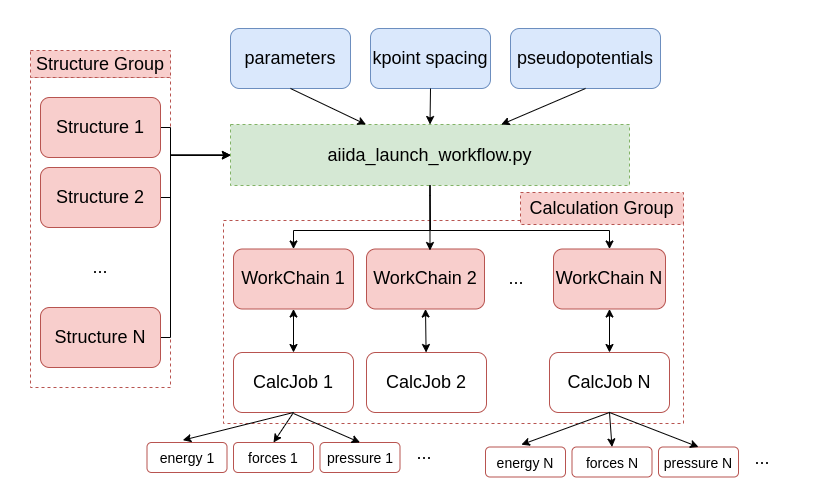
\includegraphics[width=1.0\textwidth,center]{figures/recalculateDBschematic.png}%
\caption{Schematic of AiiDA usage}%
\label{fig:aiida_methods}
\end{figure}

\section{Results and Discussion}

\subsection{Test and Training Errors}

As mentioned in the methodology, we trained 50 NNPs, with 90\% of the structures set for training and 10\% set for testing.
Figure \ref{fig:rsme_plot} shows the errors in both the testing and training samples for a single NNP.
Here we have chosen to demonstrate the results for the NNP with the lowest C44 error in pure Aluminum, but the general trends hold for all NNPs we computed. We examine the root mean square error (RMSE) for all structures $i$.
\begin{equation}
    RMSE = (\sum_i (E^{DFT}_i - E^{NNP}_i)^2)^\frac{1}{2}
\end{equation}
We see that the testing error is much larger than the training error.
However, this large error is primarily due to a single outlier, as can be seen in  Figure \ref{fig:rsme_plot}.
Removing this massive outlier lowers the testing error from 26.5 meV/atom to 3.46 meV/atom.
The outlier structure in question is for Al under massive compression, $a_0$ = 3.27$\AA$.
For our purposes, the mechanical properties of Aluminum alloys, we can consider this being beyond the compression range we would be interested in for almost all applications.
In general, the NNP breaks down at compressions beyond $\frac{a}{a_0} ~= 0.8$, as can be seen in by the plots in section \ref{sct:eos_data} in the supplementary material. 

\begin{figure}[H]%
\centering%
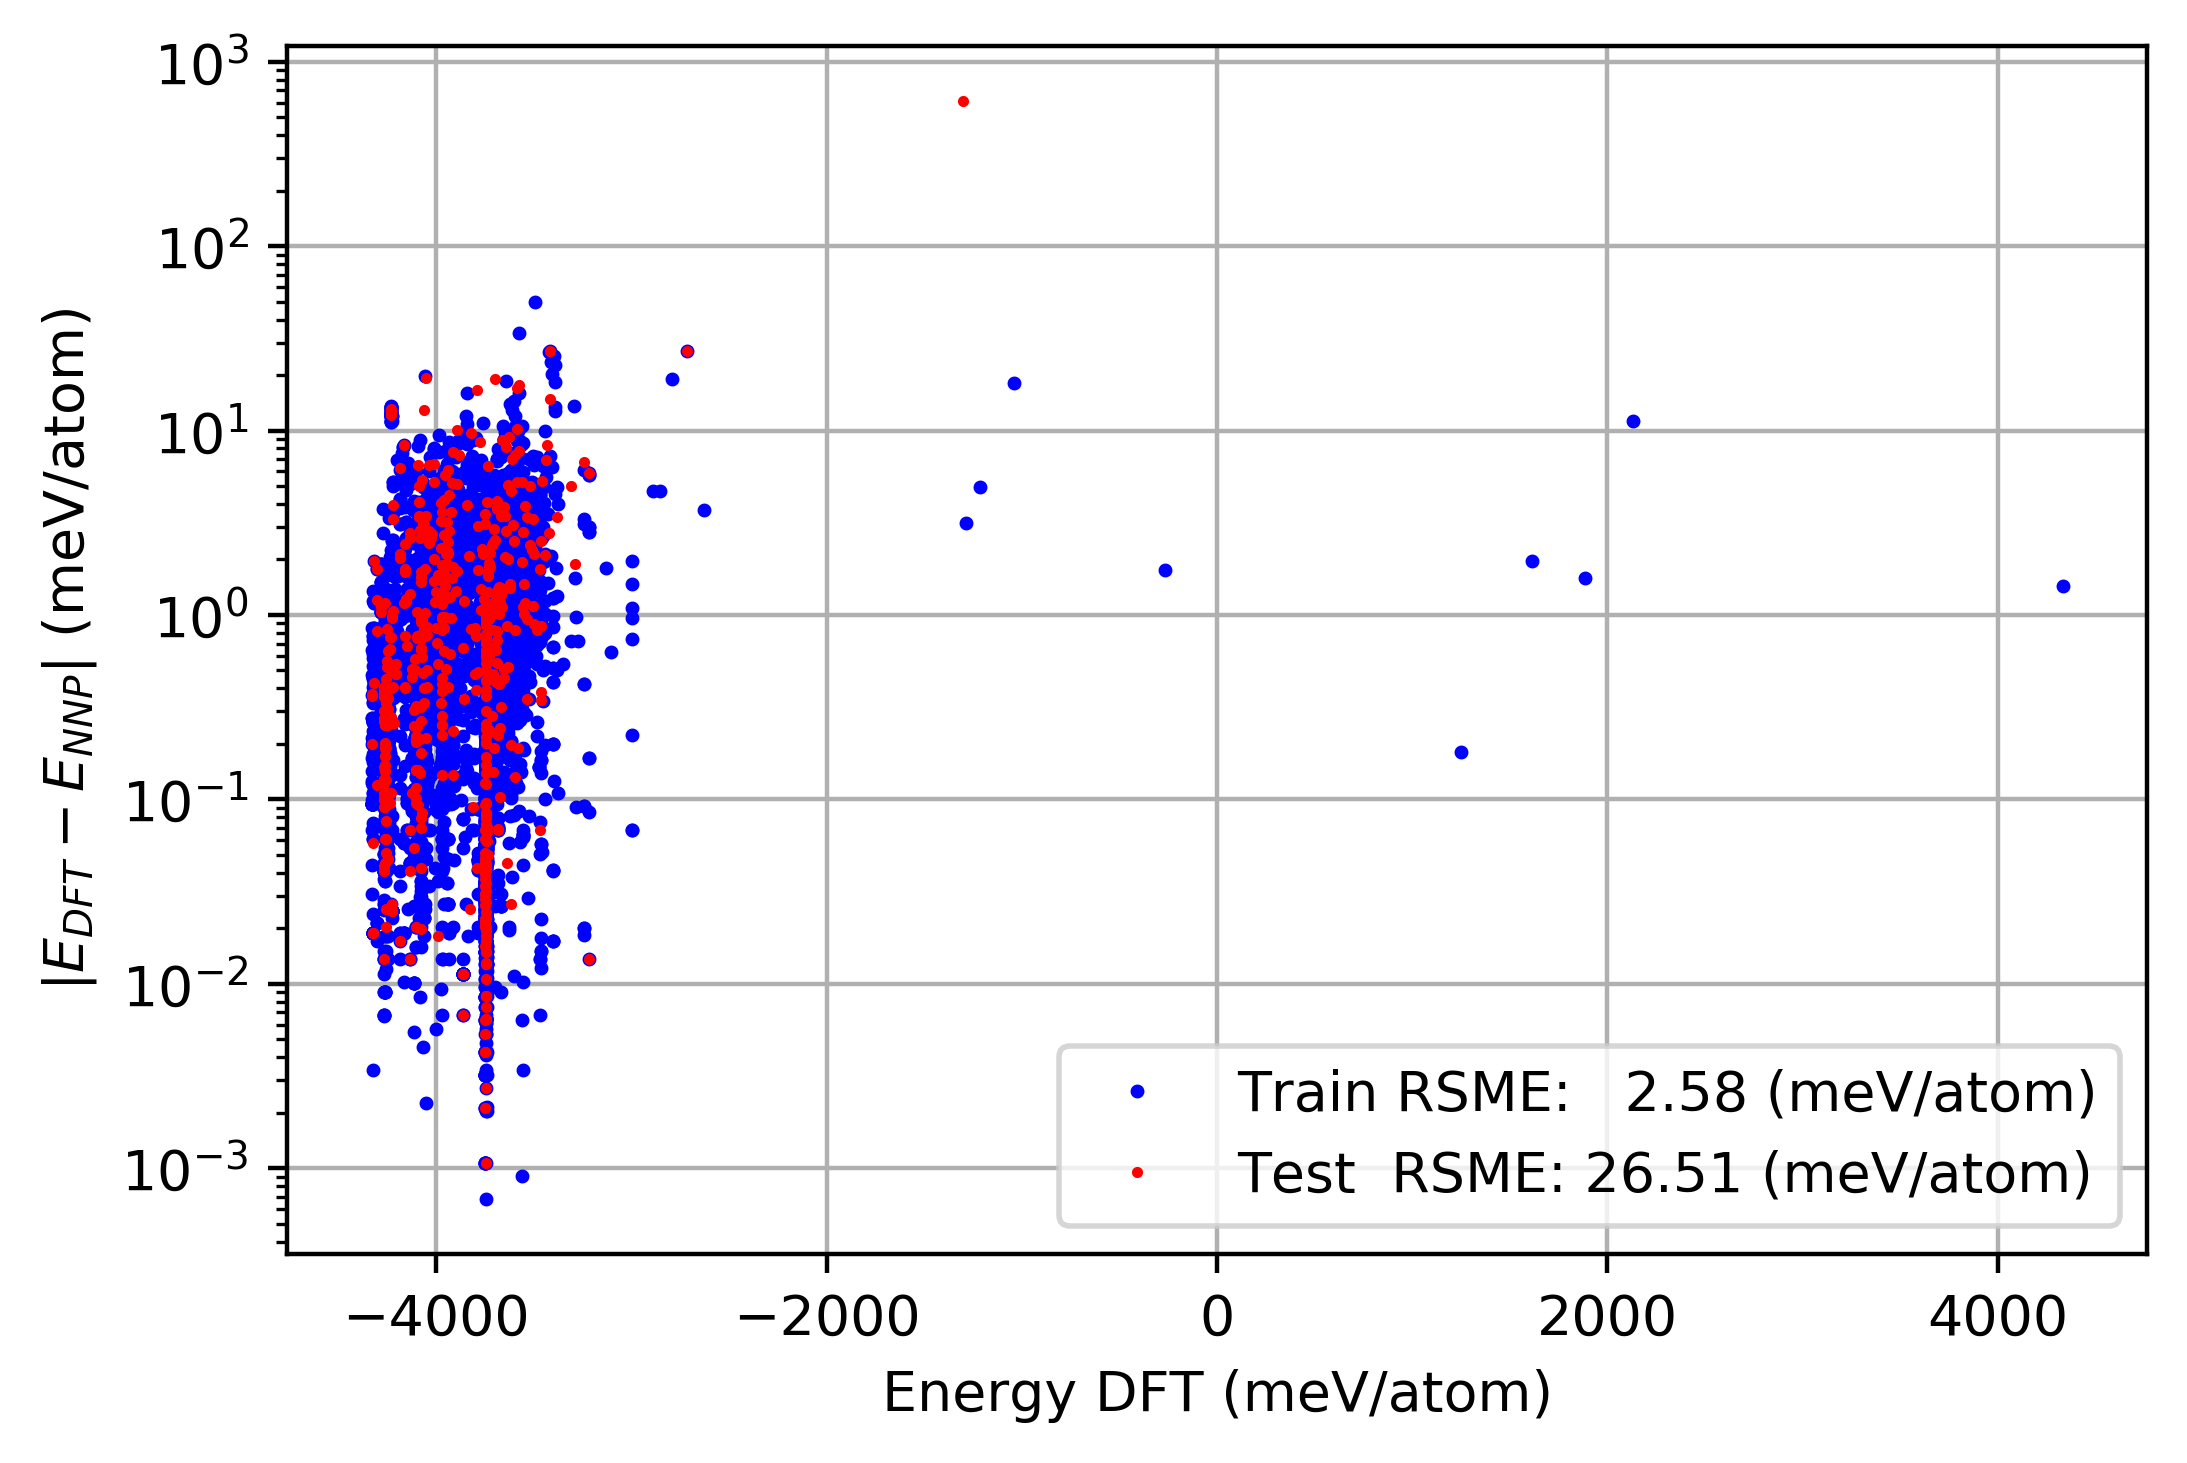
\includegraphics[width=1.0\textwidth,center]{figures/plot_nnperrors.png}%
\caption{Plot of test and training errors for NNP.
Note the large test error outlier, an order of magnitude larger than the next-greatest test error. }%
\label{fst error ig:rsme_plot}
\end{figure}

\subsection{Bulk Properties}

Figure \ref{fig:matparam_purestats} shows the performance of NNP and ADP against DFT on fundamental properties: lattice and elastic constants, surface and stacking fault energies, for pure Al and Cu.
For most of these properties, NNP shows little or no advantage relative to ADP, the sole exception being stable stacking fault energies in aluminum.
Troublingly, the $C_{44}$ values of aluminum are substantially and statistically different from those of DFT.
This error is not entirely unusual for NNPs, and prior work has found errors of a similar magnitude\cite{Zuo2020APotentials}.
On theoretical grounds, elastic constants are a function of the second derivative of energy, and one should expect to be correspondingly much harder to accurately model when training primarily on energies.
Because we have used a very dense kpoint mesh, and we have systematically used the same settings, we do not expect this error in $C_{44}$ to be due to issues in the underlying training set, as was found to be a critical factor for a machine-learning we potential based on iron \cite{Dragoni2018AchievingIron}.  
In any case, we find that our potential is highly performant when one is considering a broad range of structures, or when one is evaluating energetics of complex geometries. 

\begin{figure}[H]%
\centering%
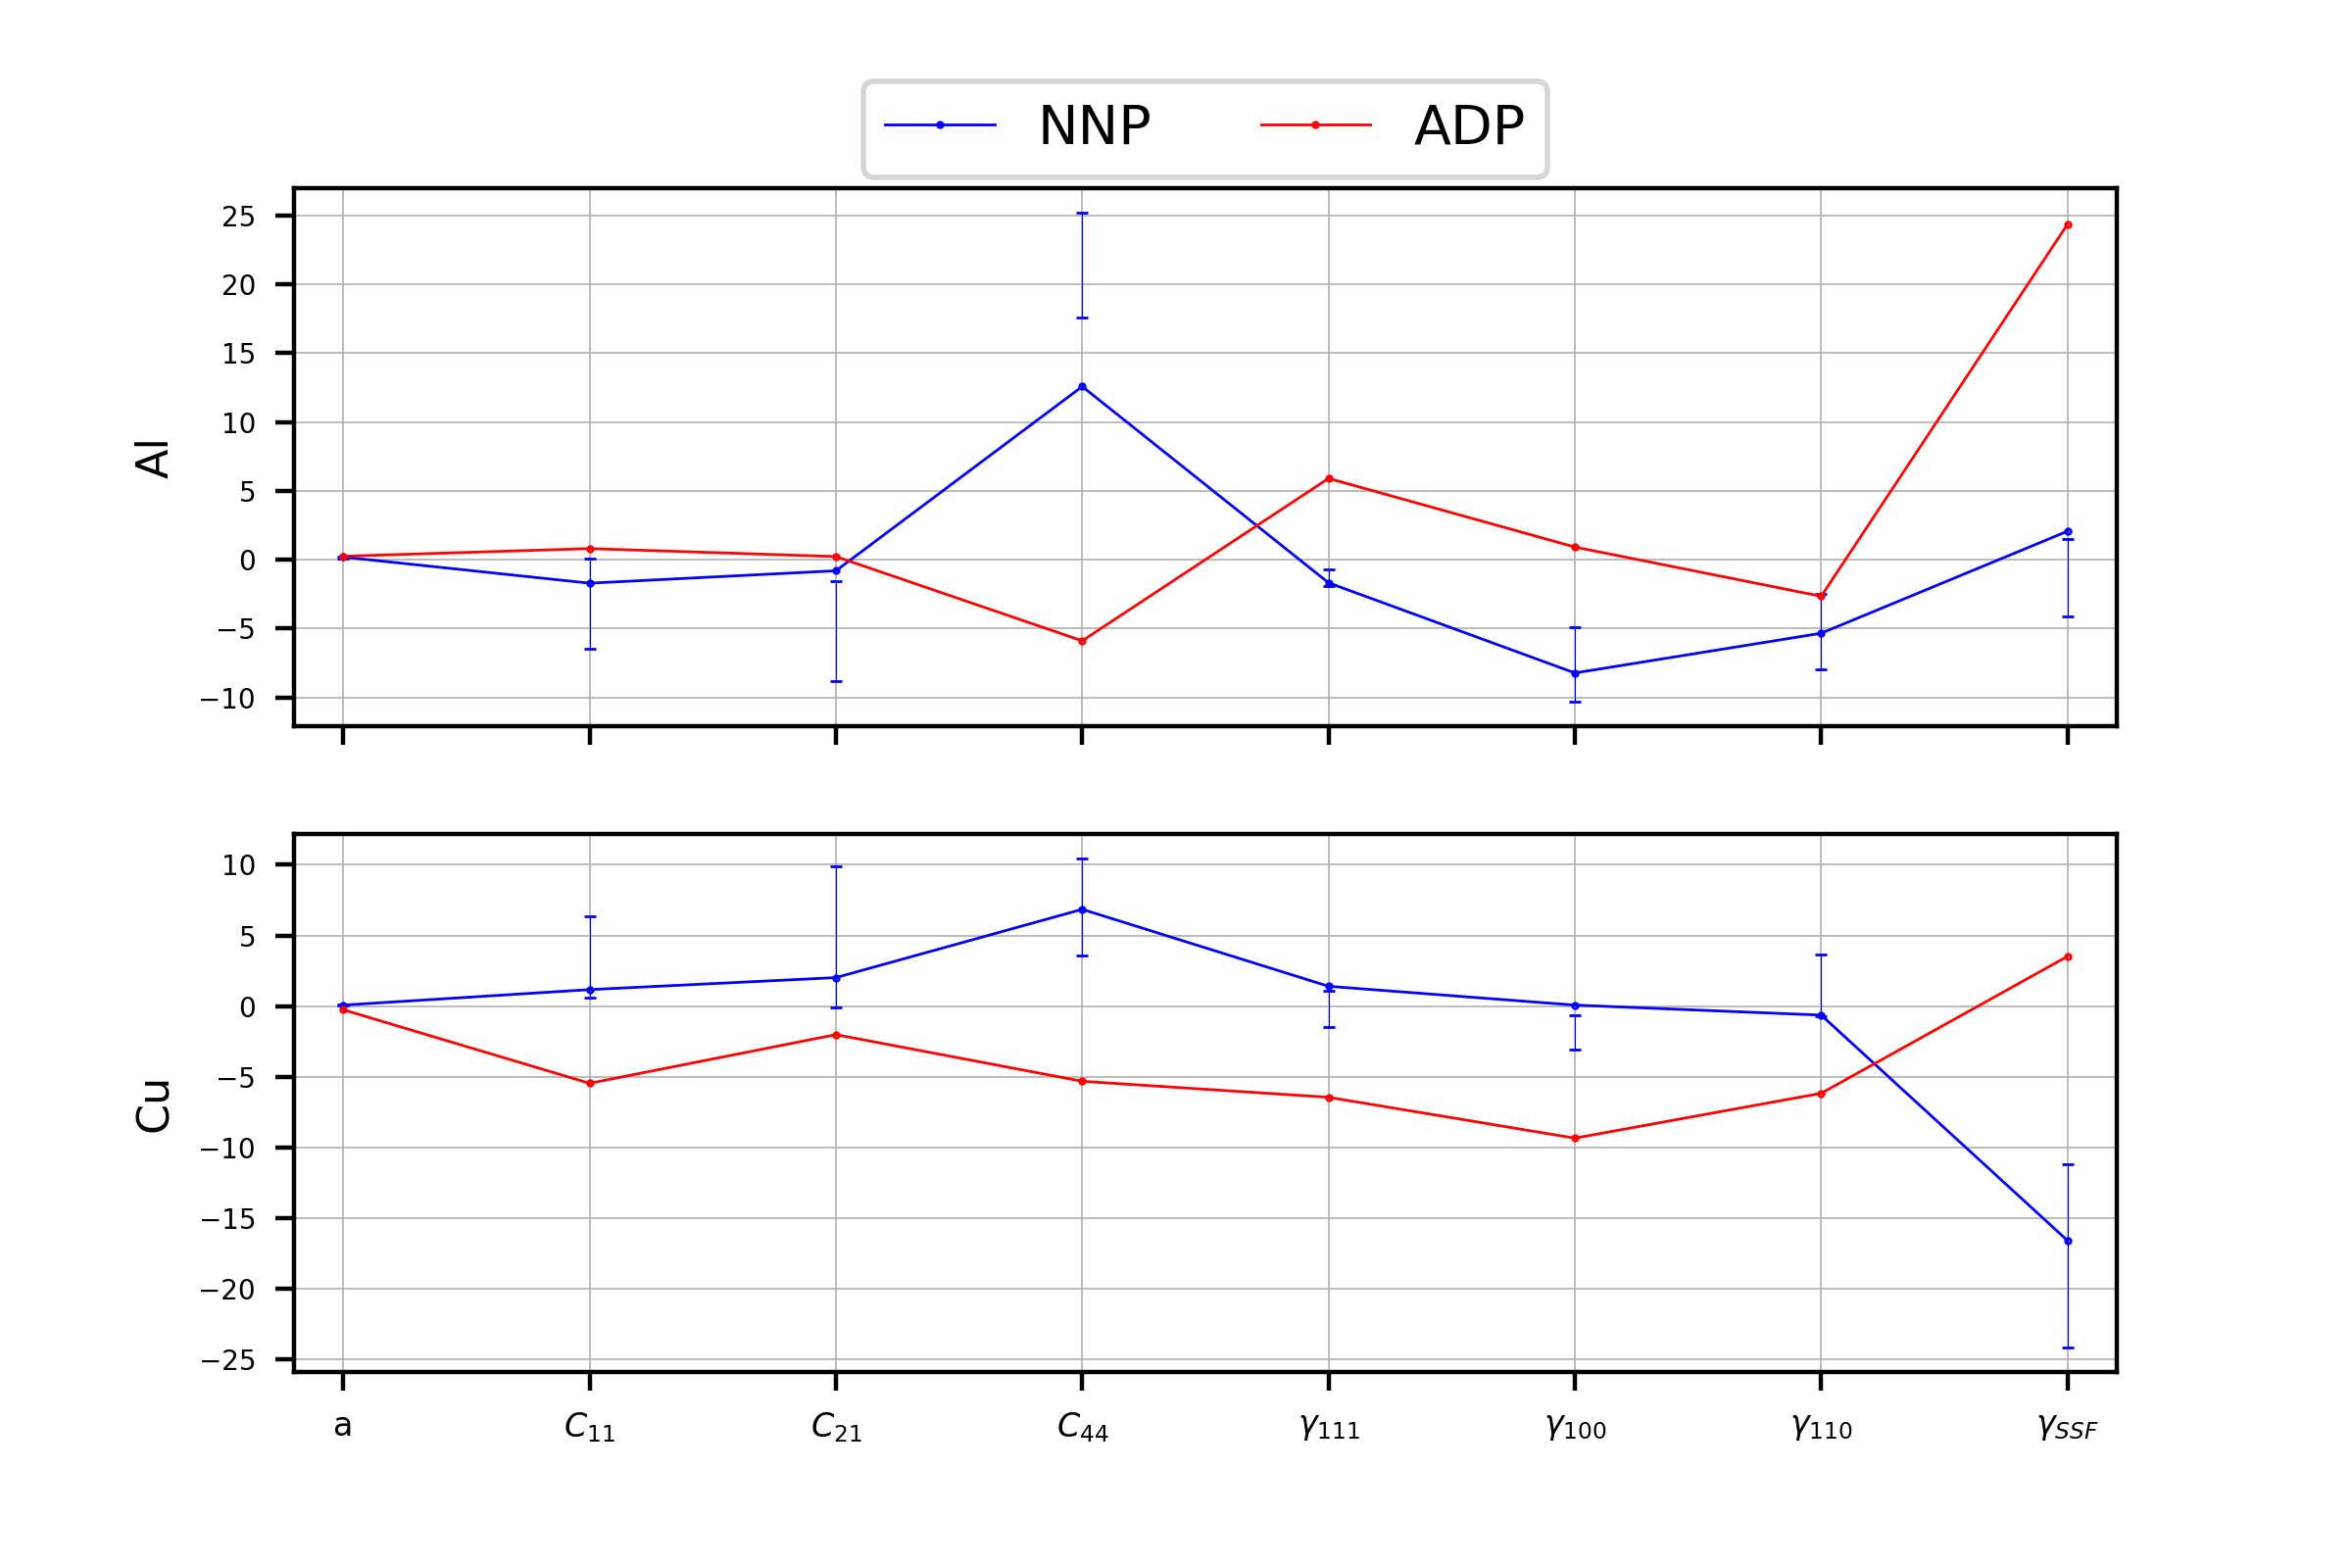
\includegraphics[width=1\textwidth,center]{./figures/matparam_purestats.png}%
\caption{Deviation of NNP and ADP from DFT (\%) for fundamental properties for Al and Cu. 
Relevant structures are included in the training set. }%
\label{fig:matparam_purestats}
\end{figure}
All the Al-Cu structures in the OQMD were evaluated for this potential, as described previously in the methodology.
The NNP outperforms ADP for formation energy, atomic volume, and elastic constants for most OQMD structures, as can be seen in Figure \ref{fig:matparam_stats1}.
We compute structure formation energy $\Delta E^{structure}_f$ of all structures,
, as relative to bulk FCC Al and dilute Cu in matrix:
\begin{equation} \label{eqn:formE_structure}
\Delta E^{structure}_f = E^{structure}_N - nE^{ref}_Al-(N-n)E^{ref}_{Cu}
\end{equation}
\begin{equation} \label{eqn:formRef_Al}
E^{ref}_{Al} = E^{FCC}_{Al}
\end{equation}
\begin{equation} \label{eqn:formRef_Cu}
E^{ref}_{Cu} = E^{1sol}_{255Al,1Cu} - 255E^{FCC}_{Al}
\end{equation}
Where, for a given structure, $N$ is the total number of atoms, $n$ is the number of Al atoms, and $N-n$ the number of Cu atoms. Formation energy is particularly well-handled by the NNP, with most errors well within a few meV/atom, while ADP often highly overestimates or underestimates the formation energy;
in a few cases, ADP reverses the sign, i.e., predicting stable compounds as unstable and vice versa.
However, for structures with high formation energy, both the NNP and ADP tend to struggle, often they do not end up relaxing to the same structure as DFT, or they have substantial errors.
ADP regularly underestimates the atomic volume, even for critical structures: $\theta$ and $\theta'$ errors can be substantial.
For elastic constants, we see that neither ADP nor NNP perform ideally.
ADP does a reasonable job of capturing the precipitate structures and outperforms NNP on pure aluminum.
However, we see that ADP often makes quite substantial errors in the elastic constants for intermediate compounds, while this is less the case for NNP. Interestingly it seems that the B2 structure poses a challenge to both ADP and most NNP.
ADP predicts B2 to be extremely stable, while it has the highest error for any stable compound for NNP. 


\begin{figure}[H]%
\centering%
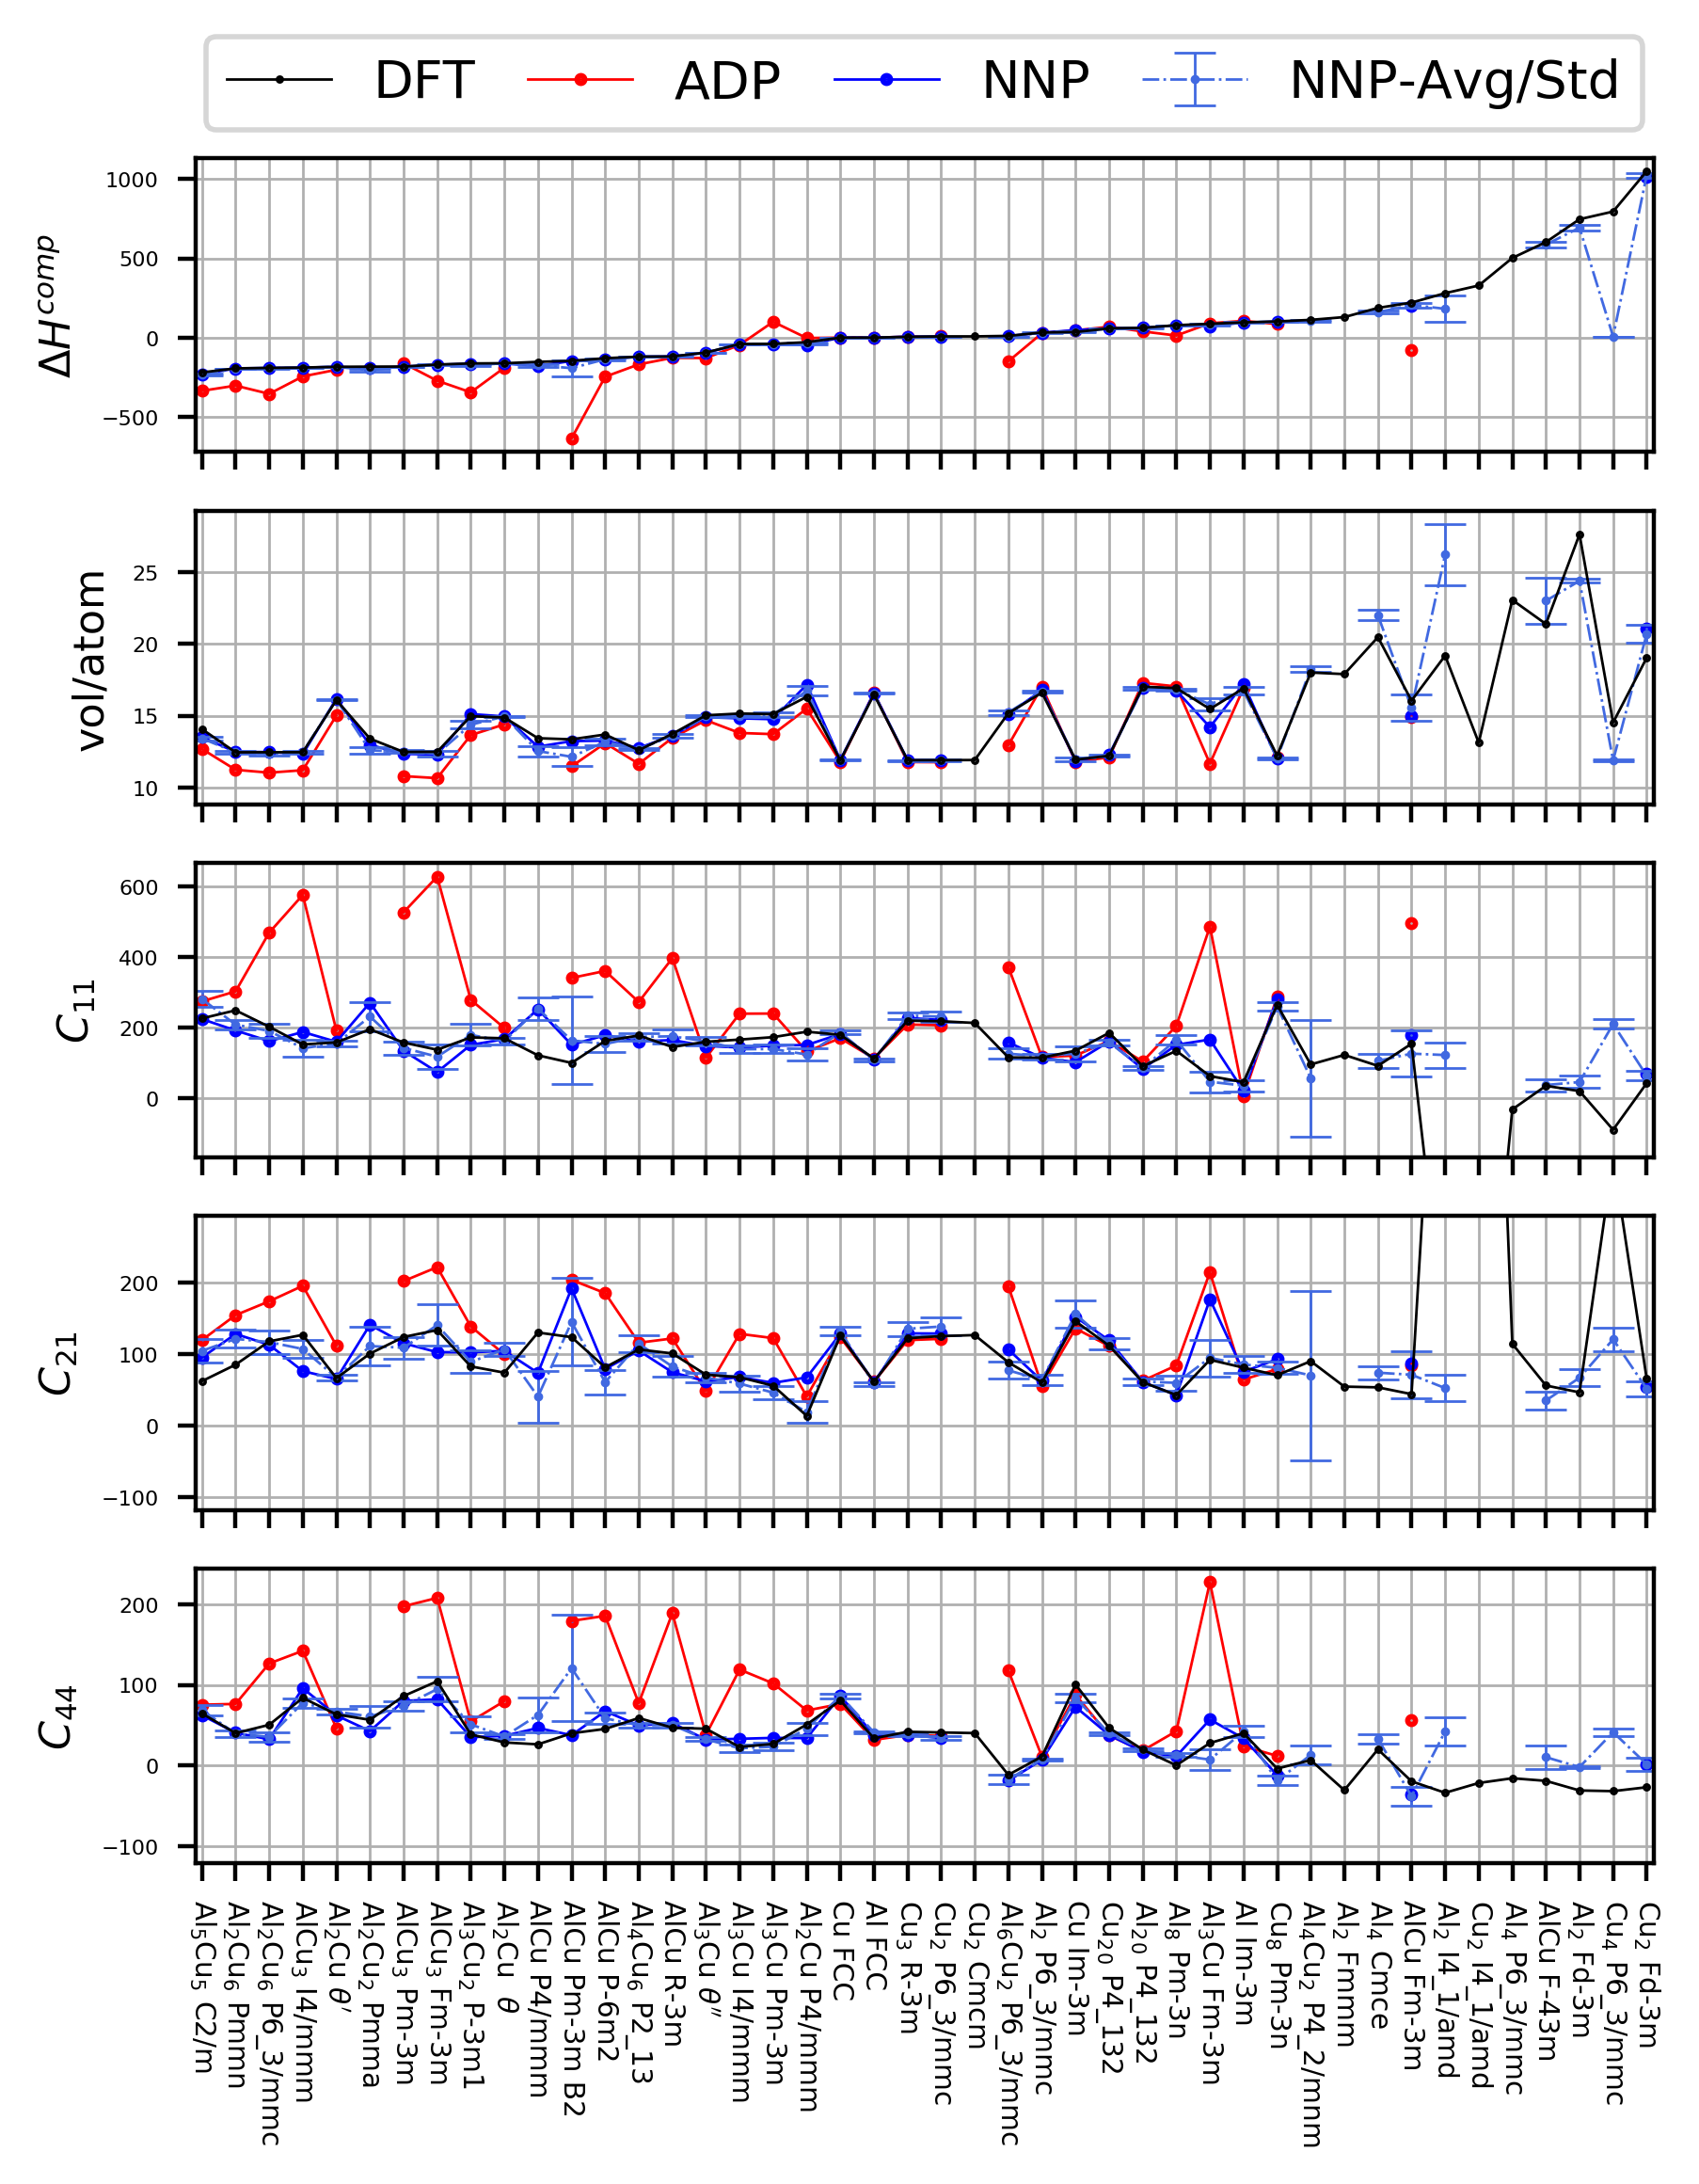
\includegraphics[width=1\textwidth,center]{figures/matparam_stats1.png}%
\caption{Comparison of: formation energy (meV), atomic volume (Ang$^3$), elastic constants C$_{11}$, C$_{21}$ and C$_{44}$ (GPa) across NNP, ADP and DFT for all structures in the OQMD. 
Relevant structures are included in the training set. }
\label{fig:matparam_stats1}
\end{figure}

\subsection{Solutes}
The binary formation energies for Cu, Al, and Vacancy in Al or Cu matrix was computed with following:
\begin{equation}
\Delta E^{bind}_f = E^{2sol}_{N-2,X,Y}-E^{1sol}_{N-1,X}-E^{1sol}_{N-1,Y}+E^{pure}_N
\end{equation}
Note for Al-matrix results this is the same as equation \ref{eqn:formE_structure}, while for 
Cu-matrix results the reference is swapped to Cu matrix and Al solute.
Also, due to Cu having a much higher computational cost, reference is to a 108 atom 3x3x3 supercell.
The results for Al matrix are displayed in Figure \ref{fig:solsol_in_al} while those for Cu matrix are contained in the \textcolor{red}{Figure S \ref{fig:solsol_in_cu}}.
For the solute binding, we see that the NNP, while not always ideal, more closely matches DFT than ADP.
Particularly for dilute Cu-Cu binding, ADP falsely predicts massive overbinding for near neighbors and massive repulsion for further neighbors, while NNP maintains quantitative accuracy.
Errors for NNP are typically in the 20-30 meV range.


\begin{figure}[H]%
\centering%
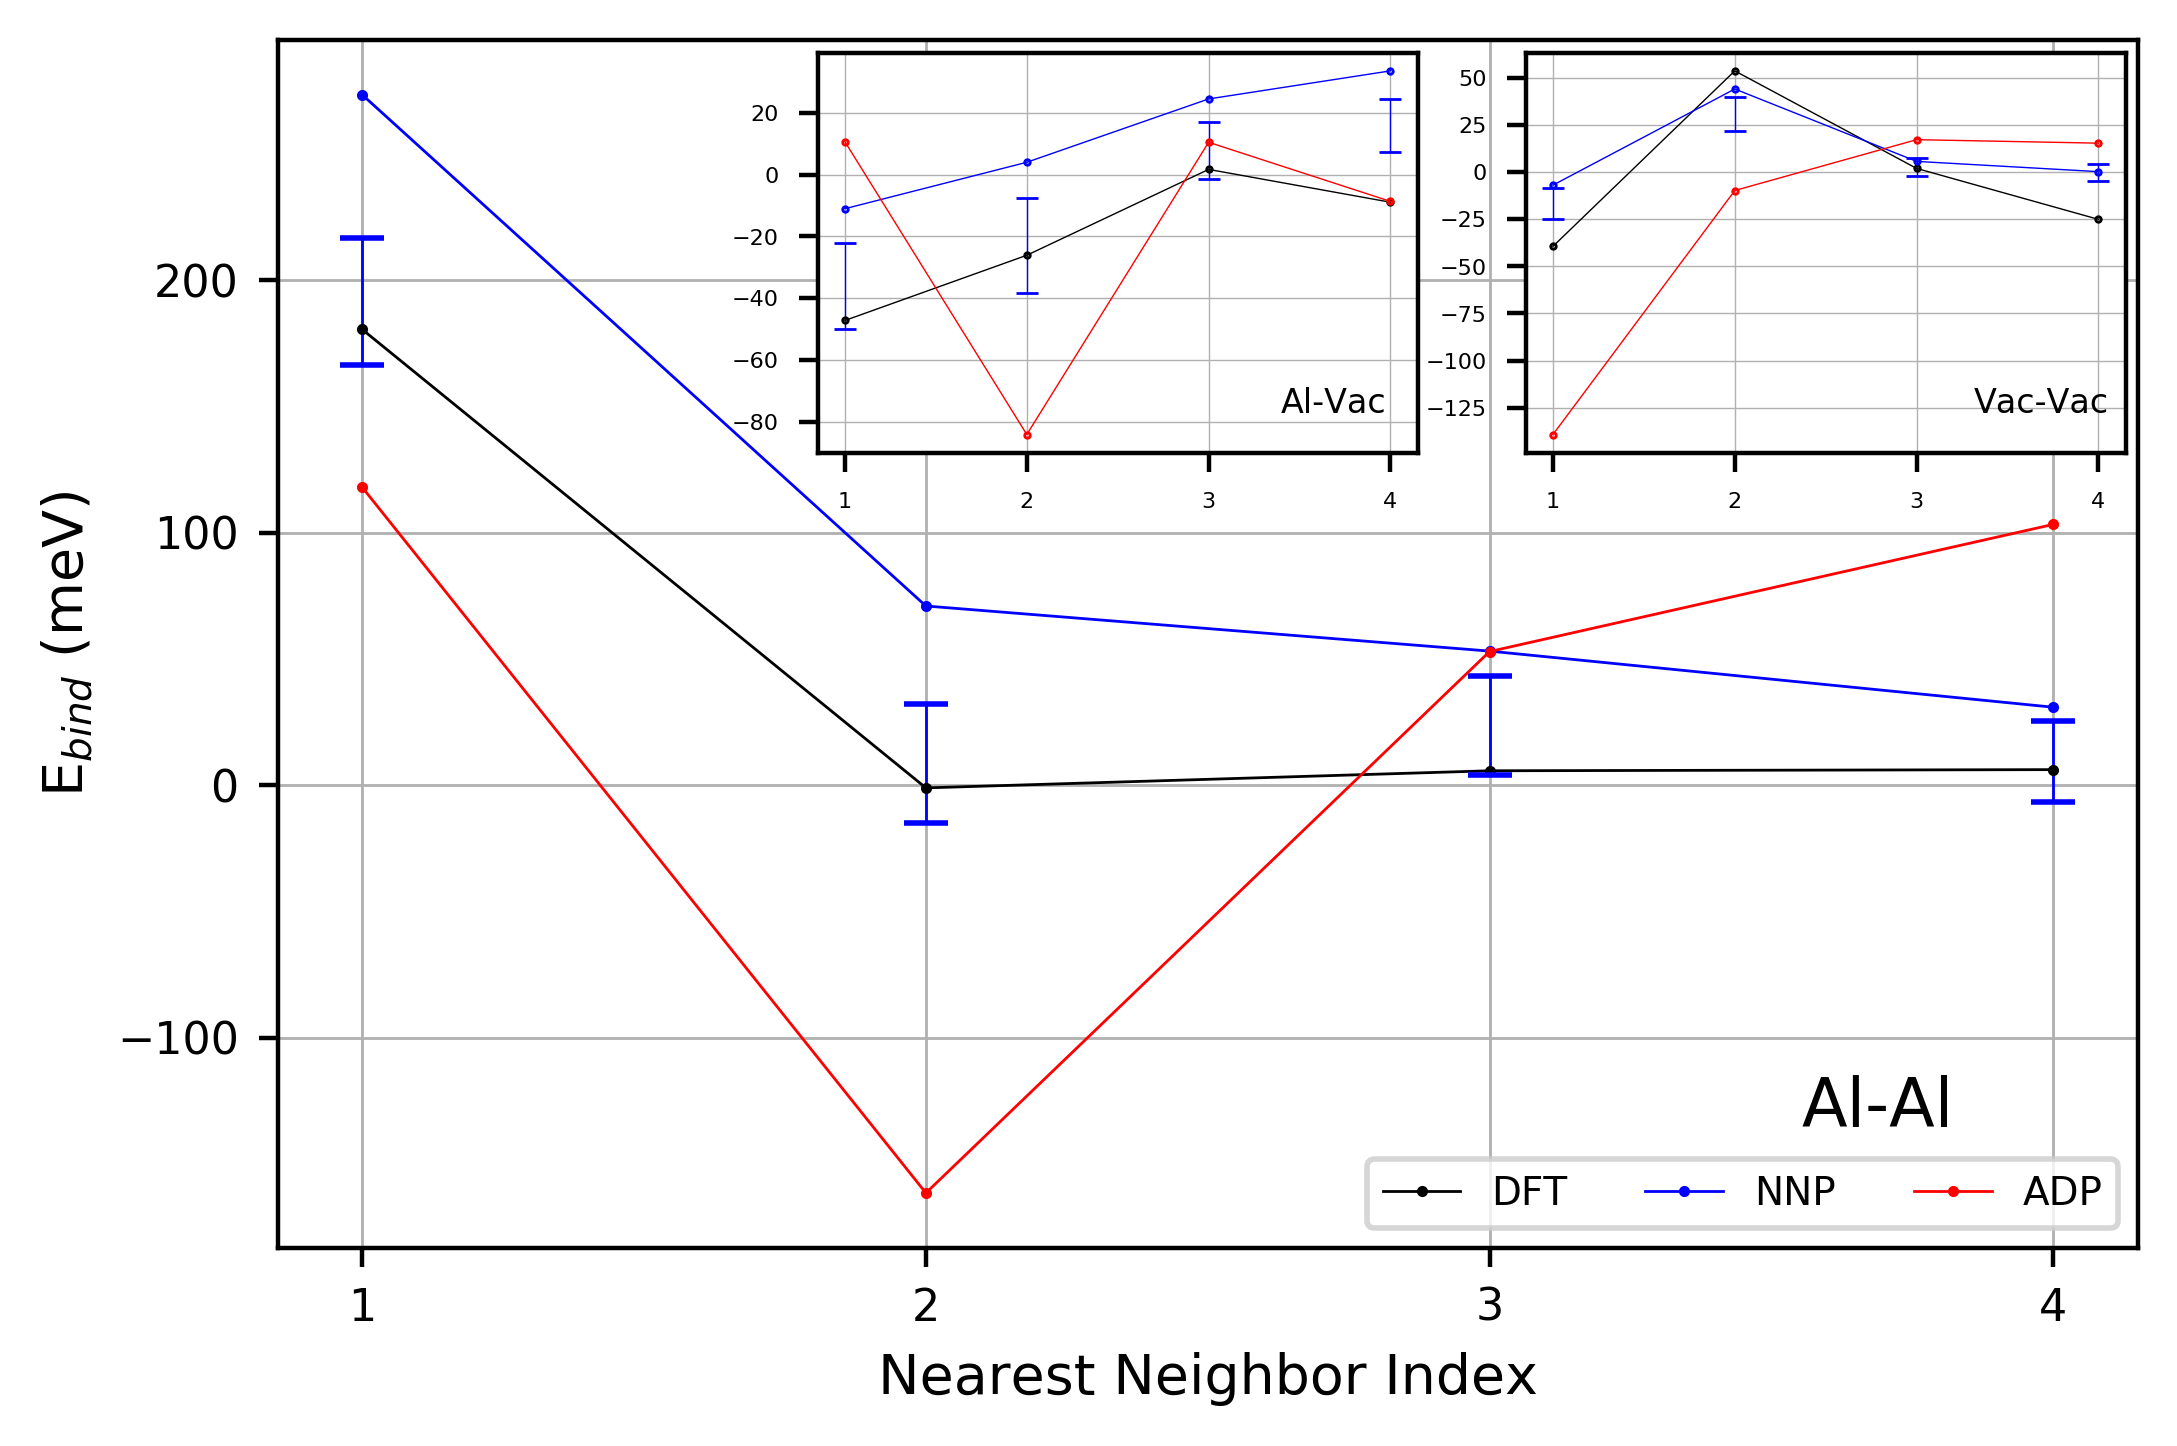
\includegraphics[width=1\textwidth,center]{./figures/solsol_in_al.png}%
\caption{Neighbor index vs. binding energy $E_{bind}$ for Cu-Cu, Cu-Vac and Vac-Vac in Al matrix. 
Relevant structures are included in the training set.}%
\label{fig:solsol_in_al}
\end{figure}


In Table \ref{table:solute_special}, we report further properties of dilute solutes: 3 and 4 atom clusters, misfit volume, and solute-stacking fault interactions.
Firstly we extend the binary results to simple clusters of 3 and 4 atoms, and compute the cluster formation energy, $\Delta E^{cluster}_{f,(N-X,X)}$,
in the same manner as in Equation \ref{eqn:formE_structure}, which we make explicit below:

\begin{equation}
\Delta E^{cluster}_{f,(N-X,X)} = E^{cluster}_{N-X,X} - \sum_i E^{ref}_i
\end{equation}

The superscript defines the cluster by describing the neighboring indexes, same as in \cite{Gorbatov2019EffectiveAlloys}.
These results cover the same clusters that were examined by Gorbatov et al. .\cite{Gorbatov2019EffectiveAlloys}, with which they were able to produce GP-I and GP-II zone formation in a cluster-expansion model.
We note that the 111 and 111111, namely a compact triangle and tetrahedral of nearest neighbors respectively, are not compatible with the (100) plane formation that characterizes GP-I and GP-II zones, while the 111112 and 111122 clusters are.
Naturally, we then find that the (100) plane-favoring clusters are energetically preferable, while the (100) plane incompatible clusters are not.
We see that ADP gets the absolute values wrong, predicting all clusters as being overly stable; it also gets the relative trends of the 3-atom clusters wrong.
Our selected NNP also flips the 111 and 112 cluster atom stability, but otherwise is in good agreement with relative trends and absolute values of cluster formation energies.
Importantly, we see that the average NNP performs much better than our selected NNP, and we can choose several NNPs that can have excellent performance for this property. 
We evaluated misfit volume by manually relaxing matrix with the solute present for ADP and the NNPs, and by computing directly from the pressure and bulk modulus of a solute-containing cell for DFT.
We see that ADP contains gross errors, with a massive massively negative error for Cu in Al, and reversing the sign of Cu in Al (predicting a positive misfit volume, rather a negative one).
Most NNPs, including our selected NNP, attain reasonable accuracy for this value, within ~2$\AA^3$ of the DFT value. 
Solute-dislocation interaction energies are vital when considering solute strengthening\cite{Leyson2010}.
We computed solute-stacking fault energy, $E^{Sol-SF}_{f,(N-1,X)}$, as a proxy parameter in the manner described in\cite{Yin2017a}.
Namely, we computed:

\begin{equation}
\Delta E^{Sol-SF}_{f,(N-1,X)} = E^{Sol-SF}_{N-1,X} - E^{SF}_{N} - (E^{Pristine}_{N-1,X}-E^{Pristine}_{N})
\end{equation}

Where $E^{Sol-SF}_{N-1,1}$ is the energy of a stacking fault with a single solute,
$E^{SF}_{N}$ is the energy of a stacking fault,
$E^{Pristine}_{N-1,X}$ is the energy of single solute in a pristine matrix (of the same size as the SF cell), 
and $E^{Pristine}_{N}$ the energy of pristine matrix. 
The results show that both potentials have good results (within ~50meV of DFT value).
The NNP showing better accuracy for Cu in the Al matrix and ADP shows better results for Cu in the Al matrix.


\begin{table}[h!]
\begin{tabular}{l|cccc}%
\hline%
&DFT&ADP&NNP& NNP-\emph{Avg / StdDev}\\%
\hline%
$E^{3Cu}_{111}$ (eV)&-0.073&{-}0.718&{-}0.112&\emph{-0.060 / 0.037}\\%
$E^{3Cu}_{112}$ (eV)&-0.112&{-}0.595&{-}0.097&\emph{-0.085 / 0.025}\\%
$E^{4Cu}_{111111}$(eV)&0.039&{-}0.612&{-}0.081&\emph{0.071 / 0.086}\\%
$E^{4Cu}_{111112}$(eV)&-0.126&{-}1.071&{-}0.184&\emph{-0.093 / 0.066}\\%
$E^{4Cu}_{111122}$(eV)&-0.268&{-}1.275&{-}0.226&\emph{-0.205 / 0.055}\\%
Misfit Vol Cu in Al ($\AA^3$)&{-}5.770&{-}16.958&{-}4.380&\emph{-7.095 / 1.076}\\%
Misfit Vol Al in Cu ($\AA^3$)&2.421&{-}1.259&0.109&\emph{1.334 / 0.857}\\%
SolSF Cu in Al (eV)&0.052&0.108&0.042&\emph{0.062 / 0.030}\\%
SolSF Al in Cu (eV)&{-}0.049&{-}0.034&{-}0.006&\emph{0.002 / 0.031}\\%
\end{tabular}%
\caption{Misfit Volumes, Cu cluster energies and solute-stacking fault interactions for DFT, ADP and NNP. 
The 3 and 4 body clusters and not explicitly included in the training set, while the Misfit Volume and 
Solute-Stacking fault structures are.}
\label{table:solute_special}
\end{table}

\subsection{Interfaces}
In this work, the coherent and semicoherent versions of the $\theta''$ and $\theta'$ interfaces were studied while $\theta$ was omitted since it only forms incoherent interfaces \cite{Nie2014PhysicalAlloys}.
We constructed these interfaces by taking their OQMD entries and stacking them on the Al matrix using the ASE \mintinline{python}{ase.build.stack} command.
During relaxation, atoms are free to move, but the cell is held fixed. 

We computed the interface energy in the same manner as in \cite{Vaithyanathan2004MultiscaleAlloys}, and we only briefly summarize the method here.
The formation energy for an interface with N atoms of which X are of the matrix and Y are of the precipitate,
$\Delta E^{interface}_{f, (X,Y)} = E^{interface}_{X,Y}-XE^{Matrix}_{bulk}-YE^{Precip}_{bulk}$,
is related to the number of atoms in the following equation. 
\begin{equation}
\Delta E^{interface}_{f,(X,Y)} = \delta E^{strain}_{X,Y} + \frac{2A\gamma^{interface}}{N}
\end{equation}
Where $\Delta E^{interface}_f$ is the interface formation energy, $\delta E_{strain}$ is the strain energy, $A$ the surface area,
$\gamma^{int}$ the interface energy, and $N=X+Y$ the total number of atoms in interface.
The interface surface energy $\gamma^{interface}$ is then the slope of $\frac{1}{N}$ against
$\Delta E^{interface}_f$, divided by $2A$.
We calculated the slope using three different sizes of the $\theta'$ structures and four different sizes of $\theta''$ structures, starting with a minimum of one precipitate layer and two Al layers and incrementing onward in size. 




Figure \ref{fig:interface_energies} plots the results of the interface energy calculations.
ADP correctly predicts the general trends but makes several serious errors.
The coherent $\theta'$ interface has much too high an energy, while all the $\theta''$ interface is predicted to have negative energy.
The $\theta''$ interface is particularly challenging because it has such low interface energy; therefore, it is easy for the potential to predict this to be negative rather than positive.
However, our representative NNP has high quantitative accuracy on all these interfaces.

\begin{figure}[H]%
\centering%
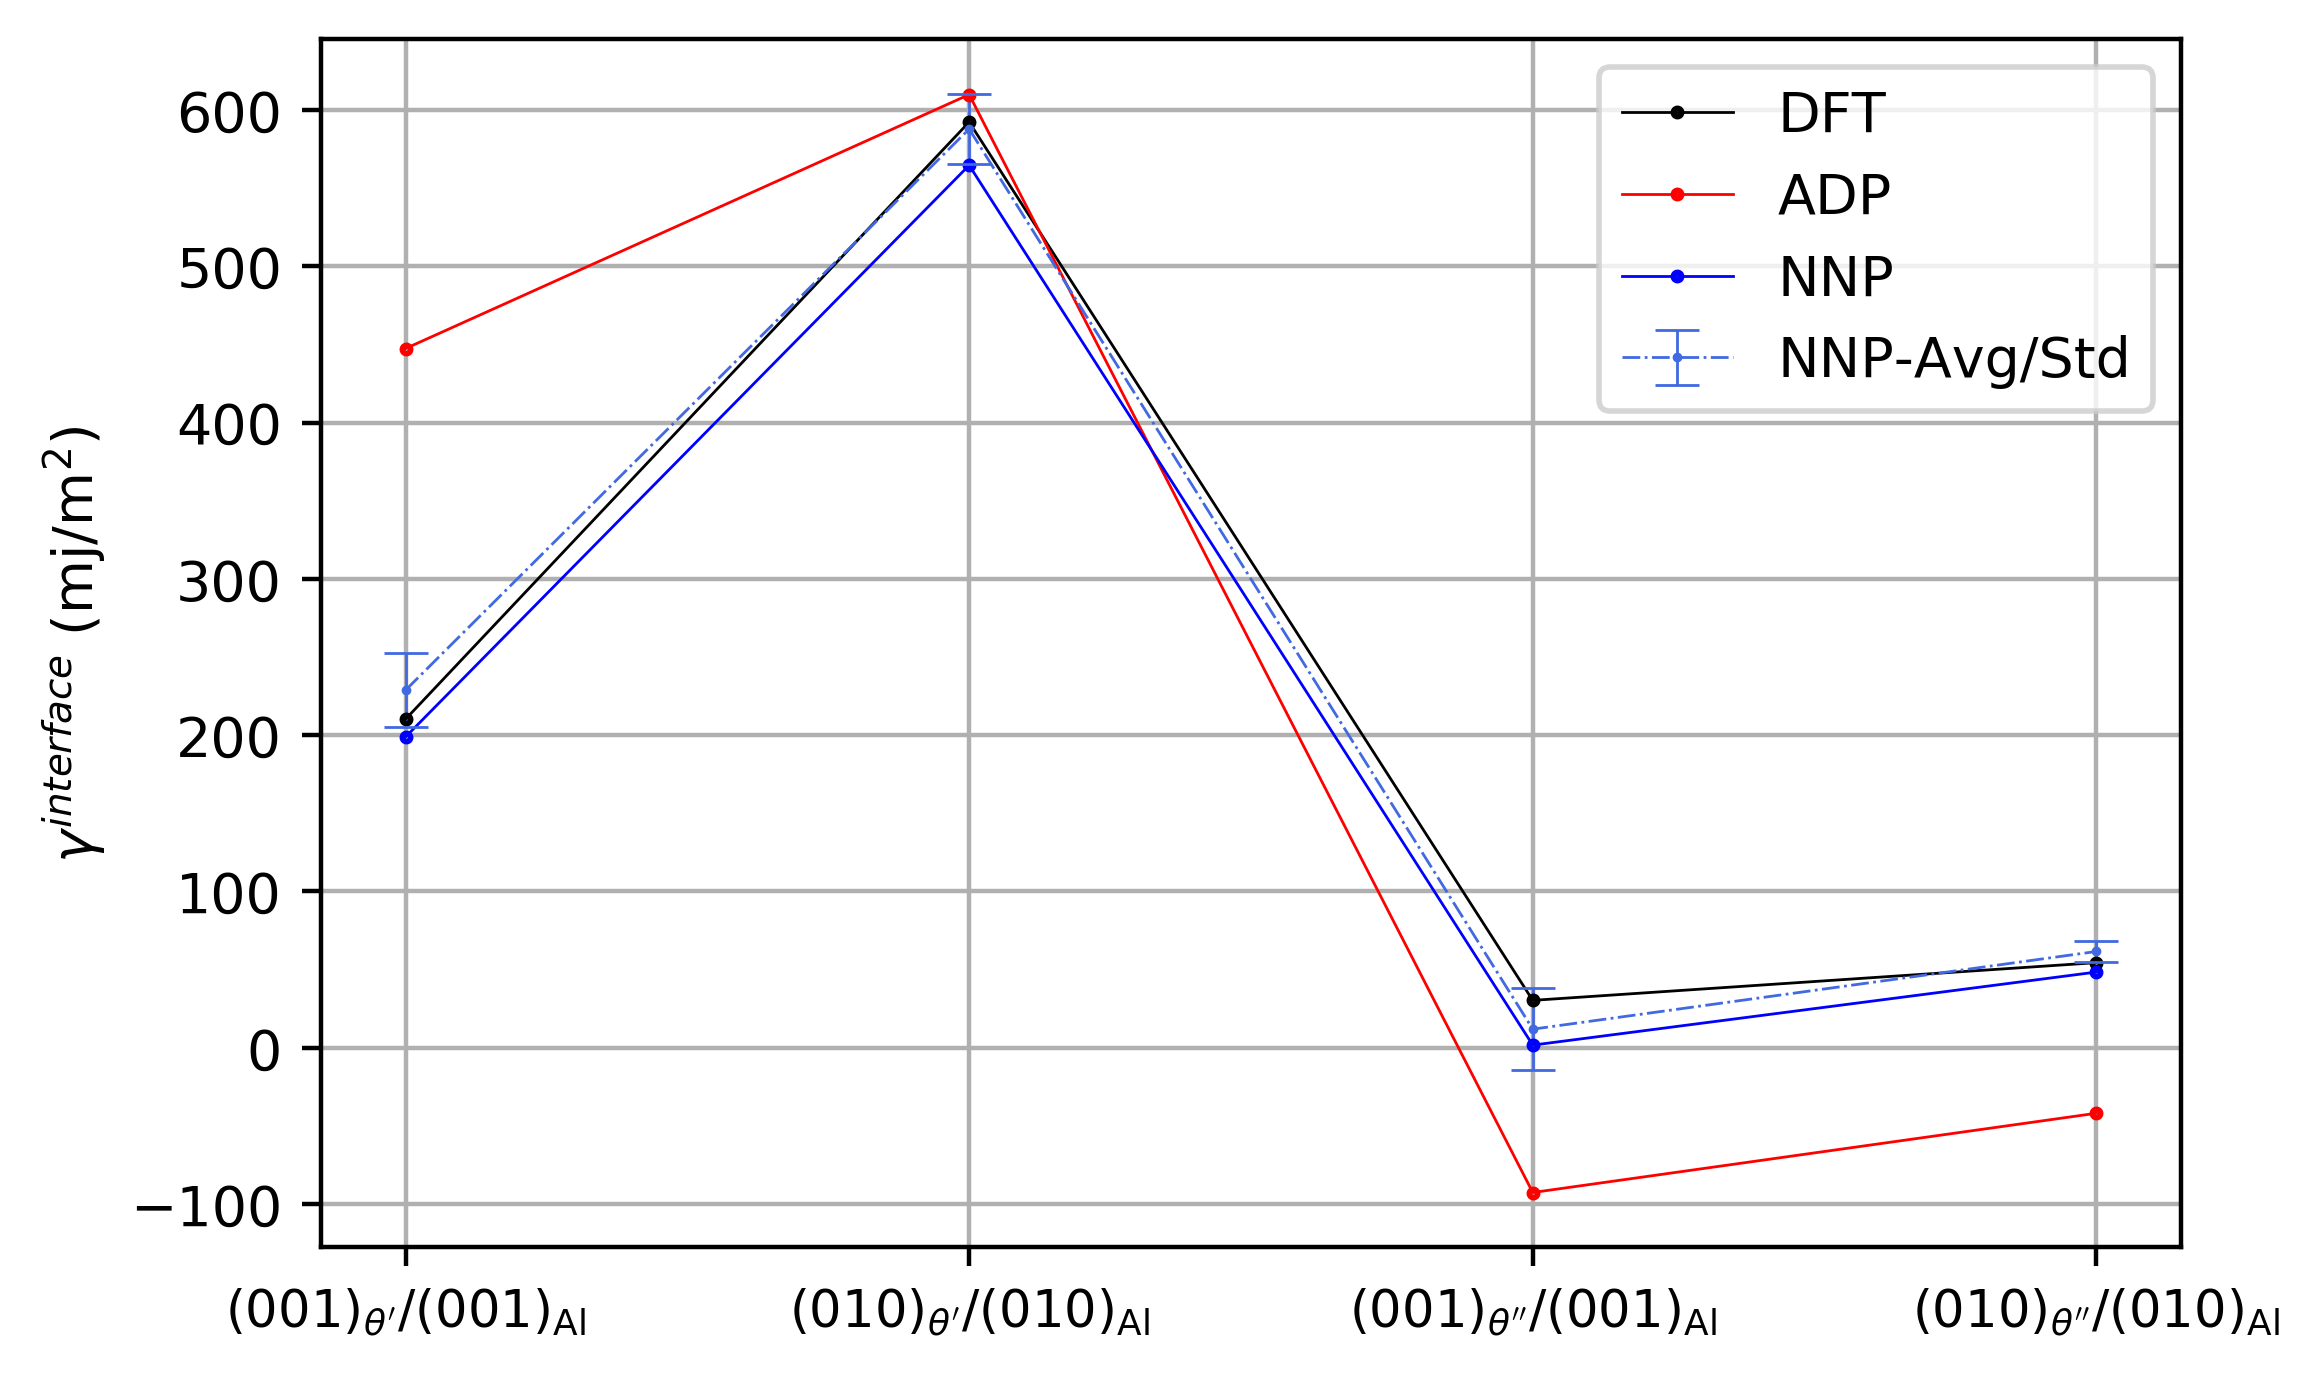
\includegraphics[width=1\textwidth,center]{./figures/interface_energies.png}%
\caption{Interface structure vs. interface energy for precipitate structures. 
These are the $\theta'$ coherent, $\theta'$ semi-coherent, $\theta''$ coherent and $\theta''$ semi-coherent
interfaces in order. Relevant structures are included in the t/raining set.}%
\label{fig:interface_energies}
\end{figure}

\subsection{Generalized Stacking Faults}
The most mechanically important GSF surface is that which coincides with the (111) plane of aluminum, which we display in Figure \ref{fig:GSF_ThetaDP_111} (b).
To compute the GSF energy surface (GSFE), we follow the procedure detailed in \cite{Yin2017a}, which we briefly summarize here.
Firstly, we reshape the base cell to find the smallest cell such that a1 and a2 lie on the plane of interest, with a3 going out of the plane.
Then for each point, $\vec{R}$, of the GSF the a3  cell vector was correspondingly shifted,
then both the atoms and the a3 cell vector were allowed to relax, but only in the z-direction.
The GSF energy at a displacement $\gamma_{GSF\vec{R}}$ was calculated using: 
\begin{equation}
\gamma^{GSF}_{\vec{R}} = (E^{GSF}_{\vec{R}} - E^{pristine})/A
\end{equation}
Where $E^{GSF}_{\vec{R}}$ is the total energy of the GSF displaced at $\vec{R}$, $E_{pristine}$ is the 
the energy of the pristine structure without deformation and $A$ is the area spanned by the GSF surface.
In Figure \ref{fig:GSF_ThetaDP_111} (a), we see the results for the entire GSF surface.
The NNP potential gives a smooth GSFE, with clear peaks and valleys in the energy corresponding with the underlying atomic positions.
The GSFE of the ADP potential, conversely, is substantially less smooth; there is also a noticeable lack of radial symmetry and high and low energy sites,  with sharp ridges extending across high energy regions.
Most troubling for ADP, is that regions of the $\theta''$ surface are unphysically negative in energy, this severely compromises ADP to give high-quality results for dislocation-precipitate interactions.
Importantly, NNP gives highly accurate energies, even though we did not train the NNP for this GSFE.
In Figure \ref{fig:GSF_Theta_0m11}, we detail a further example of using the NNP for evaluating a GSFE, this time for the (0$\overline{1}$1) for $\theta$ phase. 
Firstly, we see that by this time, including structures in the training set, we attain very high accuracy in the GSF energy. 
Secondly, regions without training show a smooth variation, with peaks and valleys in energy that correspond to the atomic structure, conversely, ADP has multiple sharp shifts in the GSFE, which appear to be artifacts.  Thus we see that NNPs can accurately scout the GSFE, and we can improve them by including a few DFT structures if needed. 

\begin{figure}[H]%
\centering%
\subfloat[]{{
 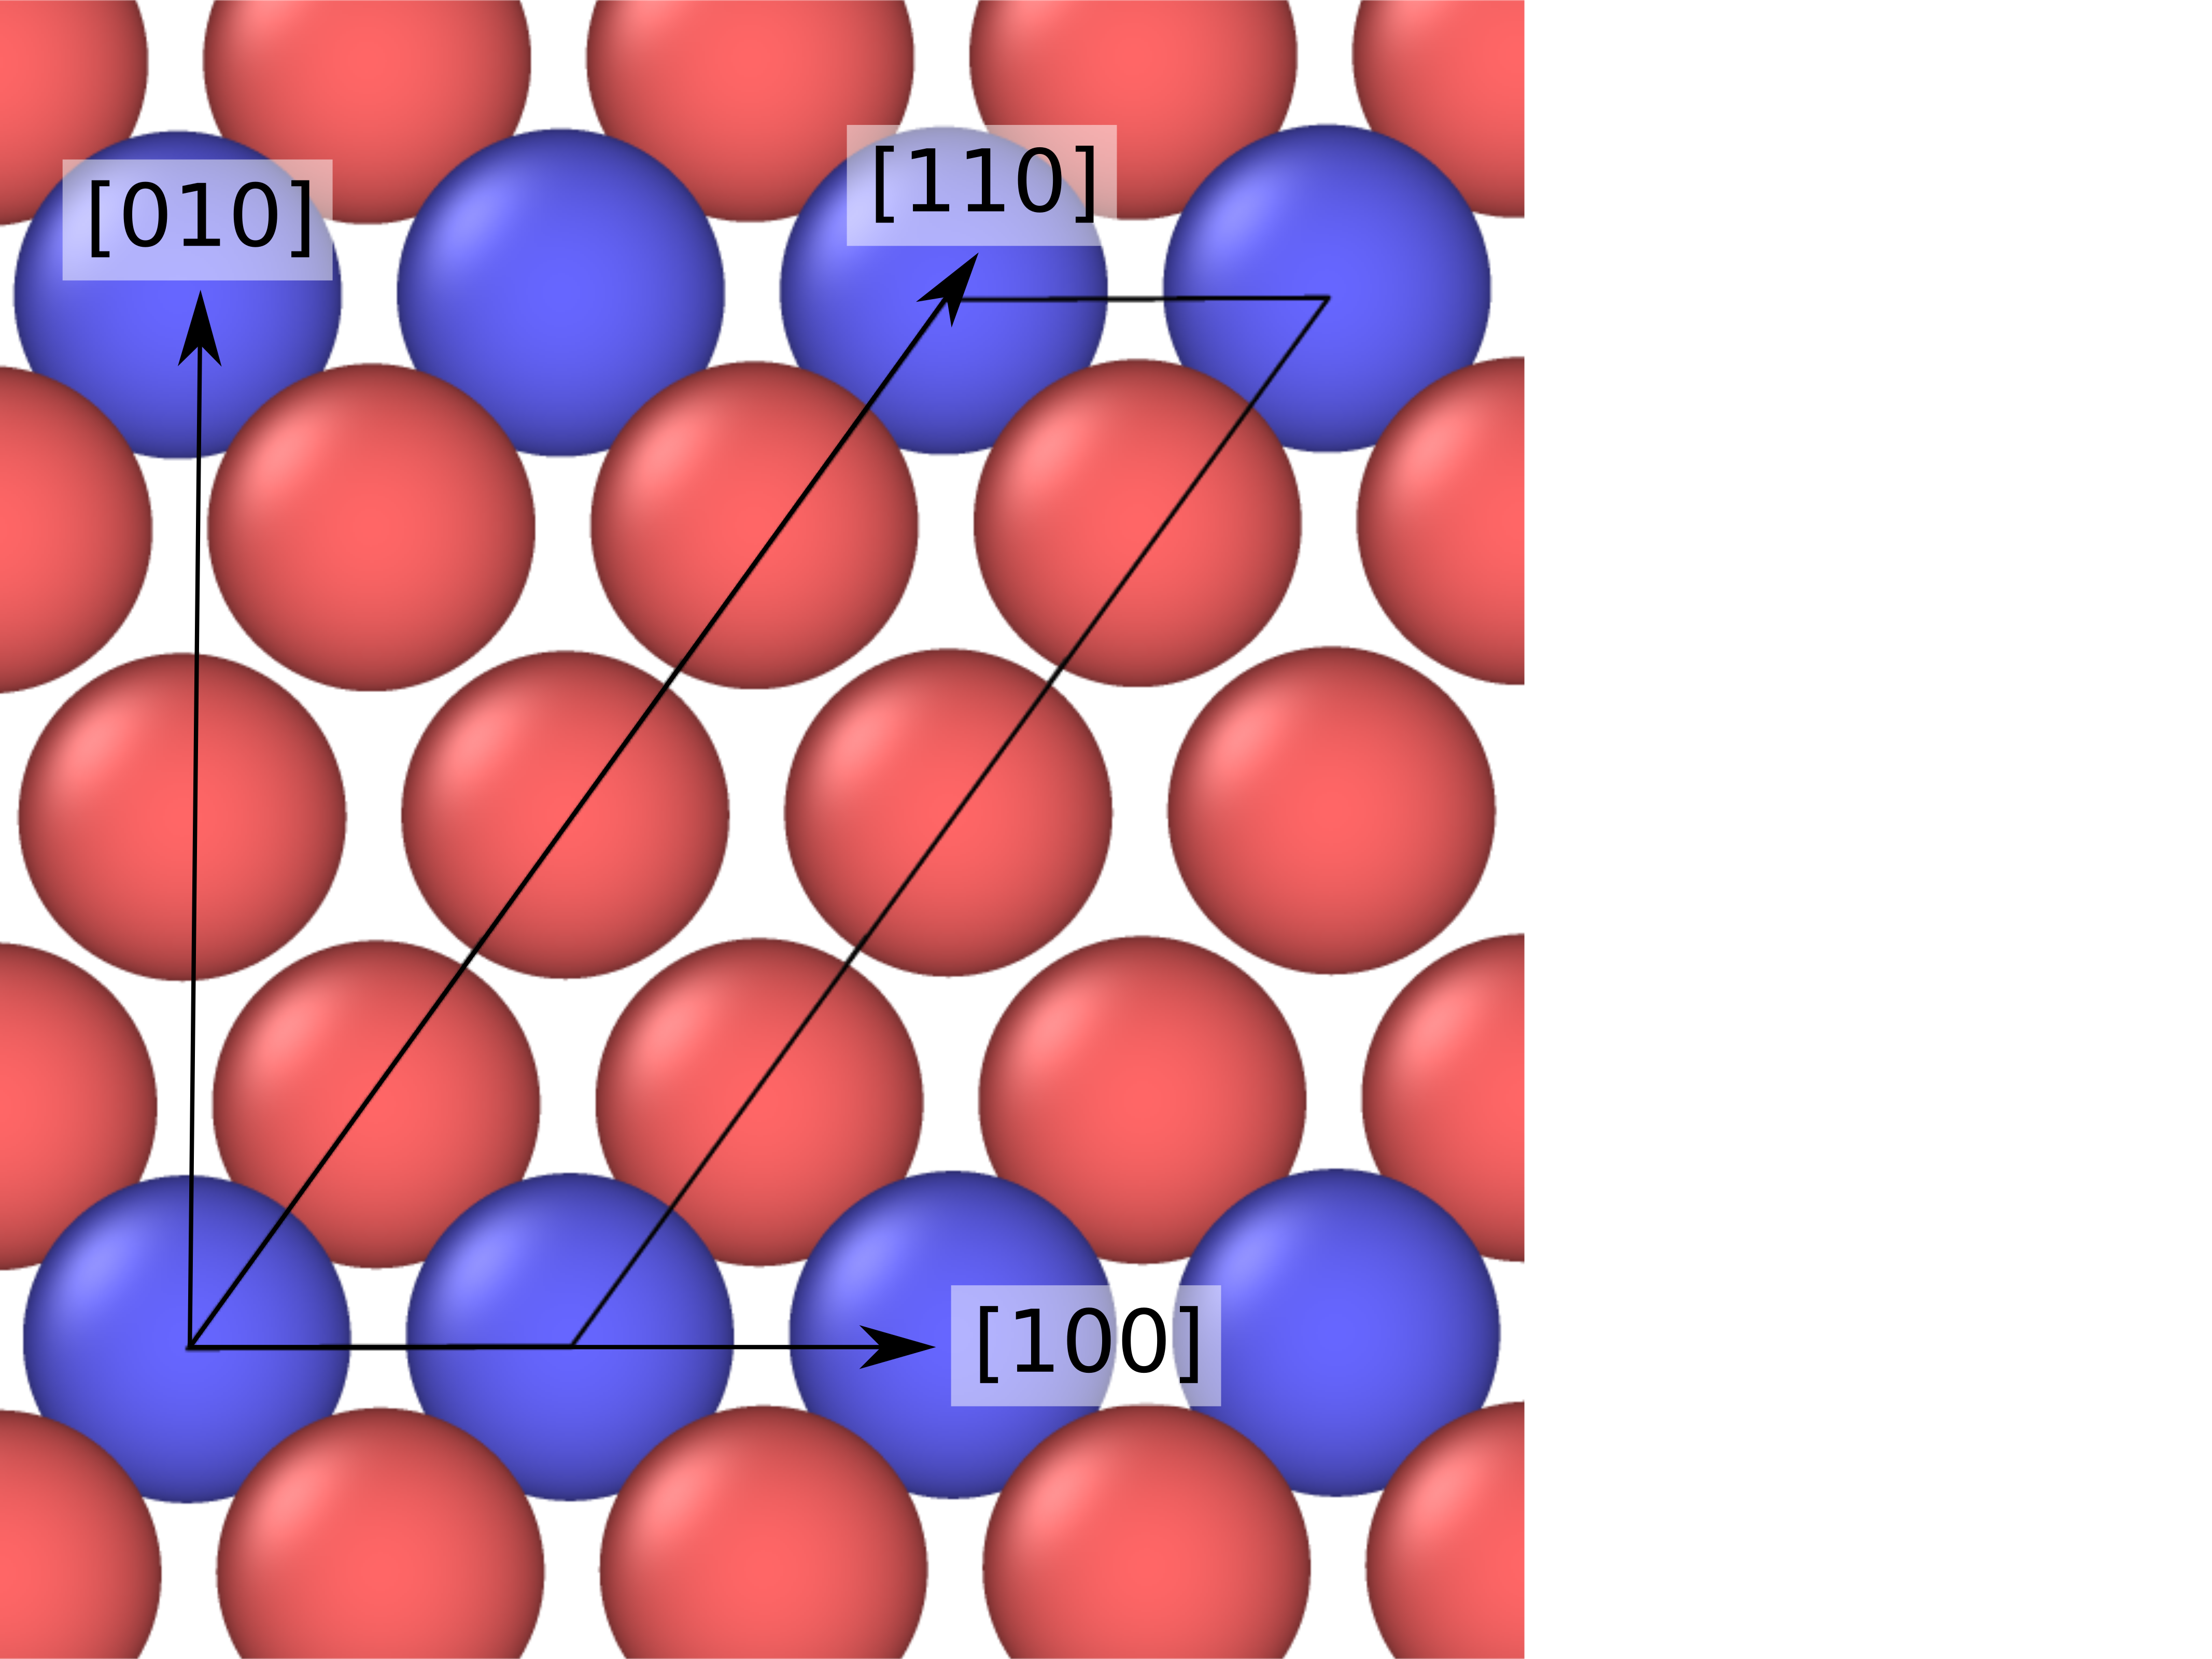
\includegraphics[width=0.32\textwidth]{figures/GSF_ThetaDP111_AtomicView.png}
 }}%
\subfloat[]{{
 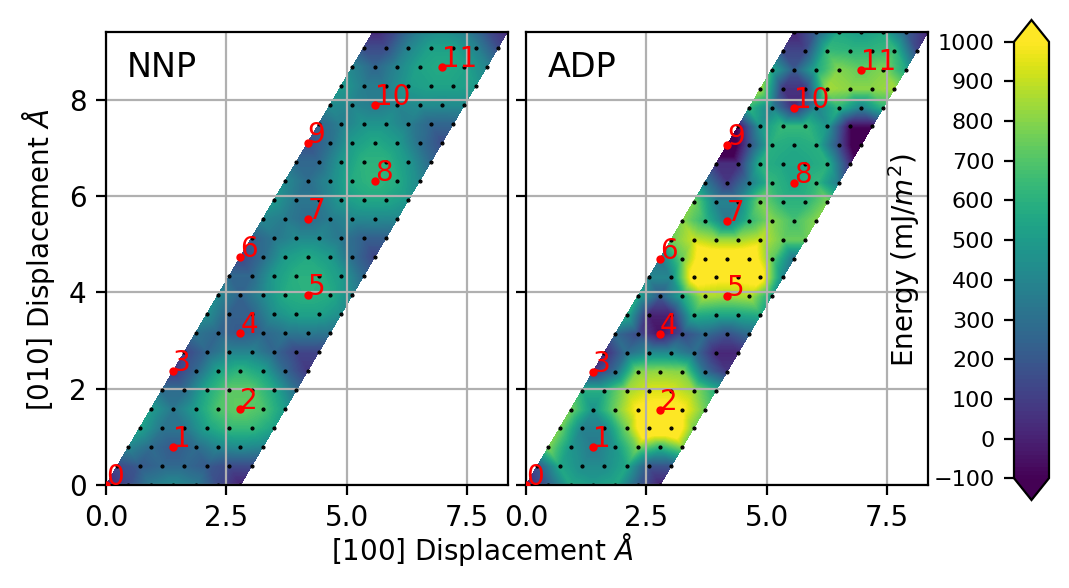
\includegraphics[width=0.68\textwidth]{figures/GSF_ThetaDP111_surf.png}
 }}%
\\
\subfloat[]{{
 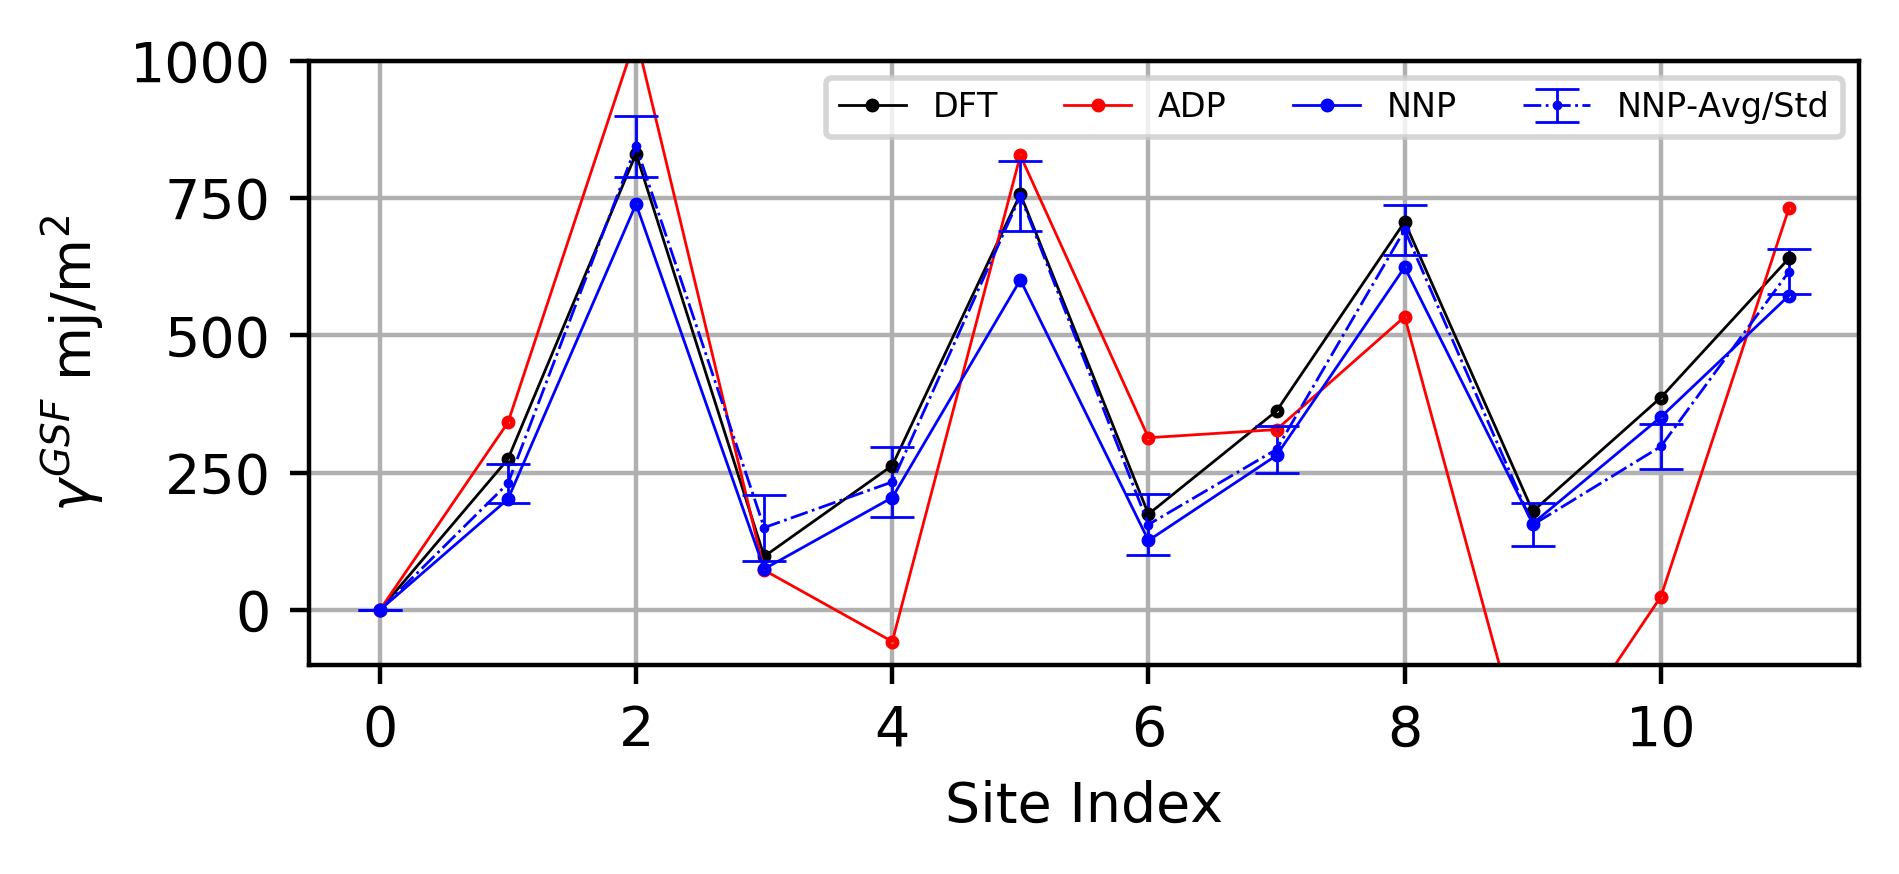
\includegraphics[width=1.00\textwidth]{figures/NOTINOQMD_00002-GSF_111.png}
 }}%
\caption{(a) GSFE and (b) atomic coordinates for the $\theta''$ (111) surface. 
In (b), each black dot represents a point of calculation for NNP and ADP, while the red numbered dots are sites that were computed with DFT.
(c) Site index vs. GSF energy for DFT, NNP, and ADP.
While bulk $\theta''$ was included
in training set, the GSF calculations were not.}
\label{fig:GSF_ThetaDP_111}
\end{figure}

\begin{figure}[H]%
\centering%
\subfloat[]{{
 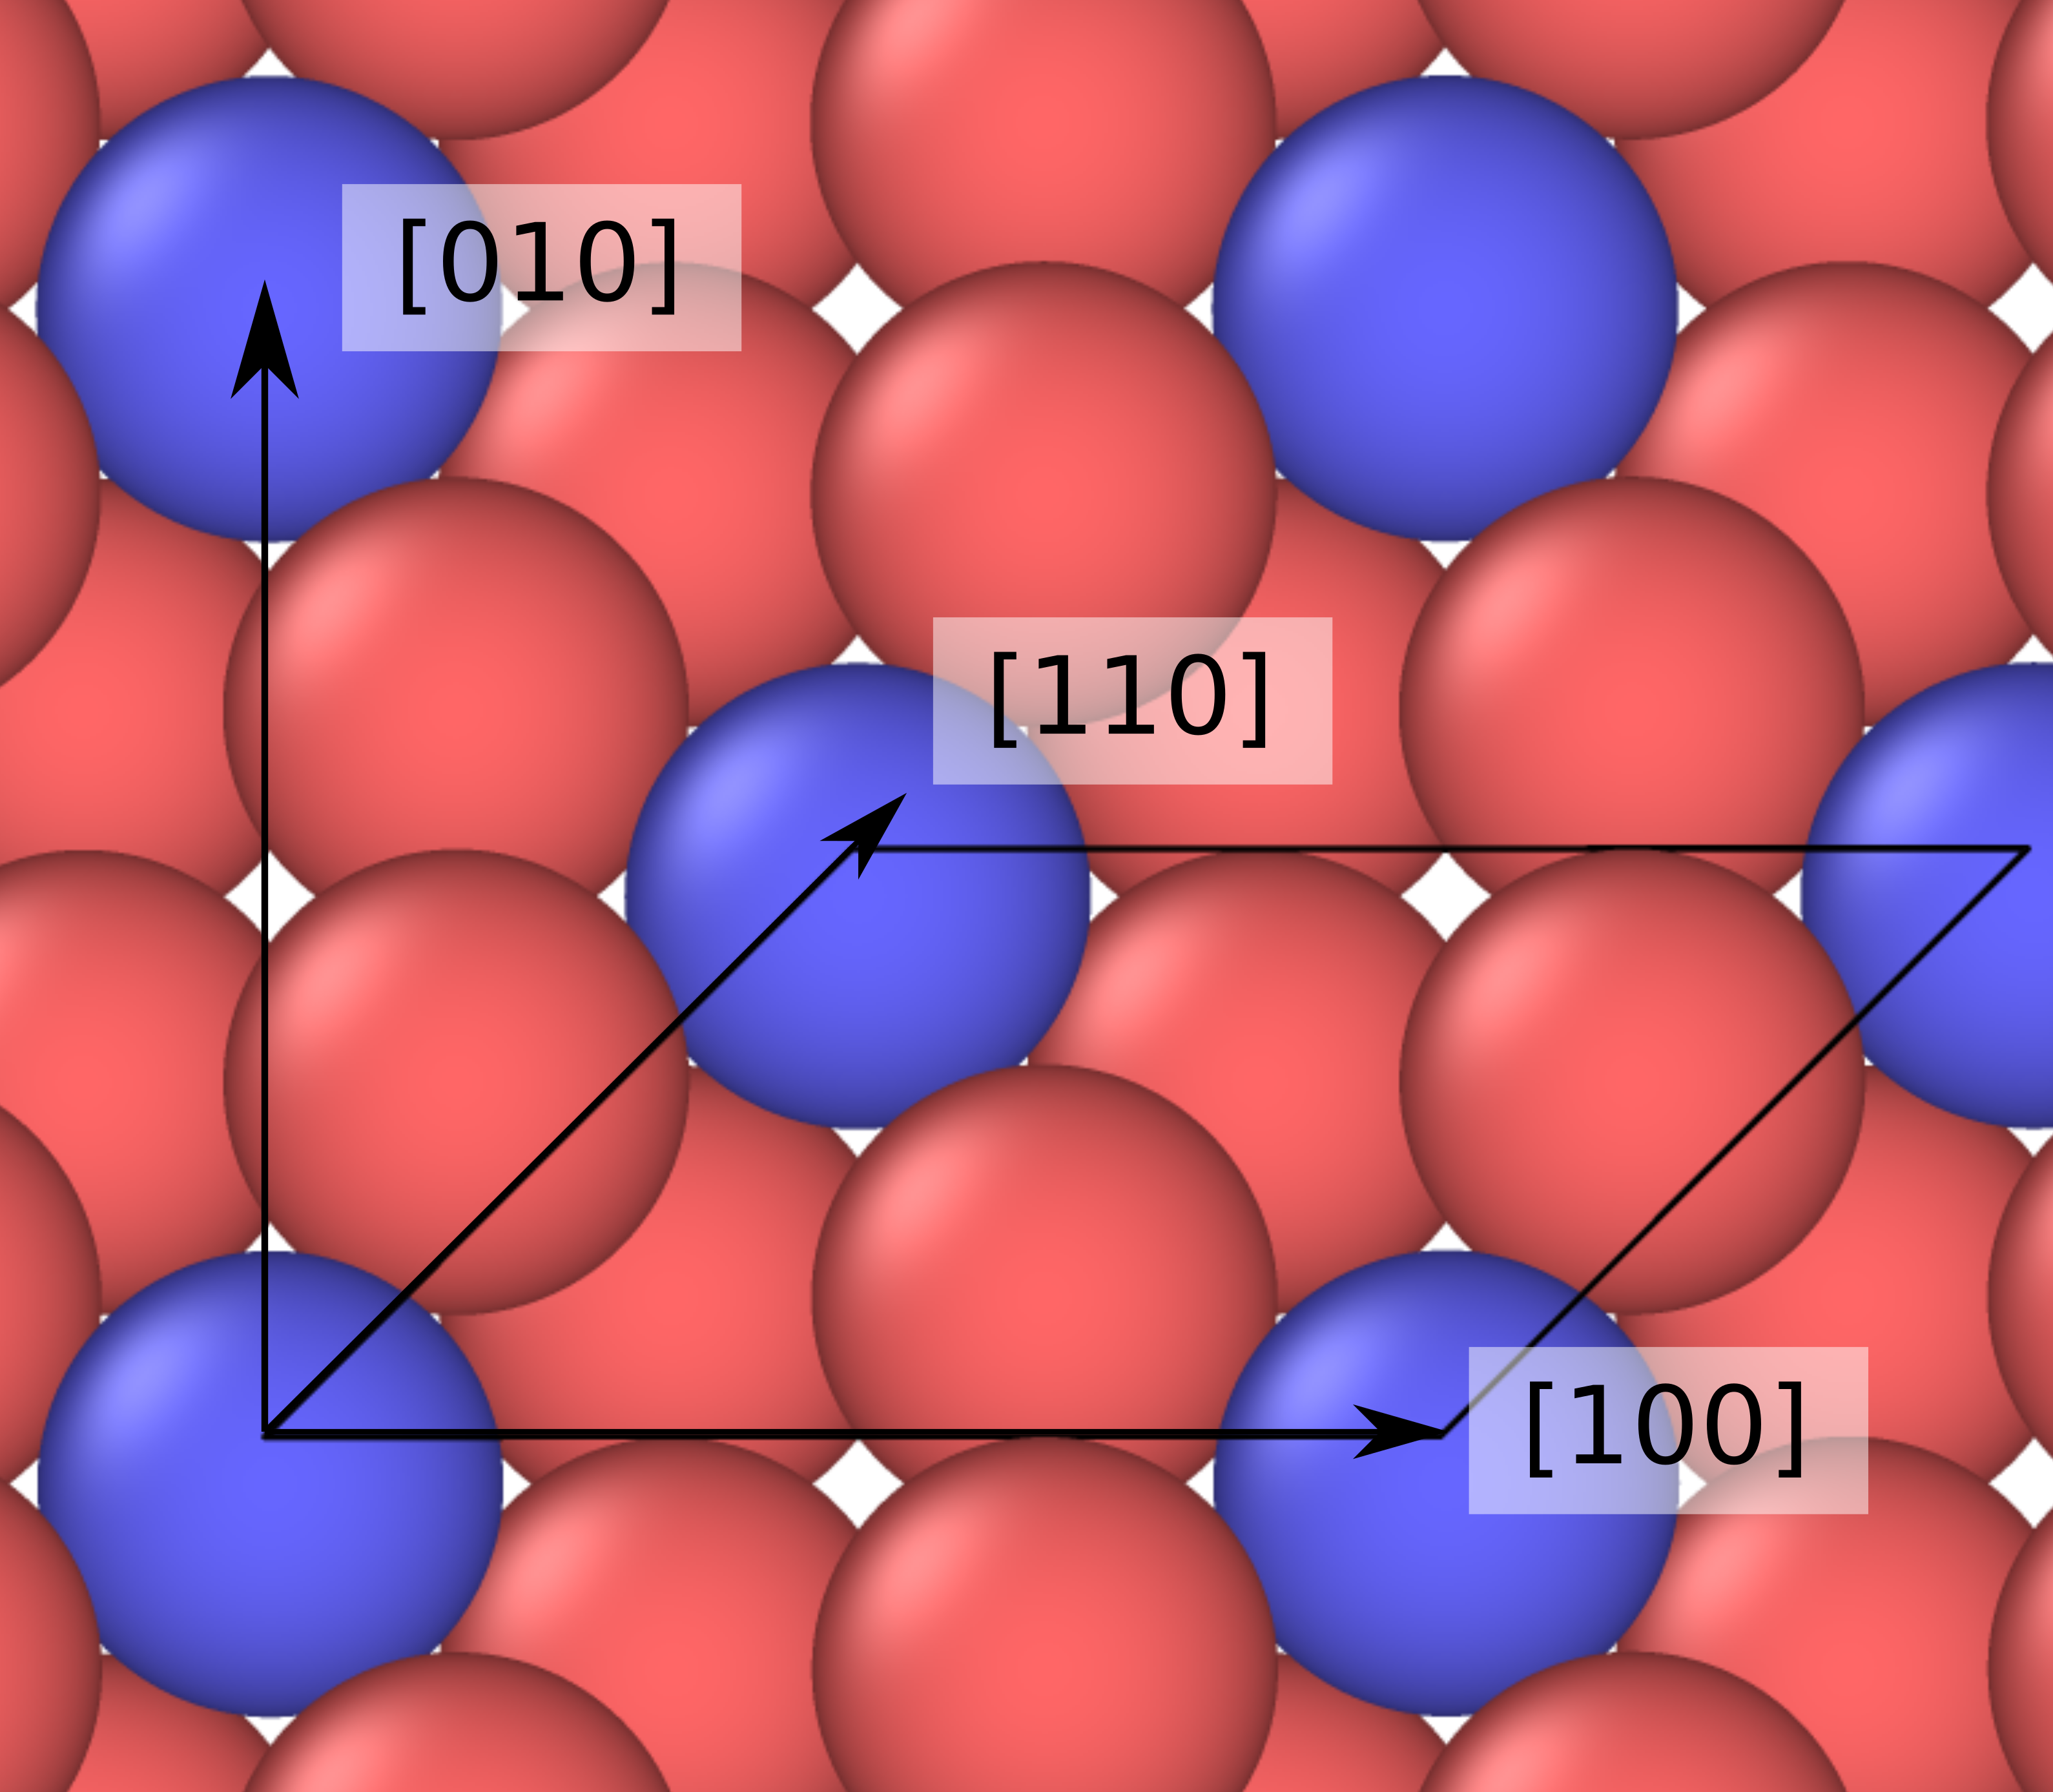
\includegraphics[width=0.40\textwidth]{figures/GSF_Theta0m11_AtomicView.png}
 }}%
\subfloat[]{{
 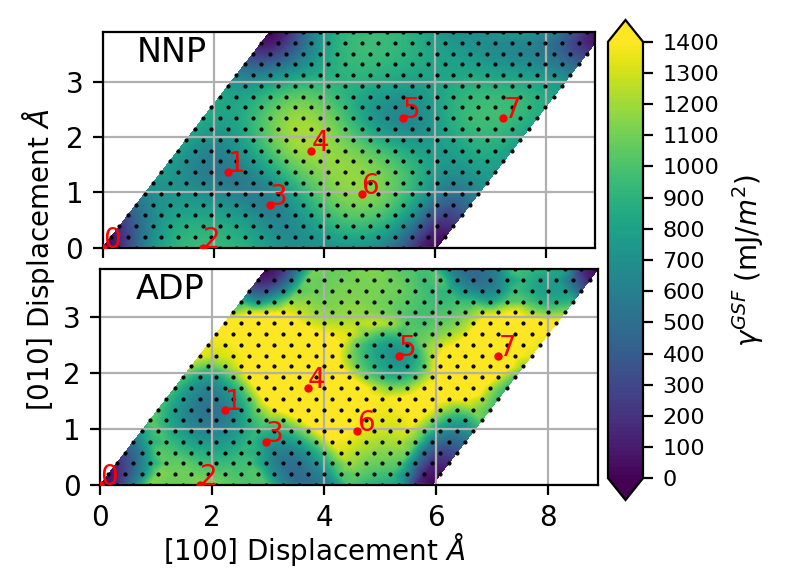
\includegraphics[width=0.60\textwidth]{figures/GSF_Theta0m11_surf.png}
 }}%
\\
\subfloat[]{{
 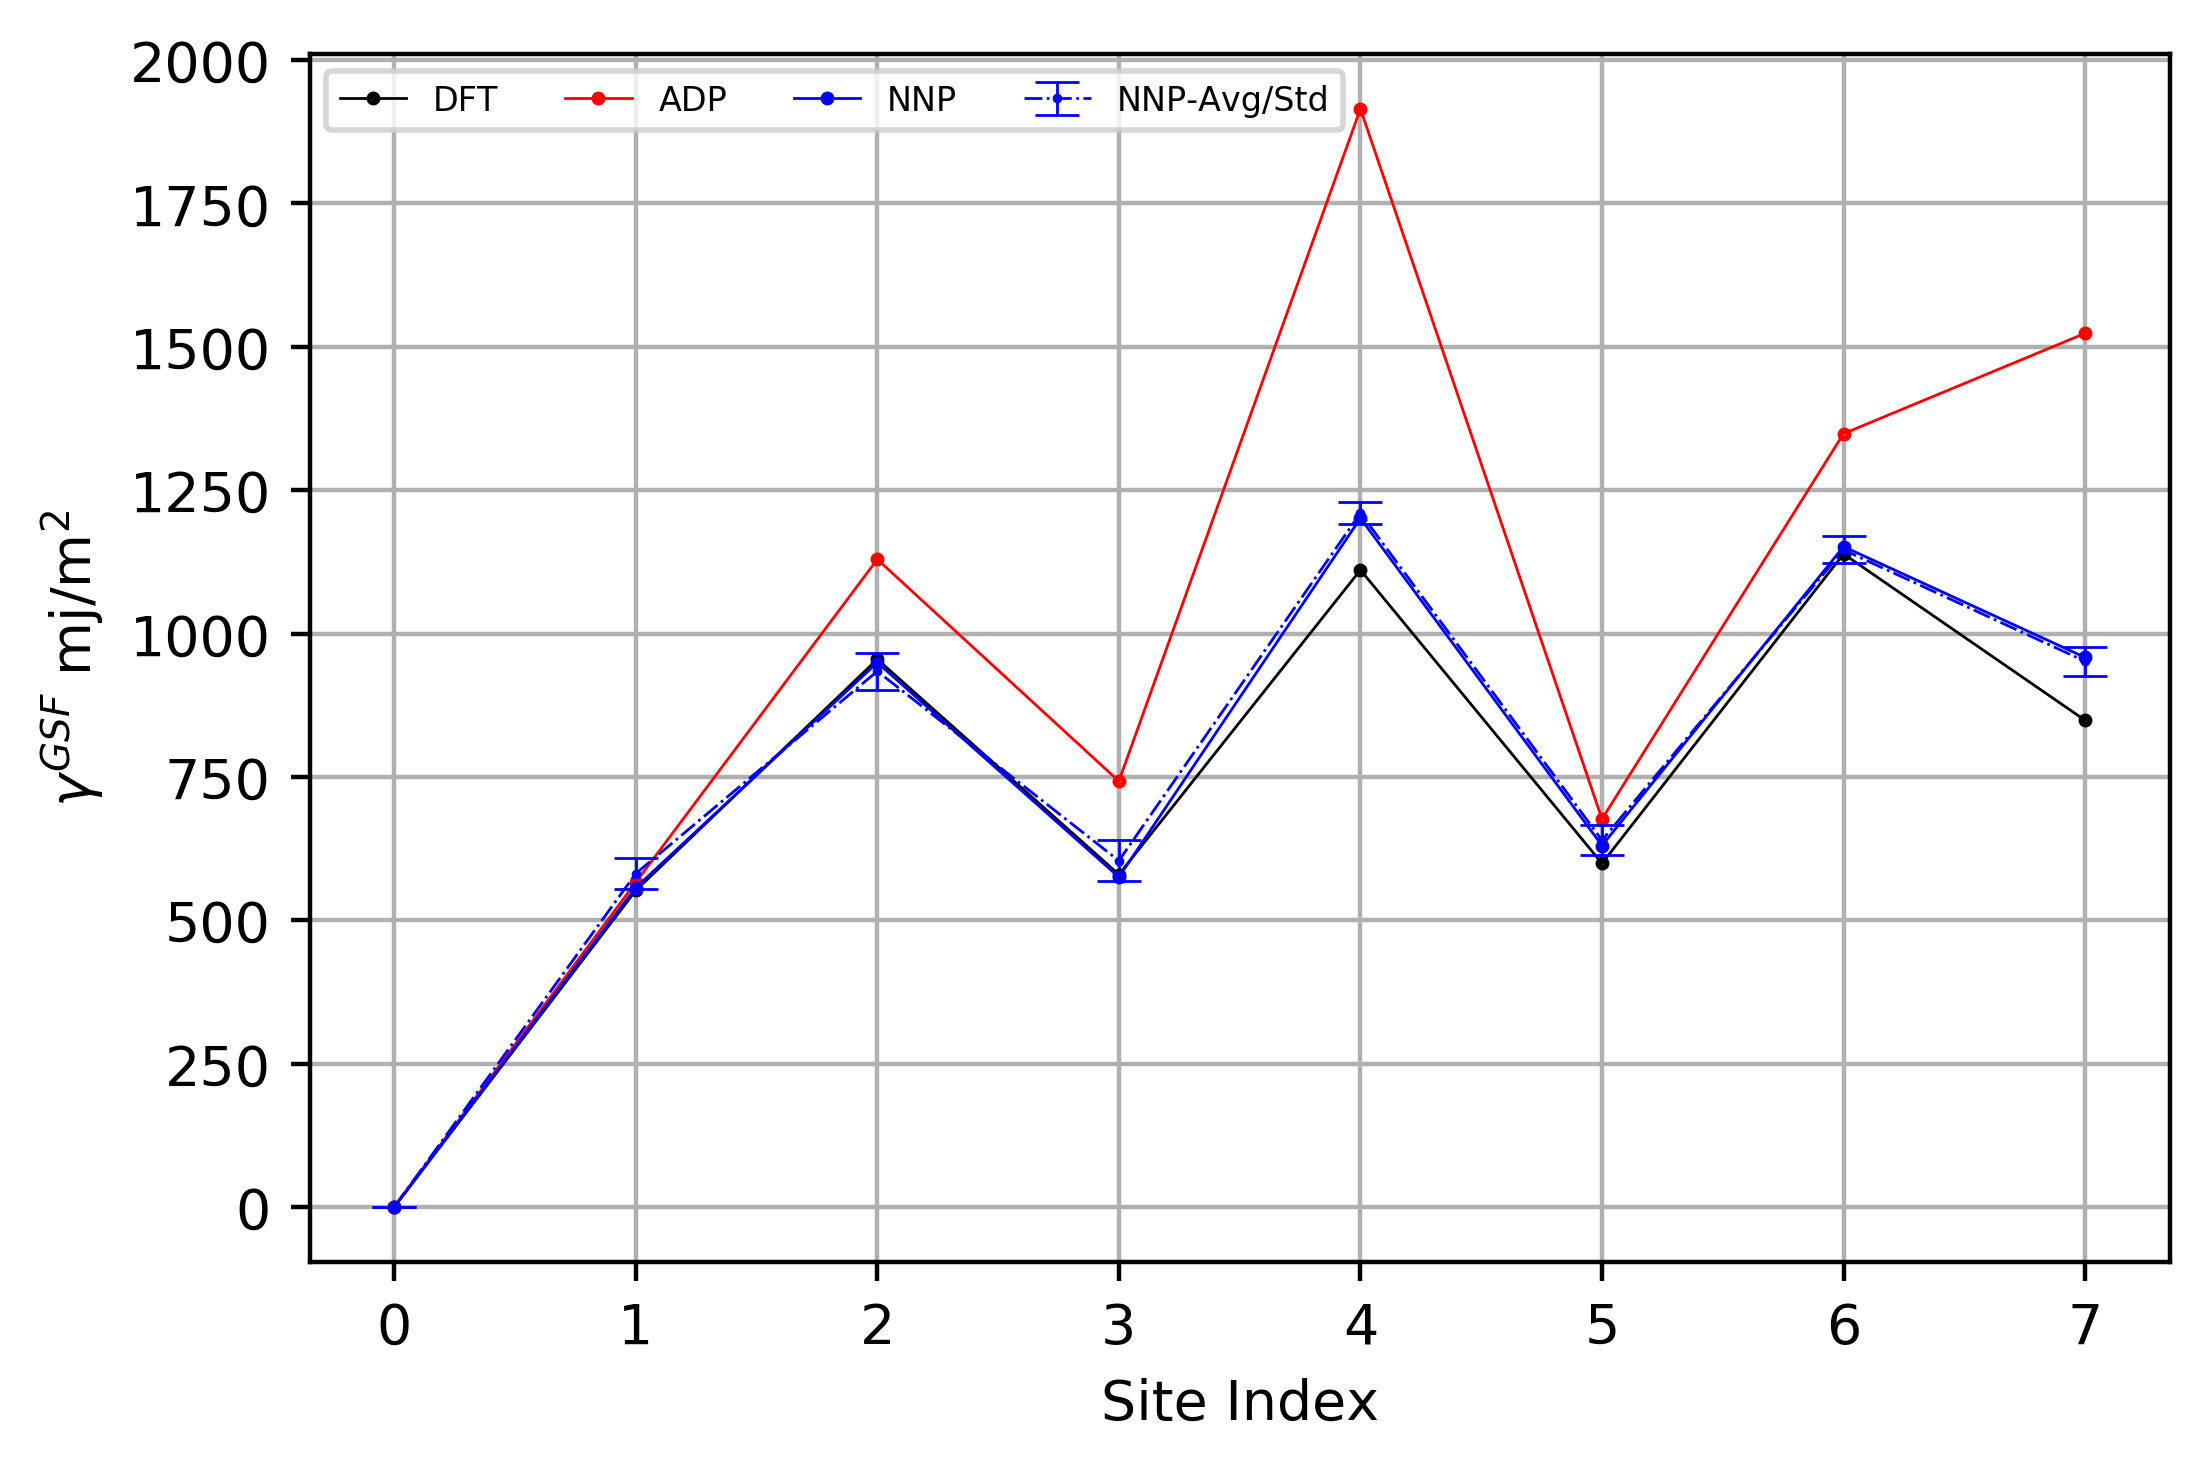
\includegraphics[width=1.00\textwidth]{figures/NOTINOQMD_00001-GSF_0m11.png}
 }}%
\caption{(a) GSFE and (b) atomic coordinates for the $\theta$ (0$\overline{1}$1) surface. 
In (b), each black dot represents a point of calculation for NNP and ADP, while the red numbered dots are sites that were computed with DFT.
(c) Site index vs. GSF energy for DFT, NNP, and ADP.
Indexed sites are included in the training set.}
\label{fig:GSF_Theta_0m11}
\end{figure}

\subsection{Antisites and Vacancies}
Antisite and vacancy formation energies were calculated for every OQMD structure in the following manner.
Firstly, the structure was allowed to be completely relaxed.
If the structure maintained the same symmetry group after full cell and atomic relaxation, we analyzed it for unique atomic sites using pymatgen.
Then the cell was duplicated, such as to generate cells with a minimum of 108 atoms to minimize defect-defect interactions.
For each of the unique sites identified, we then swapped it with the different atom, e.g., Al $\rightarrow$ Cu or Cu $\rightarrow$ Al, else we deleted the site to generate a vacancy and stored the antisite structure.
The energies of all antisite structures were calculated without relaxation.
This equation gave the antisite formation energies $\Delta E^{antisite}_f$:
\begin{equation}
\Delta E^{antisite}_f = E^{antisite} - E^{pristine} - \sum\Delta n_i E^{ref}_i
\end{equation}
Where $E^{antisite}$, $E^{pristine}$ are the total energies of the antisite, and pristine structure, $n_i$ is the 
number and sign of the swapped atoms, and $E^{ref}_i$ is the reference energy for compound $i$, as stated in 
equations \ref{eqn:formRef_Al} and \ref{eqn:formRef_Cu}.

Figure \ref{fig:antisite_plot} shows the antisite results.
Error bars rarely exceed 0.1eV and are almost always centered around the correct DFT value.
ADP also performs reasonably but has substantially more errors, with many samples deviating more than 1eV from DFT.
These results demonstrate that NNPs make accurate predictions of defects that are not in their training set. 

\begin{figure}[H]%
\centering%
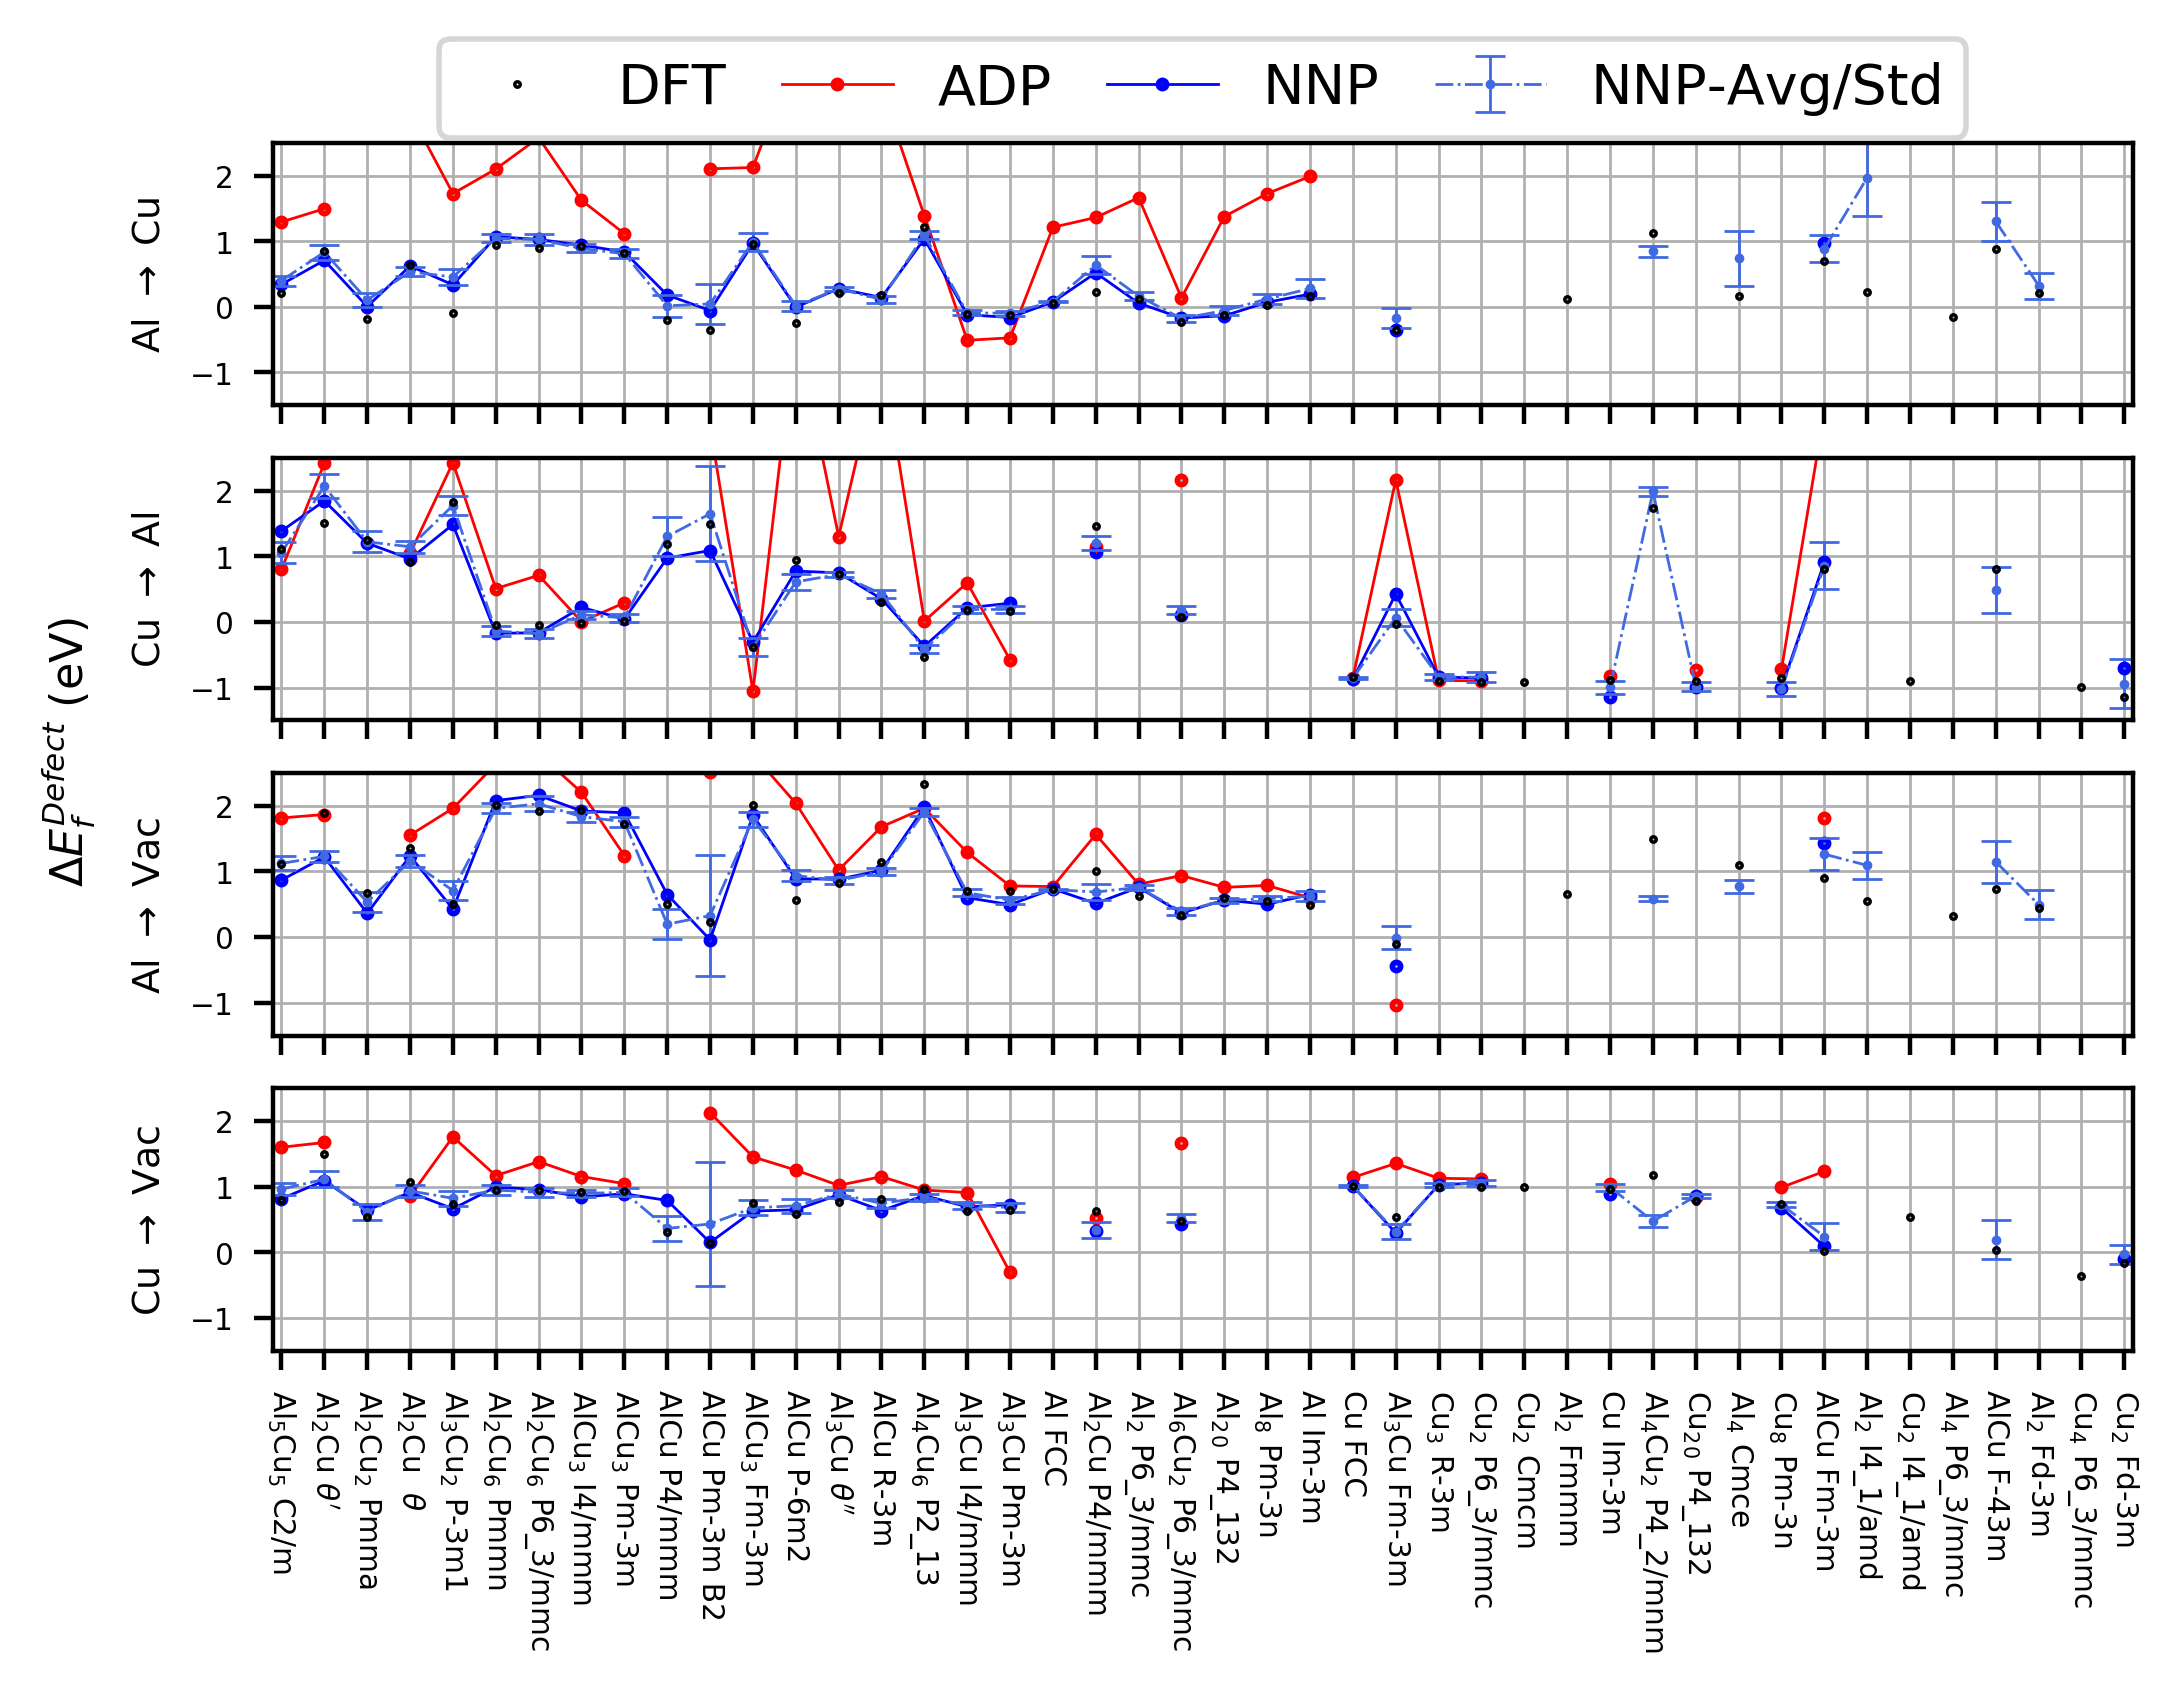
\includegraphics[width=1\textwidth,center]{figures/antisite_vacancies.png}%
\caption{DFT antisite formation energy vs. ADP/NNP antisite formation energy.
These structures were not included in the training set.}%
\label{fig:antisite_plot}
\end{figure}

\textcolor{red}{\subsection{Albert Section}}

\section{Conclusion}
In this work, we have developed an NNP, comprehensively compared it to the most currently-used interatomic potential, ADP, and found ours to be a significant step forward in the state-of-the-art.
ADP is physically-derived and has far fewer parameters than an NNP, so it performs nearly equal to or (as in the case of C44 in Aluminum) better than NNP, on simple properties in simple structures.
However, our NNP has a massive advantage when considering a broad range of structures in complex environments.
For example, the NNP reproduces the formation energy of all stable compounds within the OQMD (and most of the unstable ones as well) down to a few meV, which is utterly impossible for the ADP potential.
For binary solutes included in the training set, the NNP rarely predicts energies with an error beyond 20meV, while ADP makes errors of several hundred meV for binaries.
NNP shows decent accuracy even for solute clusters that are not in the training set, such as the ternary and quaternary clusters.
The NNP shows many advantages even on the essential $\theta''$, $\theta'$, $\theta$ family of precipitates.
The GSFE of $\theta''$ for ADP shows massive errors, where it predicts entire regions as stable when they are not; NNP has excellent accuracy for the $\theta''$ GSF, even without explicit training.
\textcolor{red}{One/two sentences about Albert's part}.

The NNP is not perfect; most notably, the C44 of Al has substantial errors, even with careful inclusion of relevant structures.
We also note that the error is biased, so even by generating many NNPs and cherry-picking the best for C44, we could not lower the error below 10\%.
This C44 error seems to be an inherent issue with NNPs, or at least the symmetry functions used in their inputs.
We also found that we could not lower the errors on binary solute energies lower than ~20meV, again despite the careful inclusion of structures in the training set.
Again, our potential usually shows excellent agreement with DFT and is almost always an improvement over ADP.
Importantly, we provide all of the data used in the training, testing, and validation of our potential.
Any new Al-Cu potentials now have a rich, carefully-calculated, and well-curated set of data to serve as a stepping stone and benchmark. 


\newpage
\bibliographystyle{unsrt}  
\bibliography{references}  %%% Remove comment to use the external .bib file (using bibtex).
%%% and comment out the ``thebibliography'' section.

\newpage
\appendix
\section{Supplementary}
\subsection{Equation of State of NNP} \label{sct:eos_data}

\begin{figure}[H]%
\centering%
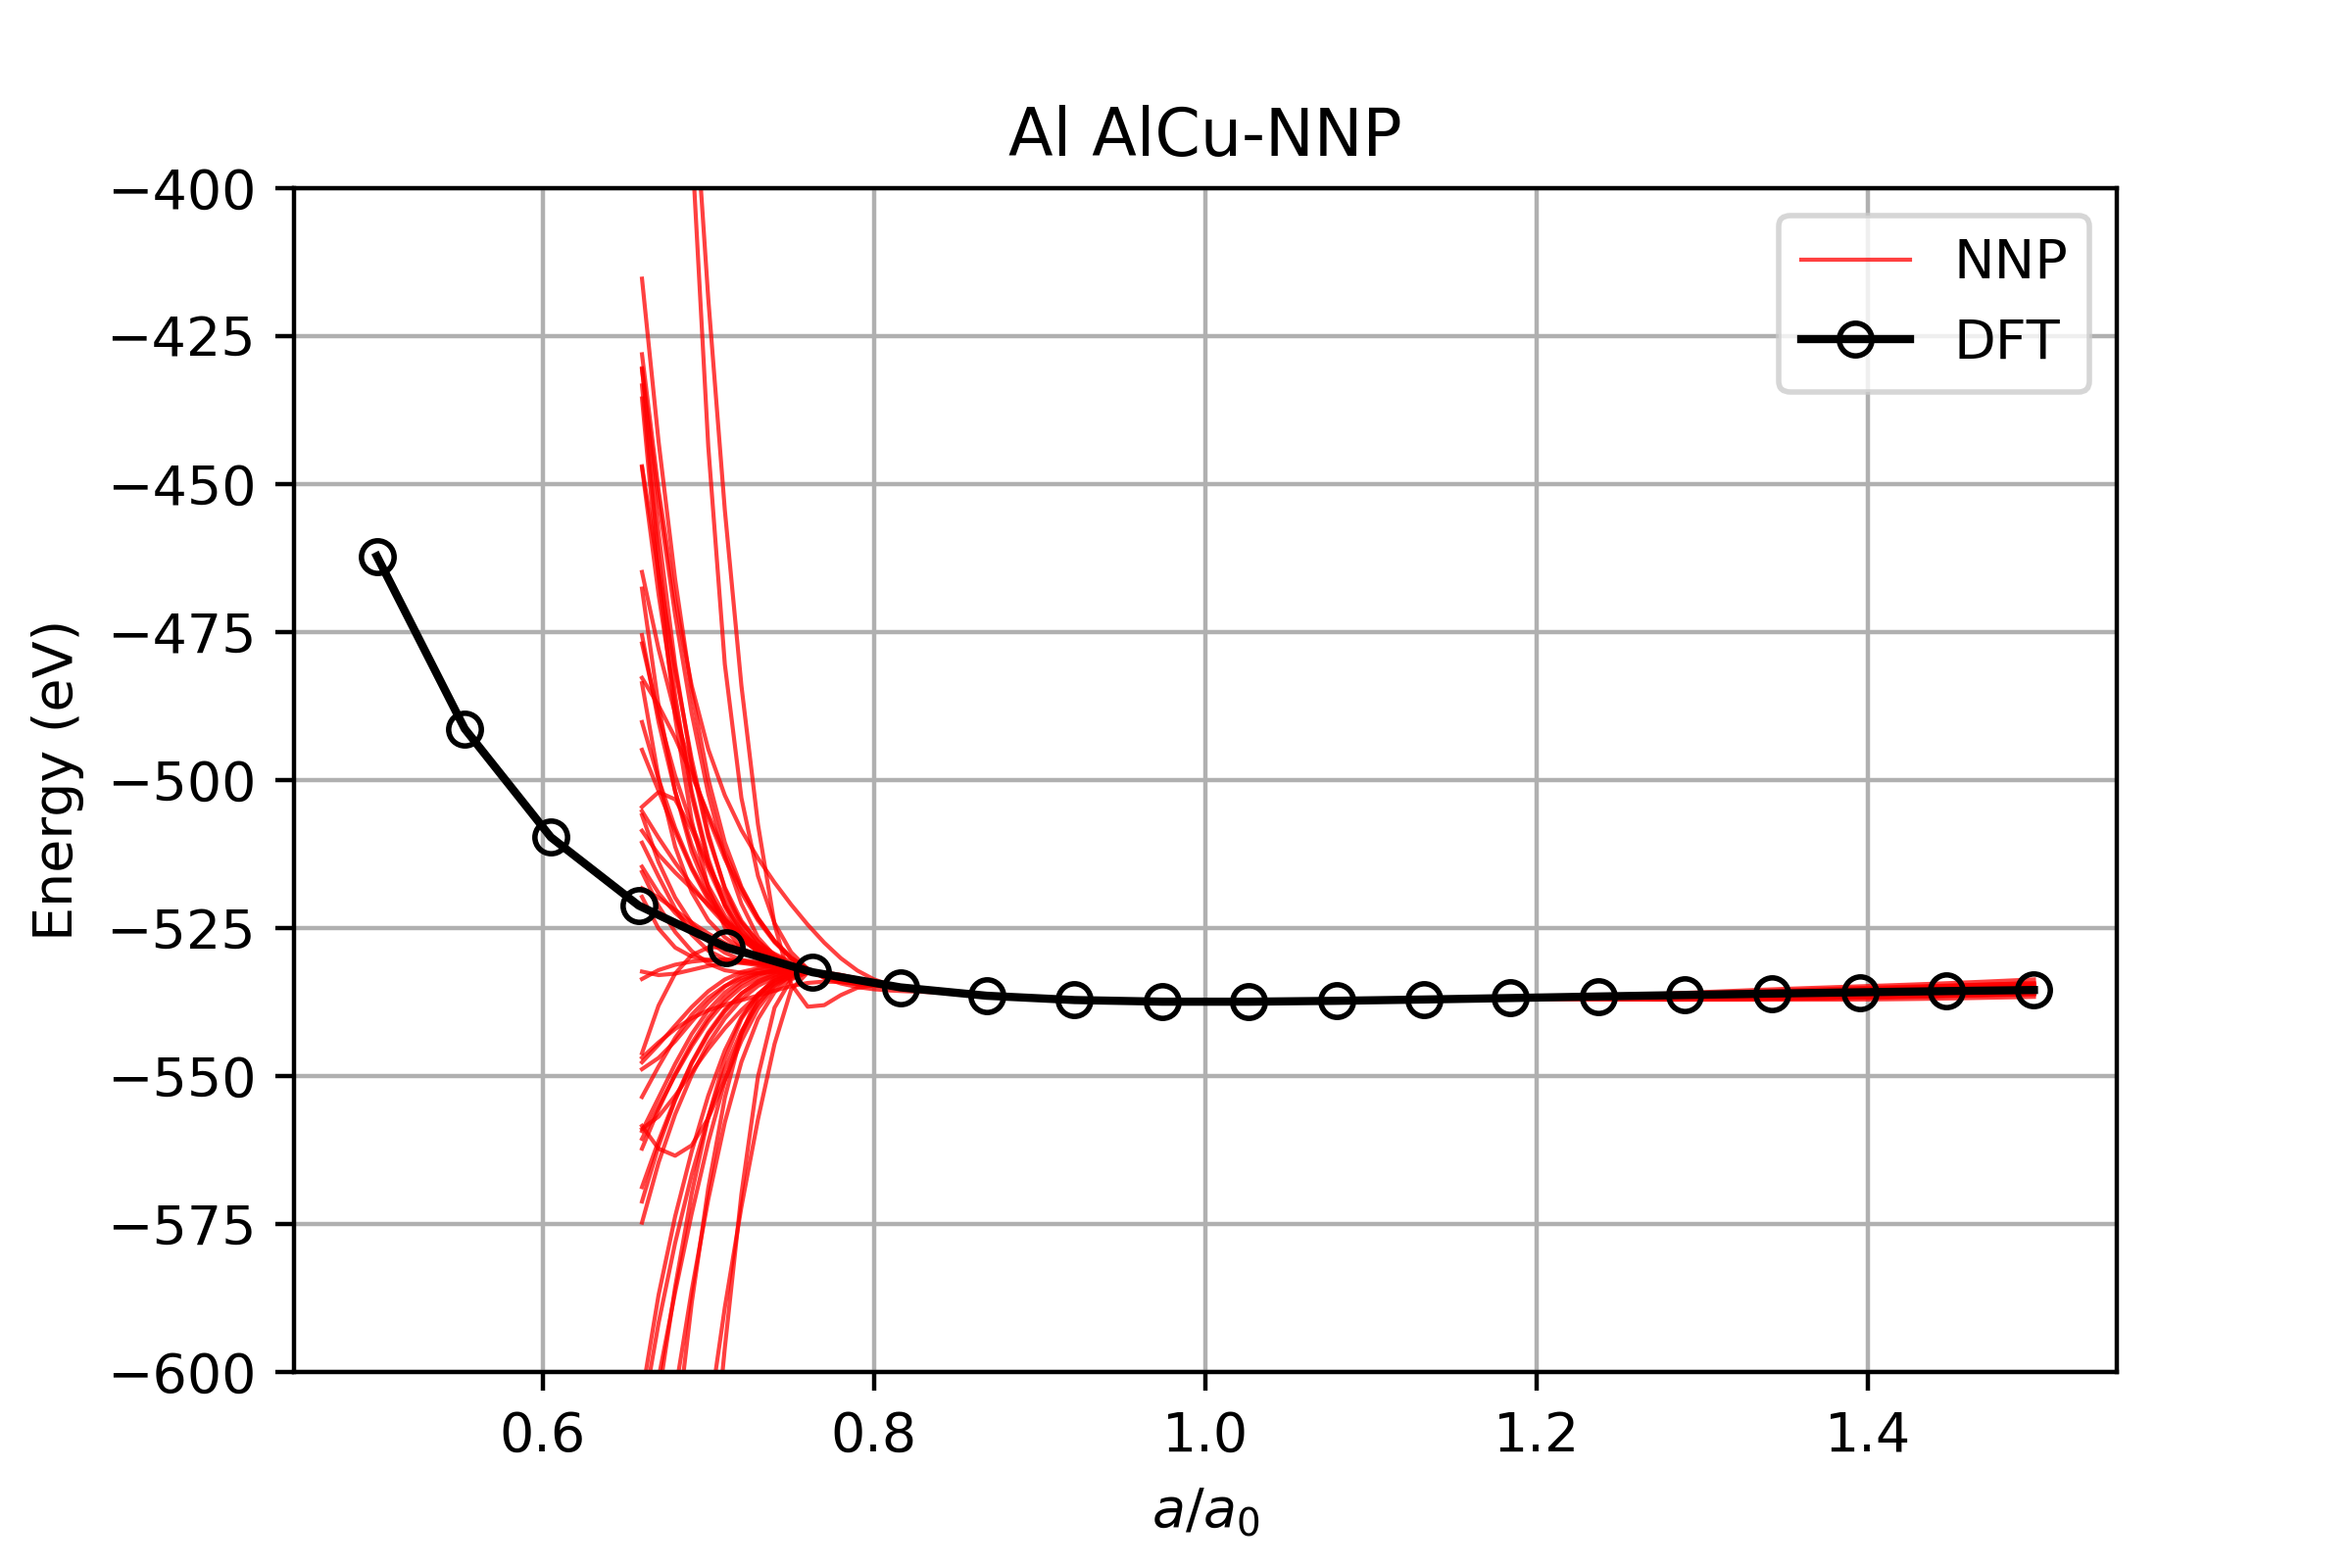
\includegraphics[width=0.7\textwidth,center]{figures/EOS_AlCu-NNP_Al.png}%
\caption{Al equation of state plot}%
\end{figure}

\begin{figure}[H]%
\centering%
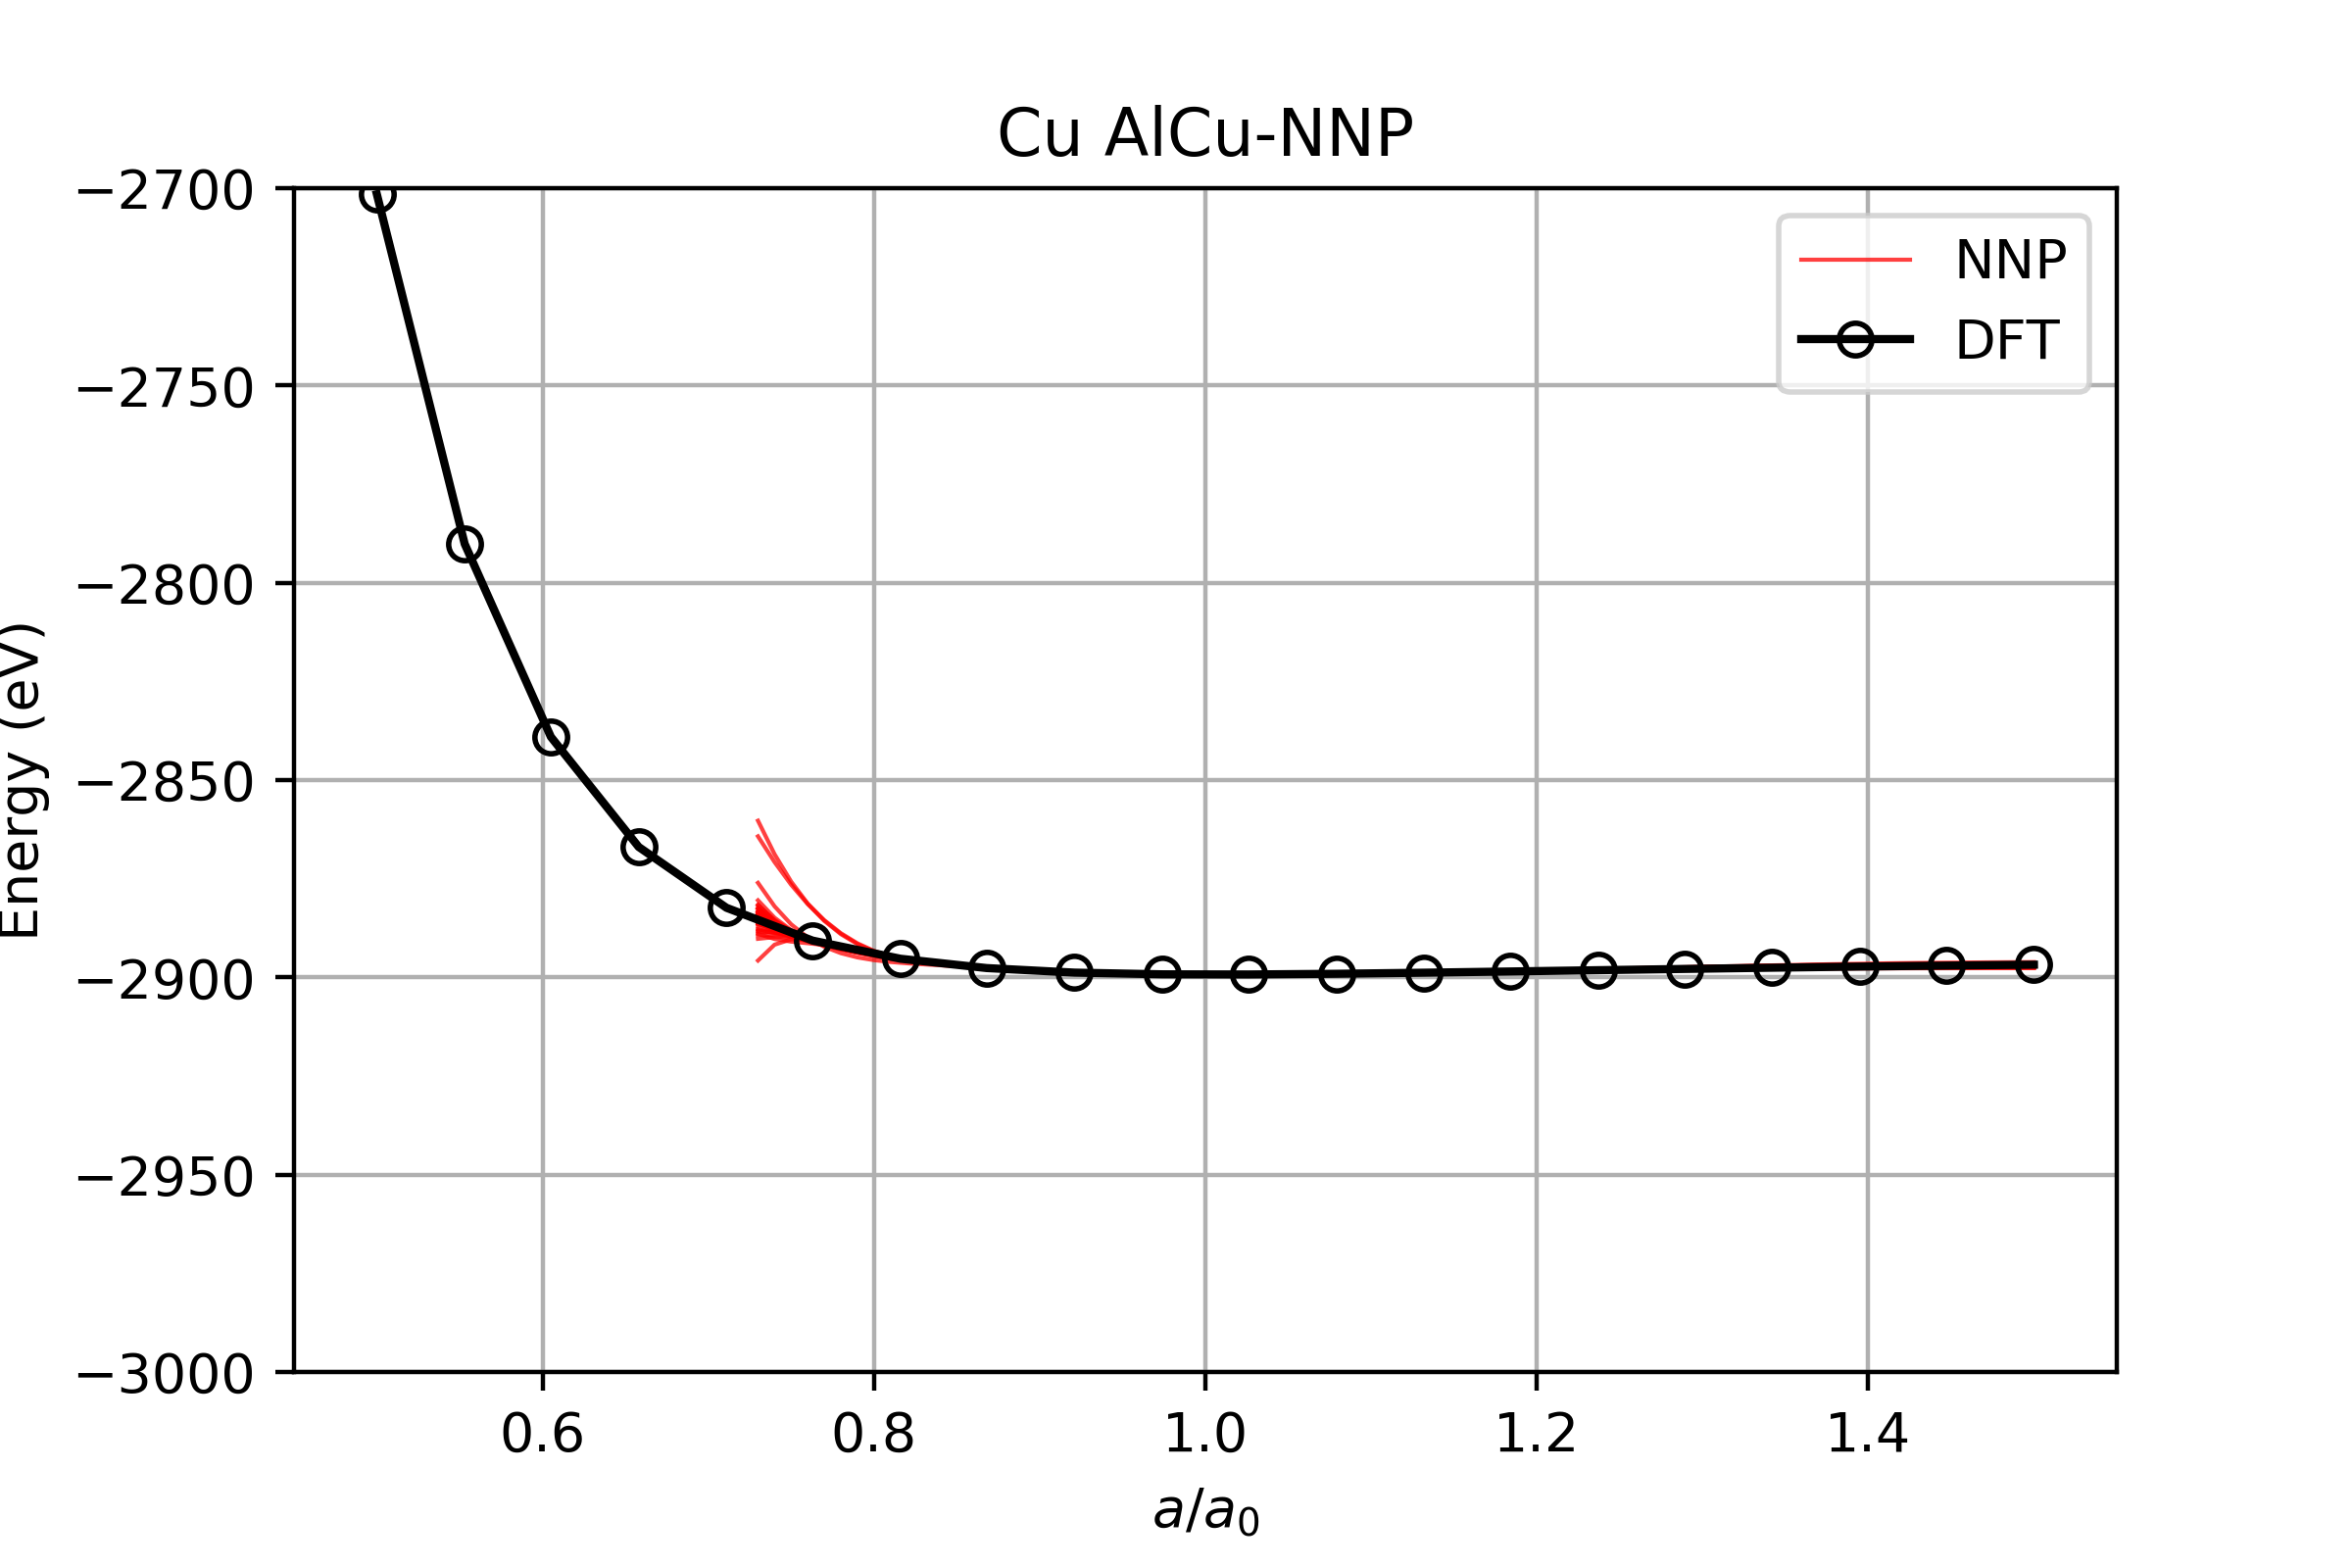
\includegraphics[width=0.7\textwidth,center]{figures/EOS_AlCu-NNP_Cu.png}%
\caption{Cu equation of state plot}%
\end{figure}

\begin{figure}[H]%
\centering%
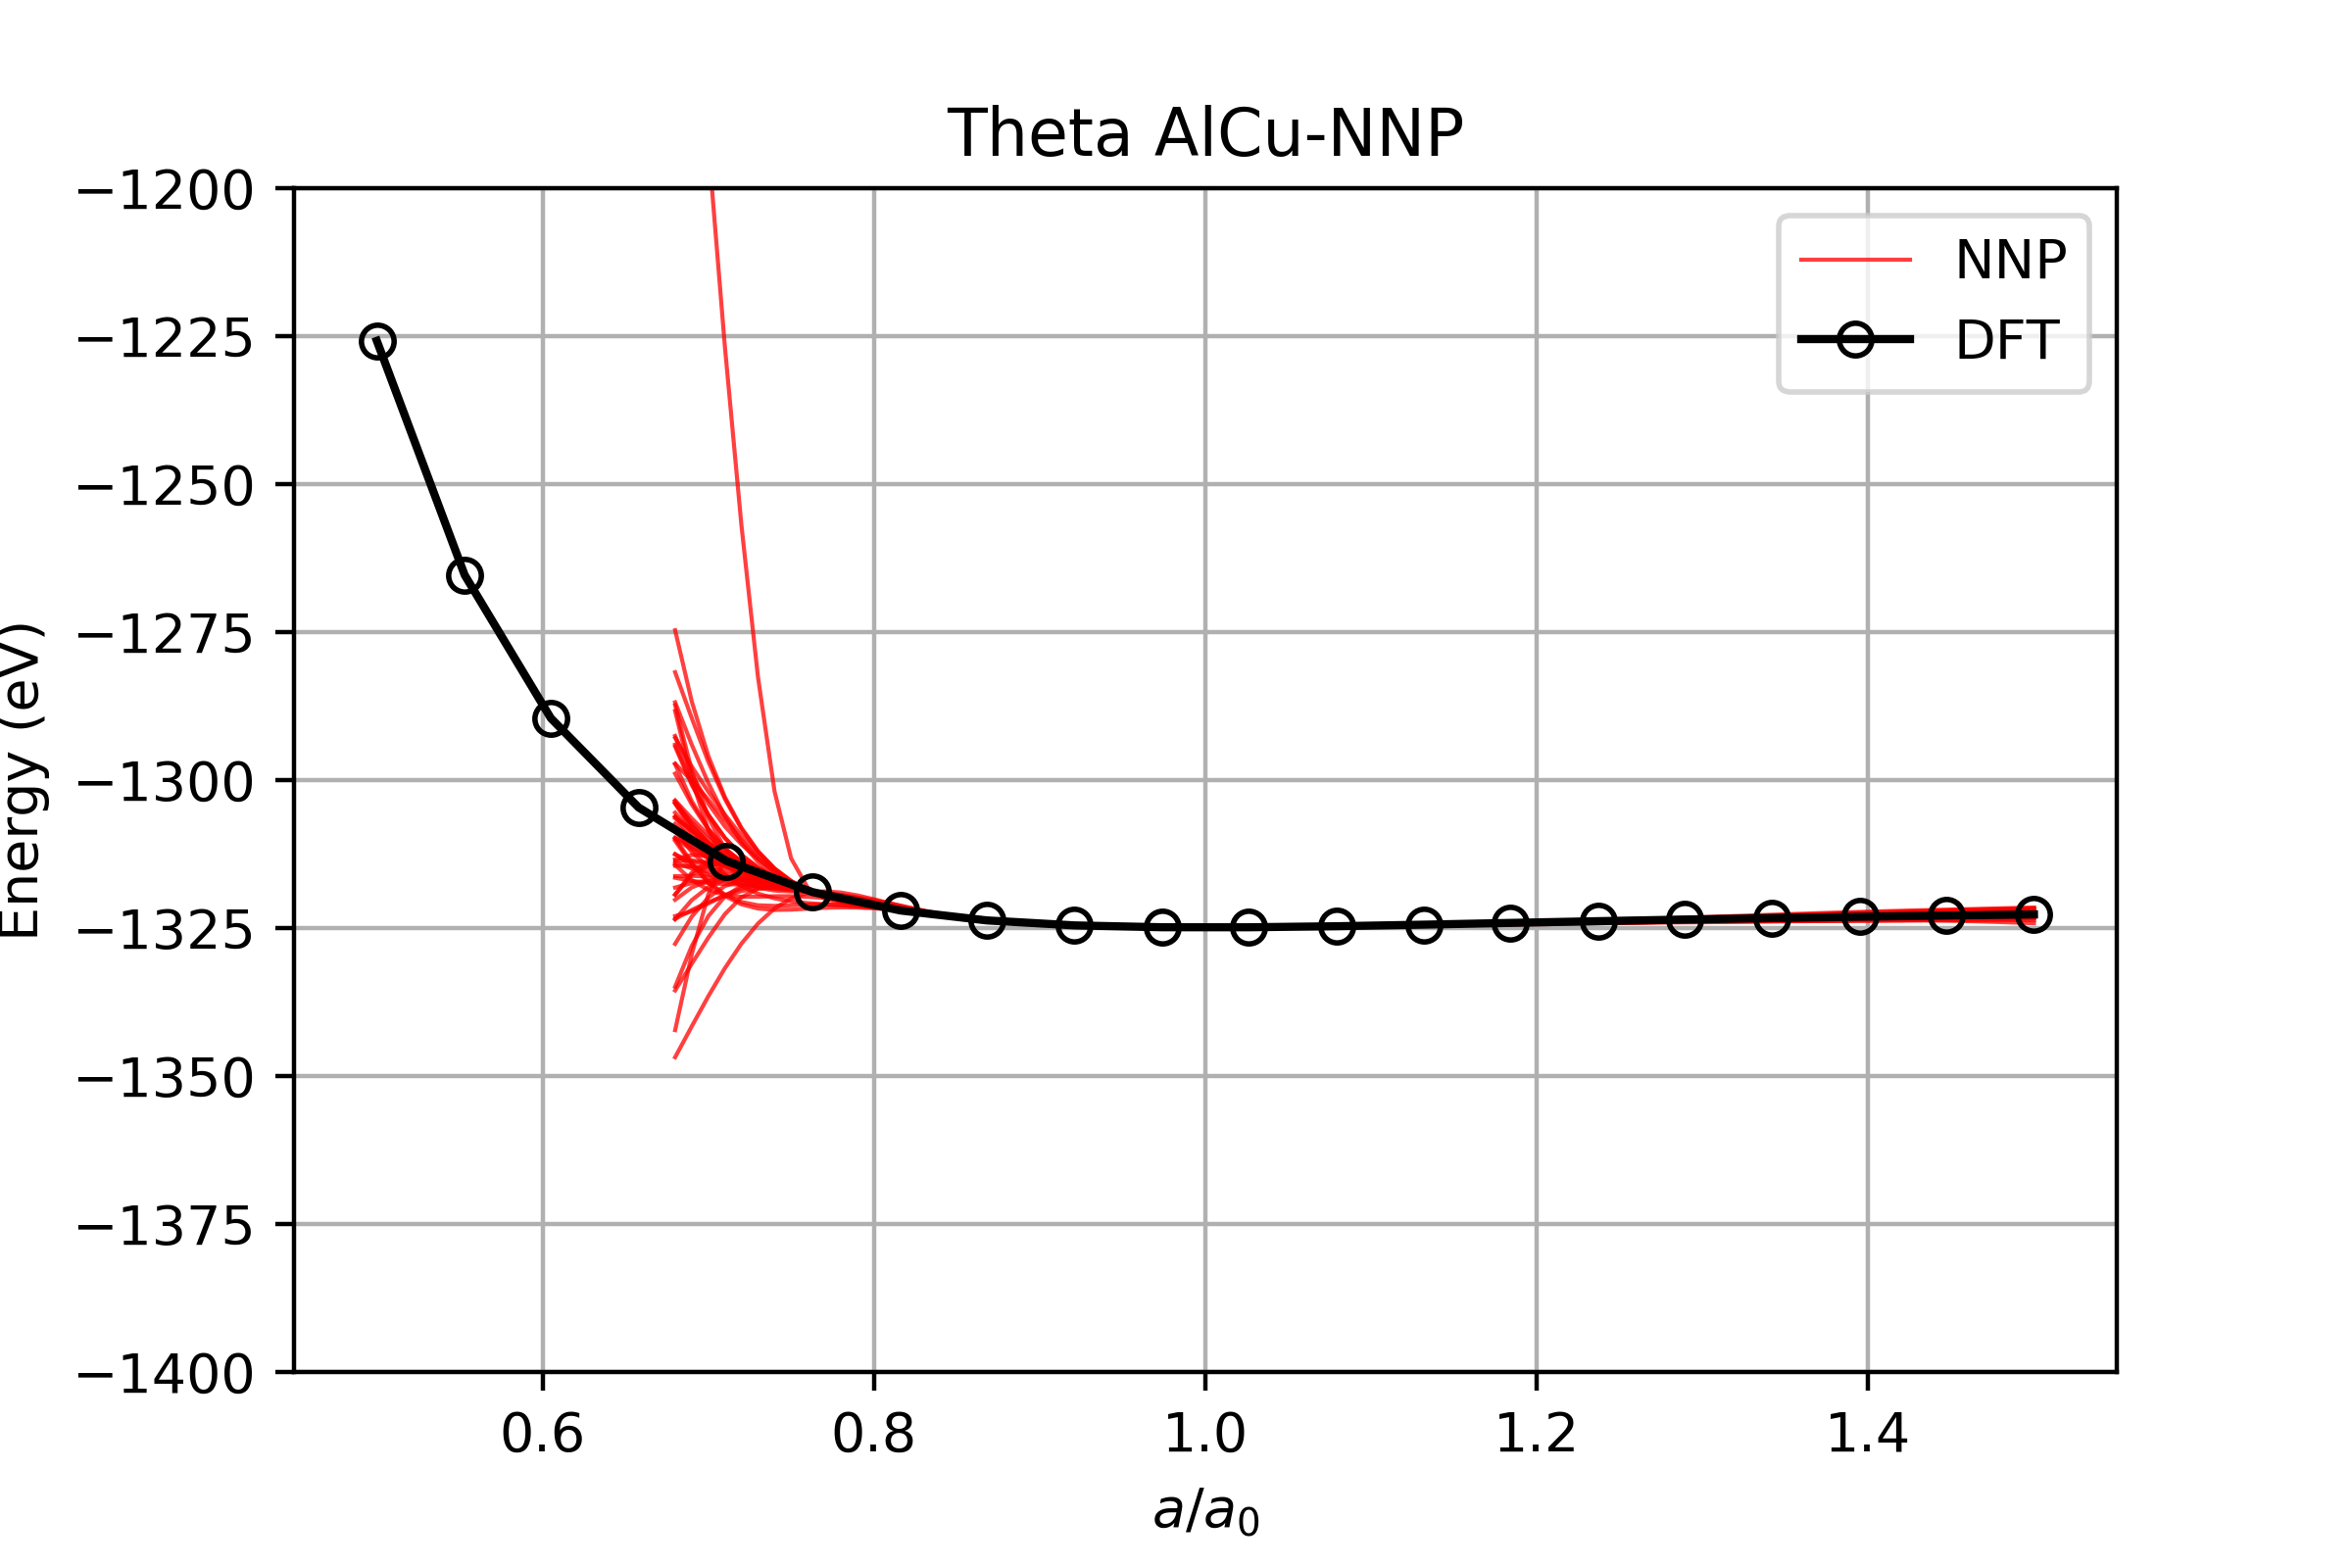
\includegraphics[width=0.7\textwidth,center]{figures/EOS_AlCu-NNP_Theta.png}%
\caption{$\theta$ equation of state plot}%
\end{figure}

\begin{figure}[H]%
\centering%
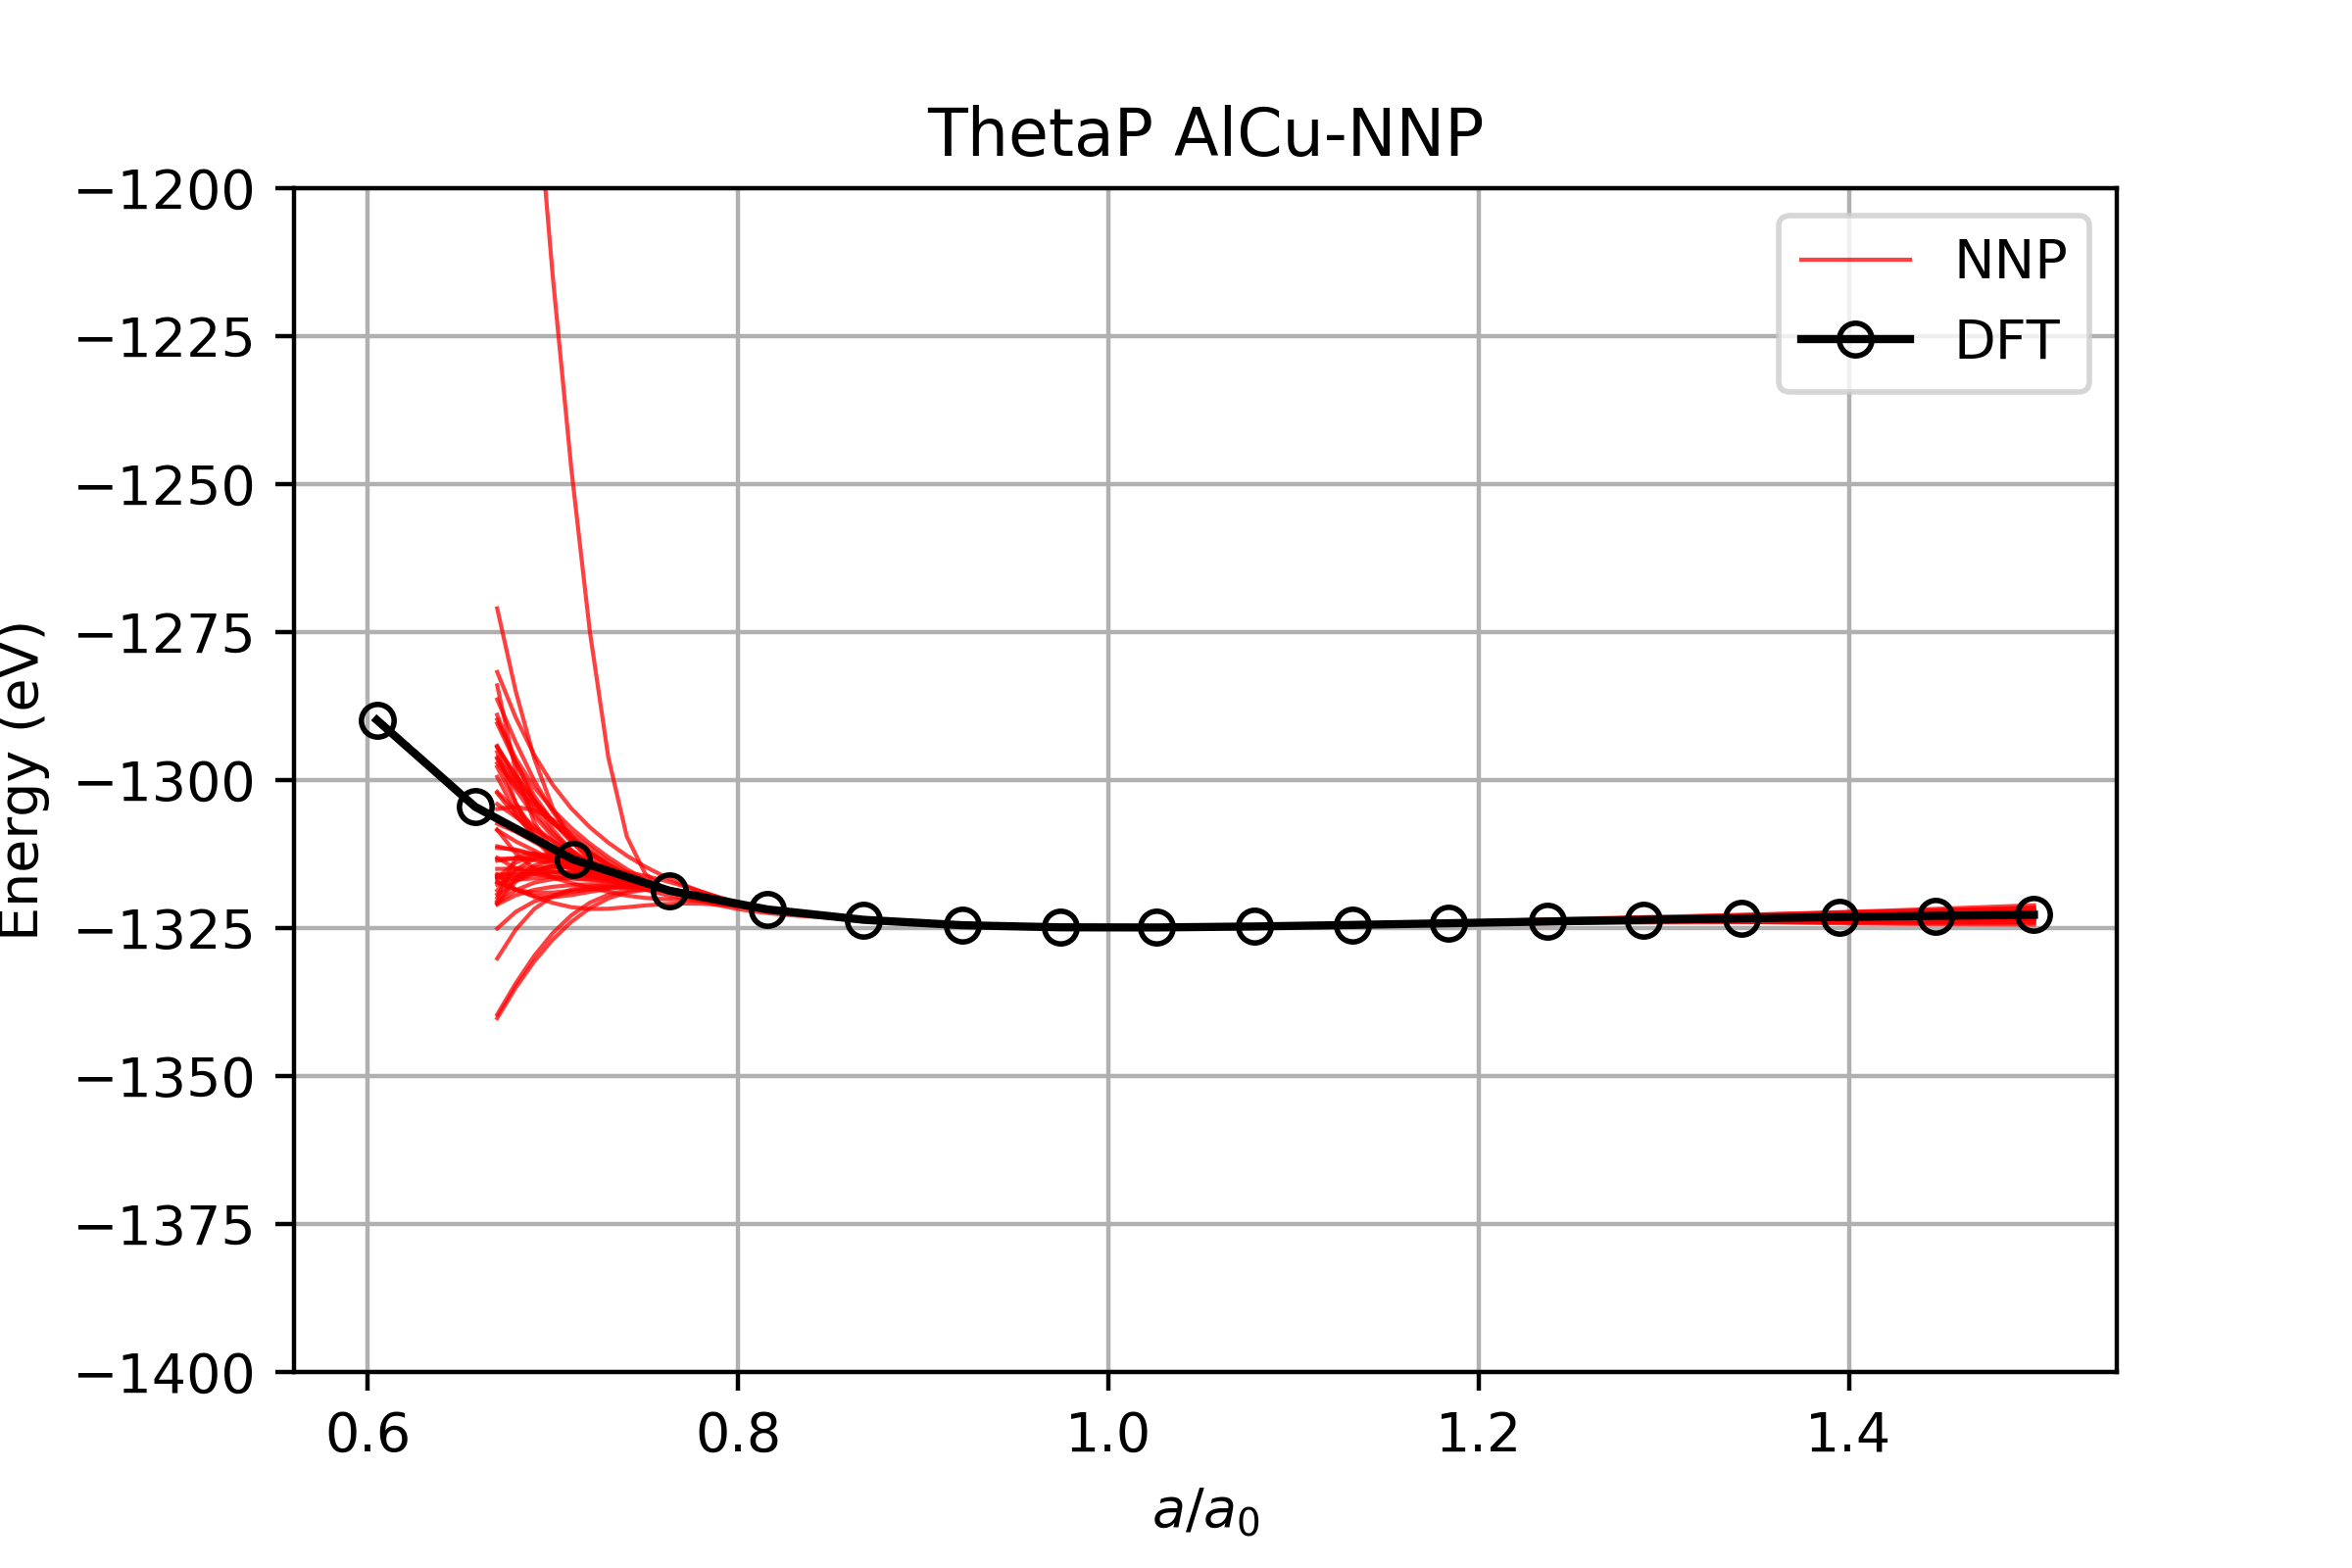
\includegraphics[width=0.7\textwidth,center]{figures/EOS_AlCu-NNP_ThetaP.png}%
\caption{$\theta'$ equation of state plot}%
\end{figure}

\begin{figure}[H]%
\centering%
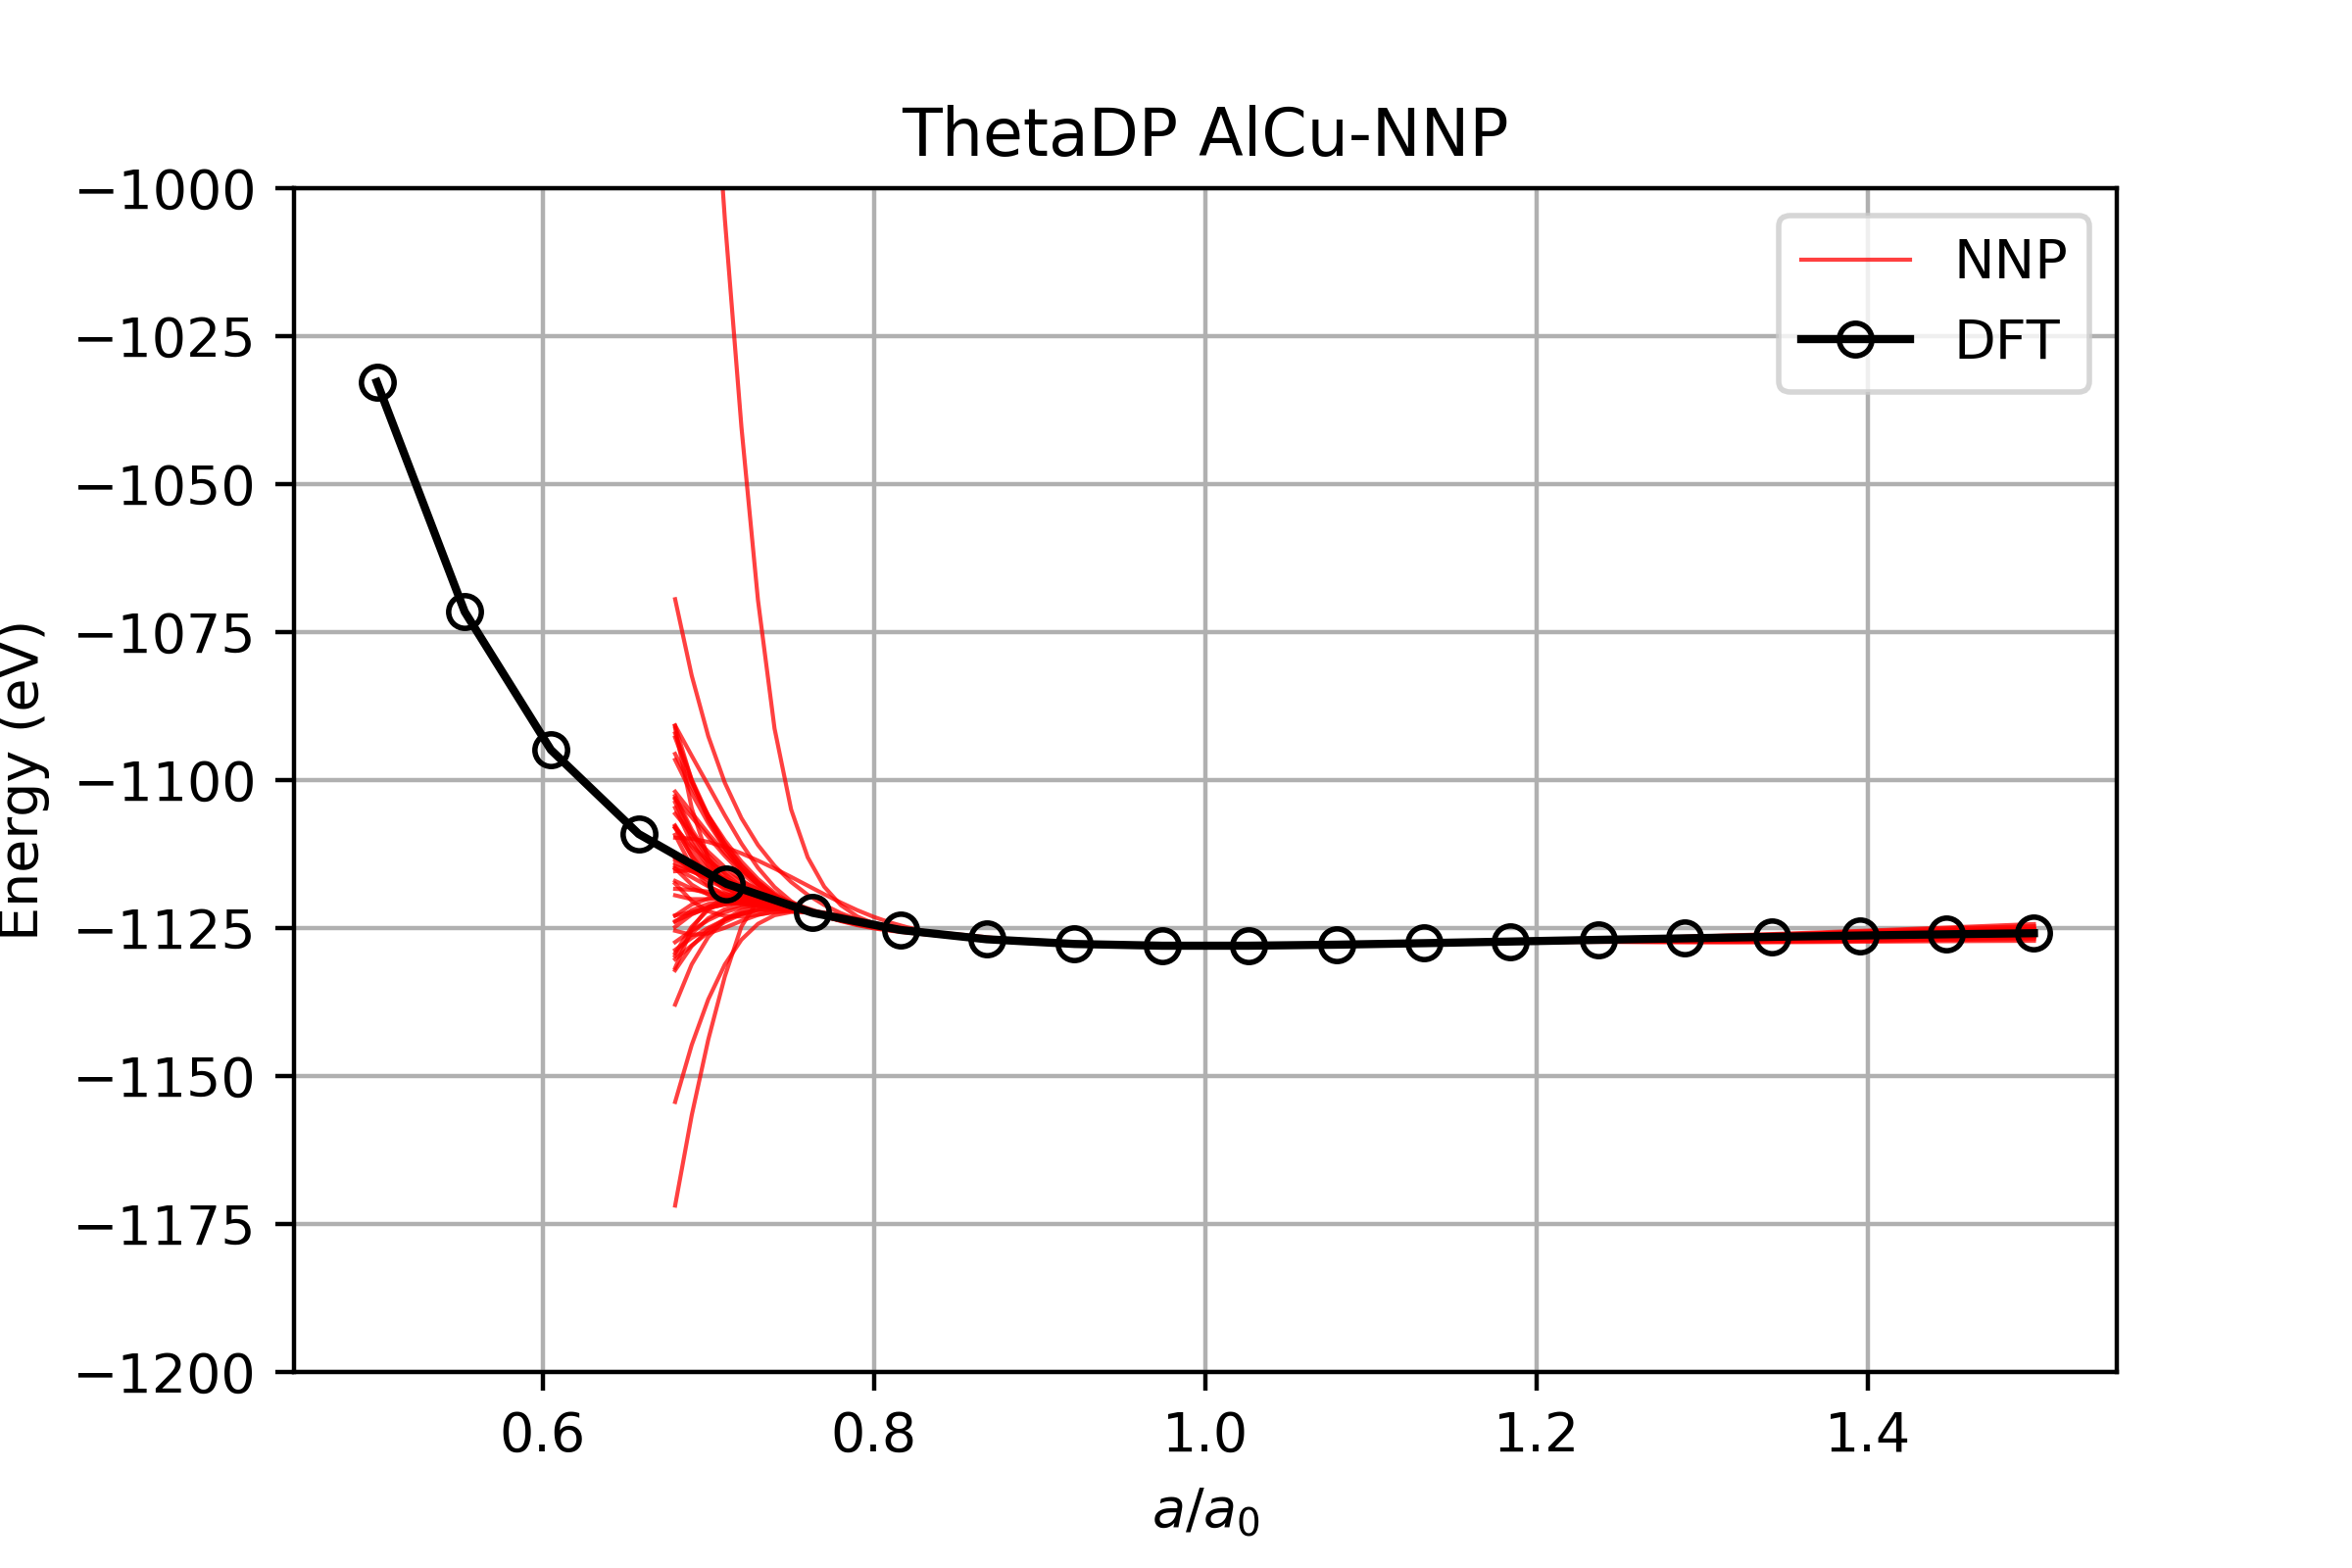
\includegraphics[width=0.7\textwidth,center]{figures/EOS_AlCu-NNP_ThetaDP.png}%
\caption{$\theta''$ equation of state plot}%
\end{figure}

\subsection{Additional Interface Formation Energy Plots} \label{sct:add_interface}
\begin{figure}[H]%
\centering%
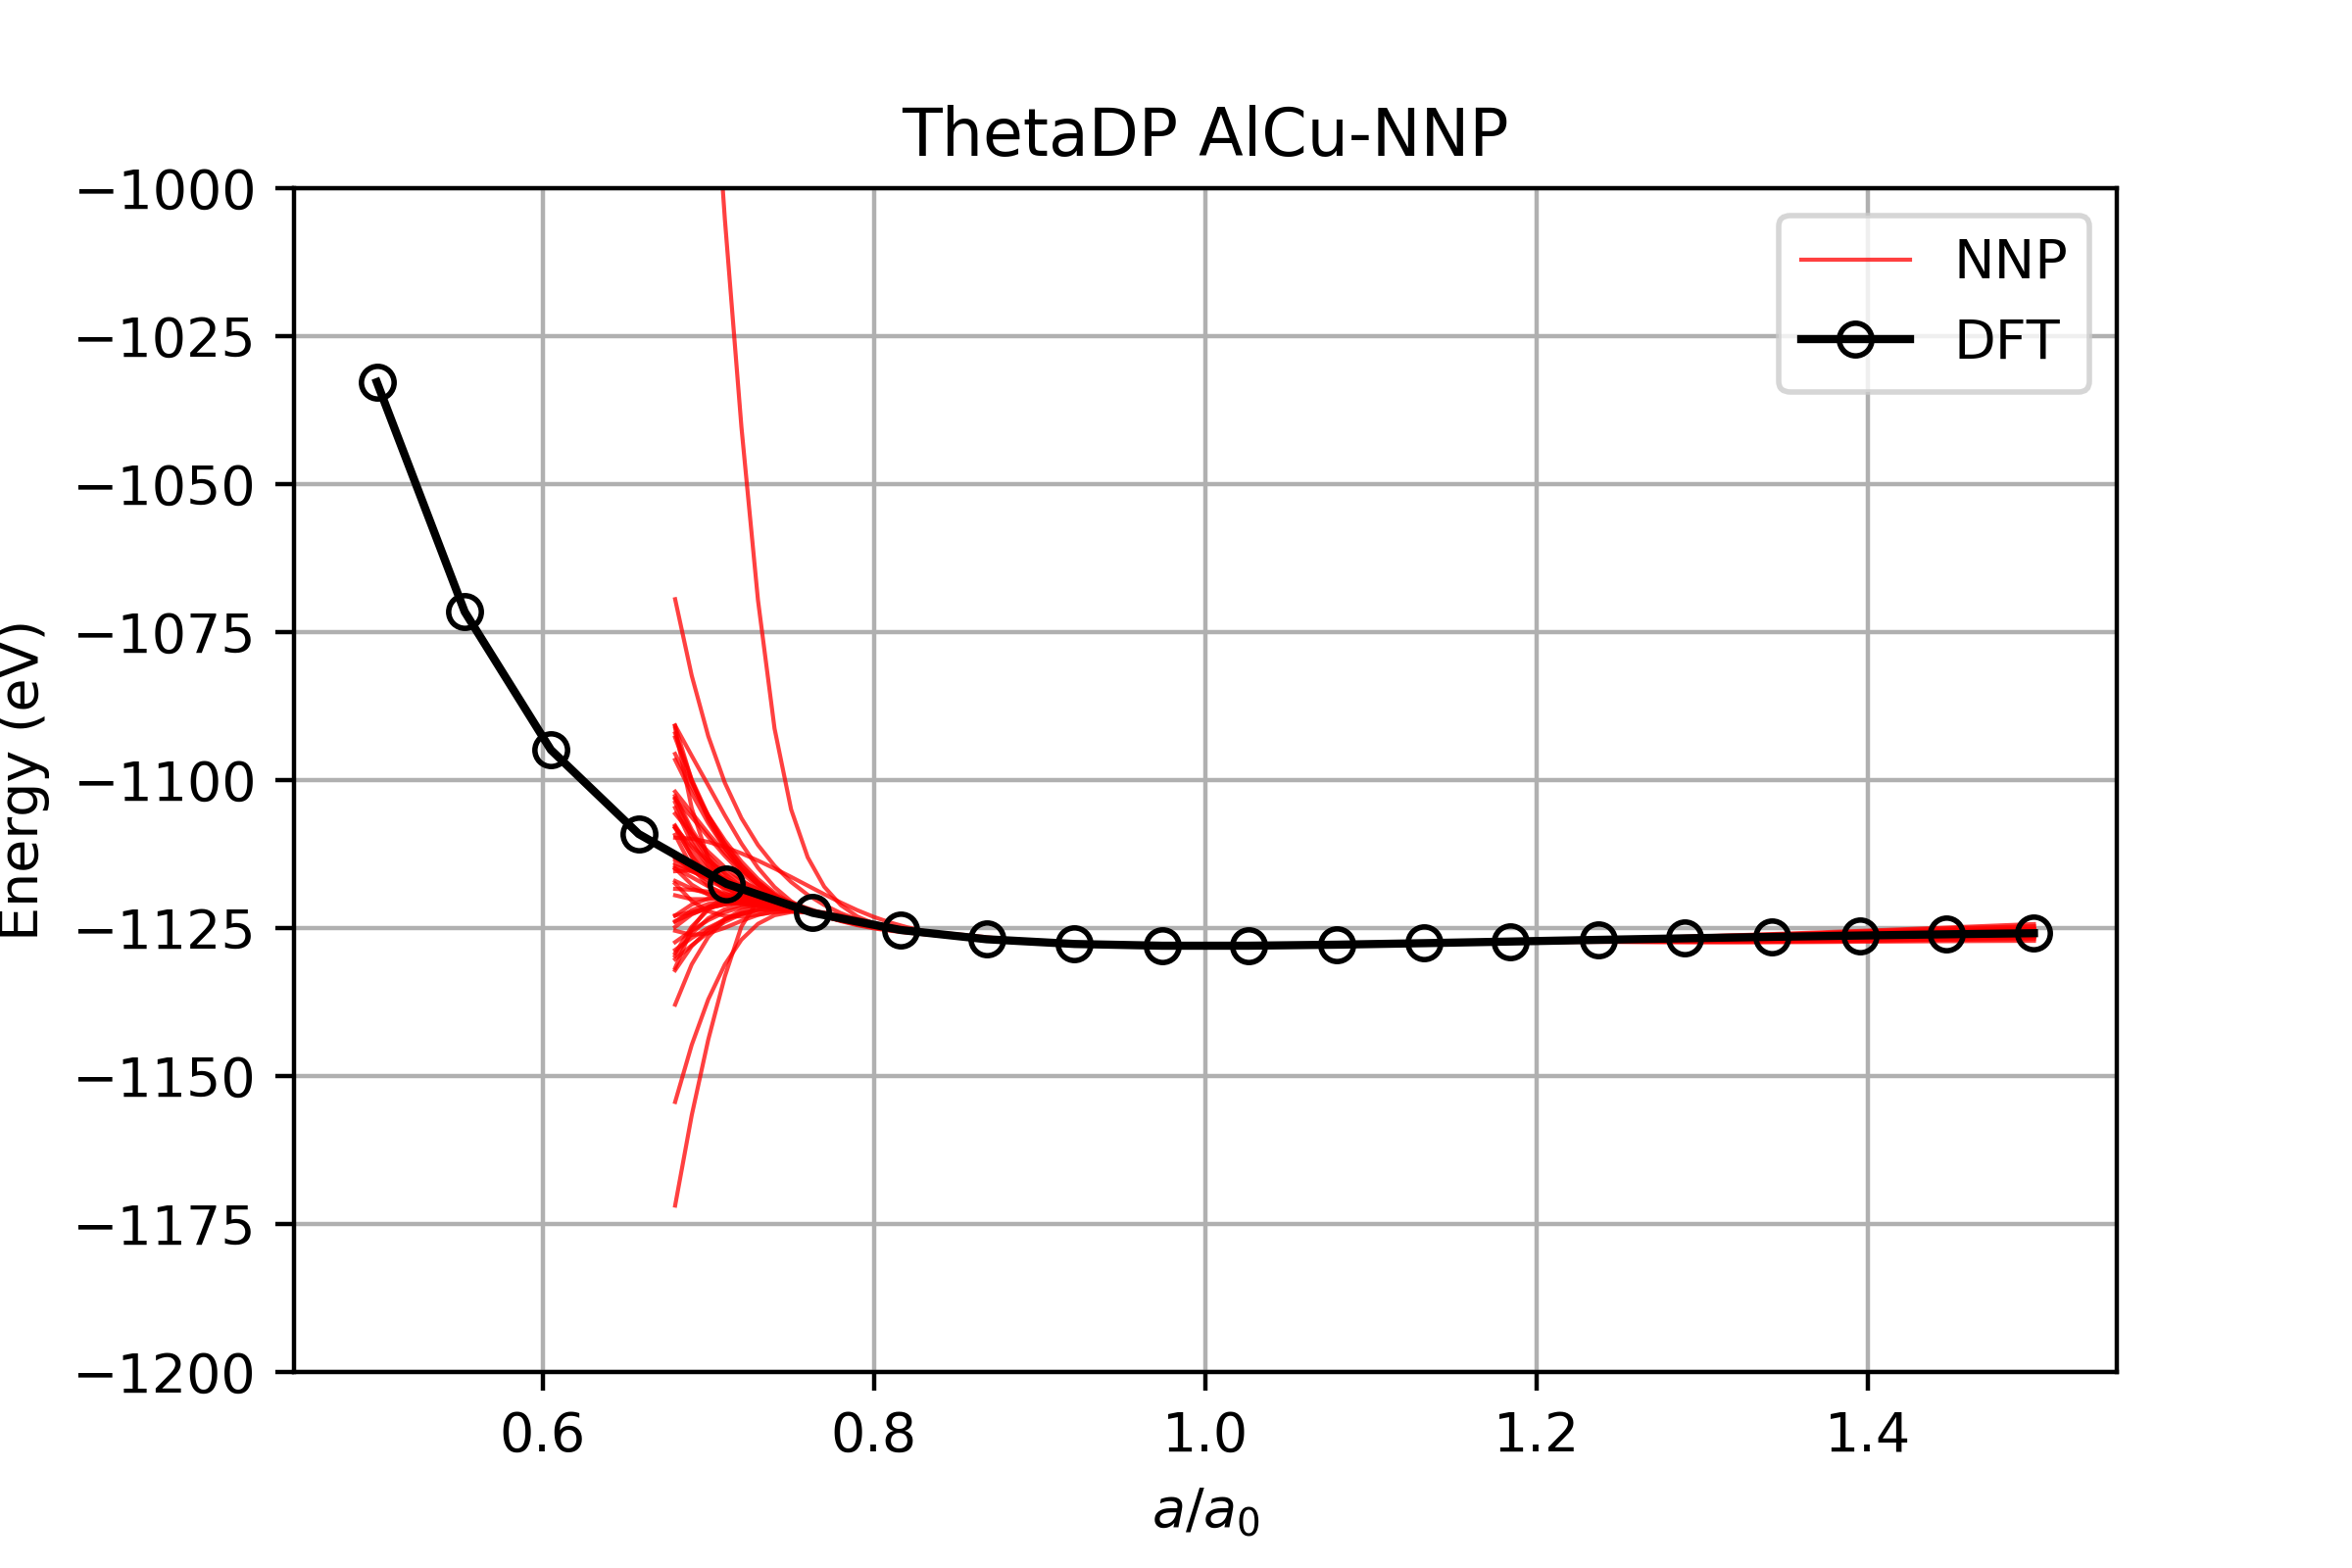
\includegraphics[width=0.7\textwidth,center]{figures/EOS_AlCu-NNP_ThetaDP.png}%
\caption{$\theta''$ equation of state plot}%
\end{figure}


\subsection{Additional Solute Plots} \label{sct:adn_solsol}
\subsection{}
\begin{figure}[H]%
\centering%
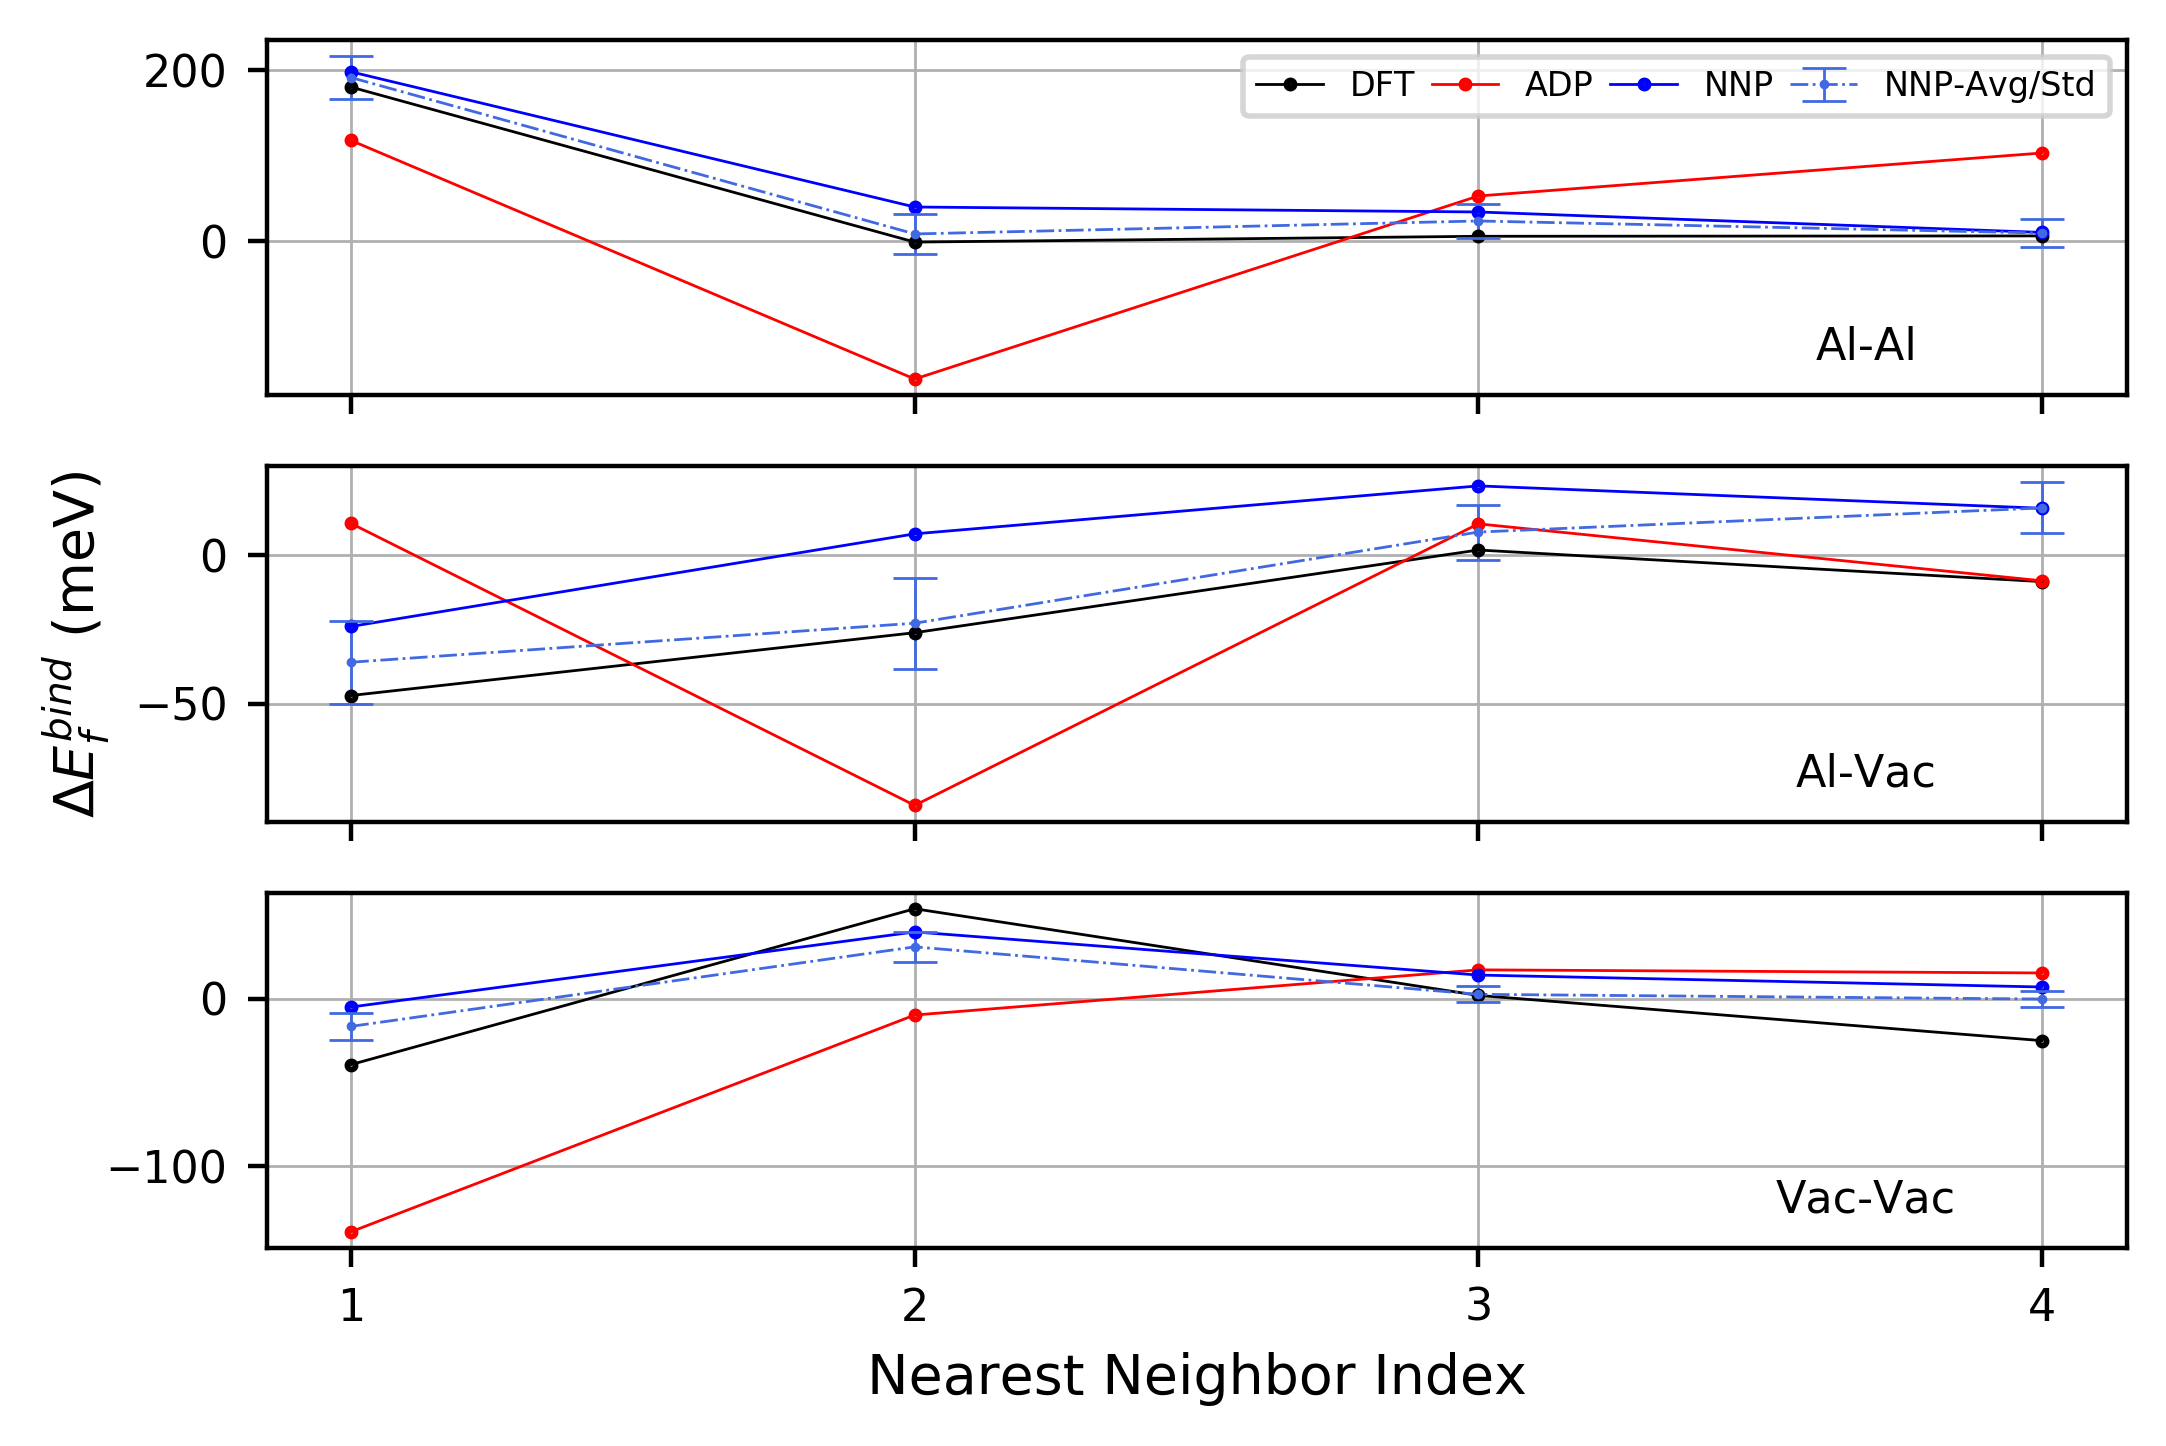
\includegraphics[width=1\textwidth,center]{./figures/solsol_in_cu.png}%
\caption{Neighbor index vs. binding energy $E_{bind}$ for Al-Al, Al-Vac and Vac-Vac in Cu matrix.}%
\label{fig:solsol_in_cu}
\end{figure}



\begin{tabular}{l|lll|lll}%
\hline%
Structure&\multicolumn{3}{c}{FCC Al}&\multicolumn{3}{c}{FCC Cu}\\%
Method&DFT&NNP&ADP&DFT&NNP&ADP\\%
\hline%
a ($\AA$)&4.04&4.047&4.05&3.625&3.627&3.615\\%
vol/atom ($\AA^3$)&16.48&16.58&16.61&11.9&11.93&11.81\\%
G (GPa)&30.7&33.0&29.6&59.4&62.6&55.3\\%
K (GPa)&78.2&77.2&78.5&143.9&146.3&138.9\\%
$C_{11}$ (GPa)&112.5&110.6&113.5&180.3&182.4&170.4\\%
$C_{21}$ (GPa)&61.0&60.5&61.1&125.7&128.2&123.2\\%
$C_{44}$ (GPa)&34.0&38.2&31.9&80.8&86.3&76.5\\%
\hline%
\end{tabular}%
\newline%
\newline%
\newline%
\newline%

\begin{tabular}{l|ccc|ccc|ccc}%
\hline%
Structure&\multicolumn{3}{c}{Al$_2$Cu  $\theta$}&\multicolumn{3}{c}{Al$_2$Cu $\theta'$}&\multicolumn{3}{c}{Al$_3$Cu $\theta''$}\\%
Method&DFT&NNP&ADP&DFT&NNP&ADP&DFT&NNP&ADP\\%
\hline%
a ($\AA$)&4.869&4.917&4.862&4.087&4.095&3.994&2.804&2.792&2.784\\%
b ($\AA$)&4.926&4.929&4.862&4.087&4.095&3.994&2.804&2.792&2.784\\%
c ($\AA$)&4.926&4.929&4.862&4.087&4.095&3.994&7.65&7.65&7.586\\%
$\alpha$&75.9&75.6&75.2&60.0&60.0&60.0&90.0&90.0&90.0\\%
$\beta$&60.4&60.1&75.2&60.0&60.0&60.0&90.0&90.0&90.0\\%
$\gamma$&60.4&60.1&60.6&60.0&60.0&60.0&90.0&90.0&90.0\\%
vol/atom ($\AA^3$)&14.88&14.95&14.41&16.09&16.18&15.02&15.04&14.9&14.69\\%
$\Delta$$H^{comp}$ (meV/atom)&{-}161.6&{-}162.9&{-}189.8&{-}184.0&{-}184.0&{-}202.6&{-}94.2&{-}94.8&{-}128.8\\%
G (GPa)&42.3&39.3&57.5&56.6&56.5&44.1&48.8&40.6&32.6\\%
K (GPa)&100.8&115.7&154.5&97.0&96.8&138.6&94.3&89.5&84.9\\%
$C_{11}$ (GPa)&170.4&167.8&199.5&158.7&160.4&192.4&160.5&148.6&115.4\\%
$C_{22}$ (GPa)&170.4&167.8&199.5&158.7&160.4&192.4&160.5&148.6&115.4\\%
$C_{33}$ (GPa)&174.8&180.4&278.2&158.7&160.4&192.4&181.8&154.1&142.0\\%
$C_{44}$ (GPa)&28.8&37.0&80.0&63.5&62.3&46.5&45.8&32.4&38.2\\%
$C_{55}$ (GPa)&28.8&37.0&80.0&63.5&62.3&46.5&45.8&32.4&38.2\\%
$C_{66}$ (GPa)&47.5&38.1&21.0&63.5&62.3&46.5&42.2&46.6&27.4\\%
$C_{21}$ (GPa)&73.7&104.2&99.3&66.2&64.9&111.6&70.9&61.6&48.0\\%
$C_{31}$ (GPa)&61.1&79.2&128.7&66.2&64.9&111.6&51.1&57.6&73.8\\%
$C_{32}$ (GPa)&61.1&79.2&128.7&66.2&64.9&111.6&51.1&57.6&73.8\\%
\hline%
\end{tabular}%



\end{document}
